\chapter{Desenvolvimento}
\label{cap:desenvolvimento}

Este capítulo descreve o desenvolvimento do  Sistema Inteligente Ágil de Processo Evolutivo - SIAPE, o qual segue o paradigma EPS. Para este desenvolvimento foi criado um método de desenvolvimento em que os princípios de EPS foram usados desde as fases mais primordiais do desenvolvimento. O método de desenvolvimento criado foi chamado de Método de Desenvolvimento de Sistemas Evolutivos - MeDSE. Duas seções foram utilizadas para realizar essa descrição: 

Na Seção 3.1 são descritas as três fases do método de desenvolvimento, a saber: Fase de Conceitos, Fase de Realizações e Fase de Finalizações. A seu turno, cada fase é composta por um número parcial de etapas, de um total de dez, que facilitam o desenvolvimento de cada fase.

A Seção 3.2 descreve a aplicação do método de desenvolvimento no protótipo SIAPE por meio das descrições dos desenvolvimentos de suas partes mecânica (descrição dos dispositivos definidos para a parte mecânica), eletrônica (a descrição dos circuitos elétricos), de software (descrição dos agentes mecatrônicos e seus \textit{skills})  e comunicação (descrição dos protocolos \textit{FIPA} utilizados na comunicação entre os agentes mecatrônicos do sistema) e suas  integrações.


%================================ VISÃO GERAL DO MEDSE =================================

\section{Visão do Método de Desenvolvimento de Sistemas Evolutivos (MeDSE)}

Para realizar o desenvolvimento do (SIAPE) identificou-se a necessidade da criação de um método que contemplasse a noção de agentes inteligentes e suas habilidades, que são denominados de \textit{skills} no paradigma \textit{EPS}, desde as primeiras fases do desenvolvimento. O método foi denominado de Método de Desenvolvimento de Processo Evolutivo (MeDSE). 

\begin{landscape}
 	\begin{figure}[h]
  		\centering
 		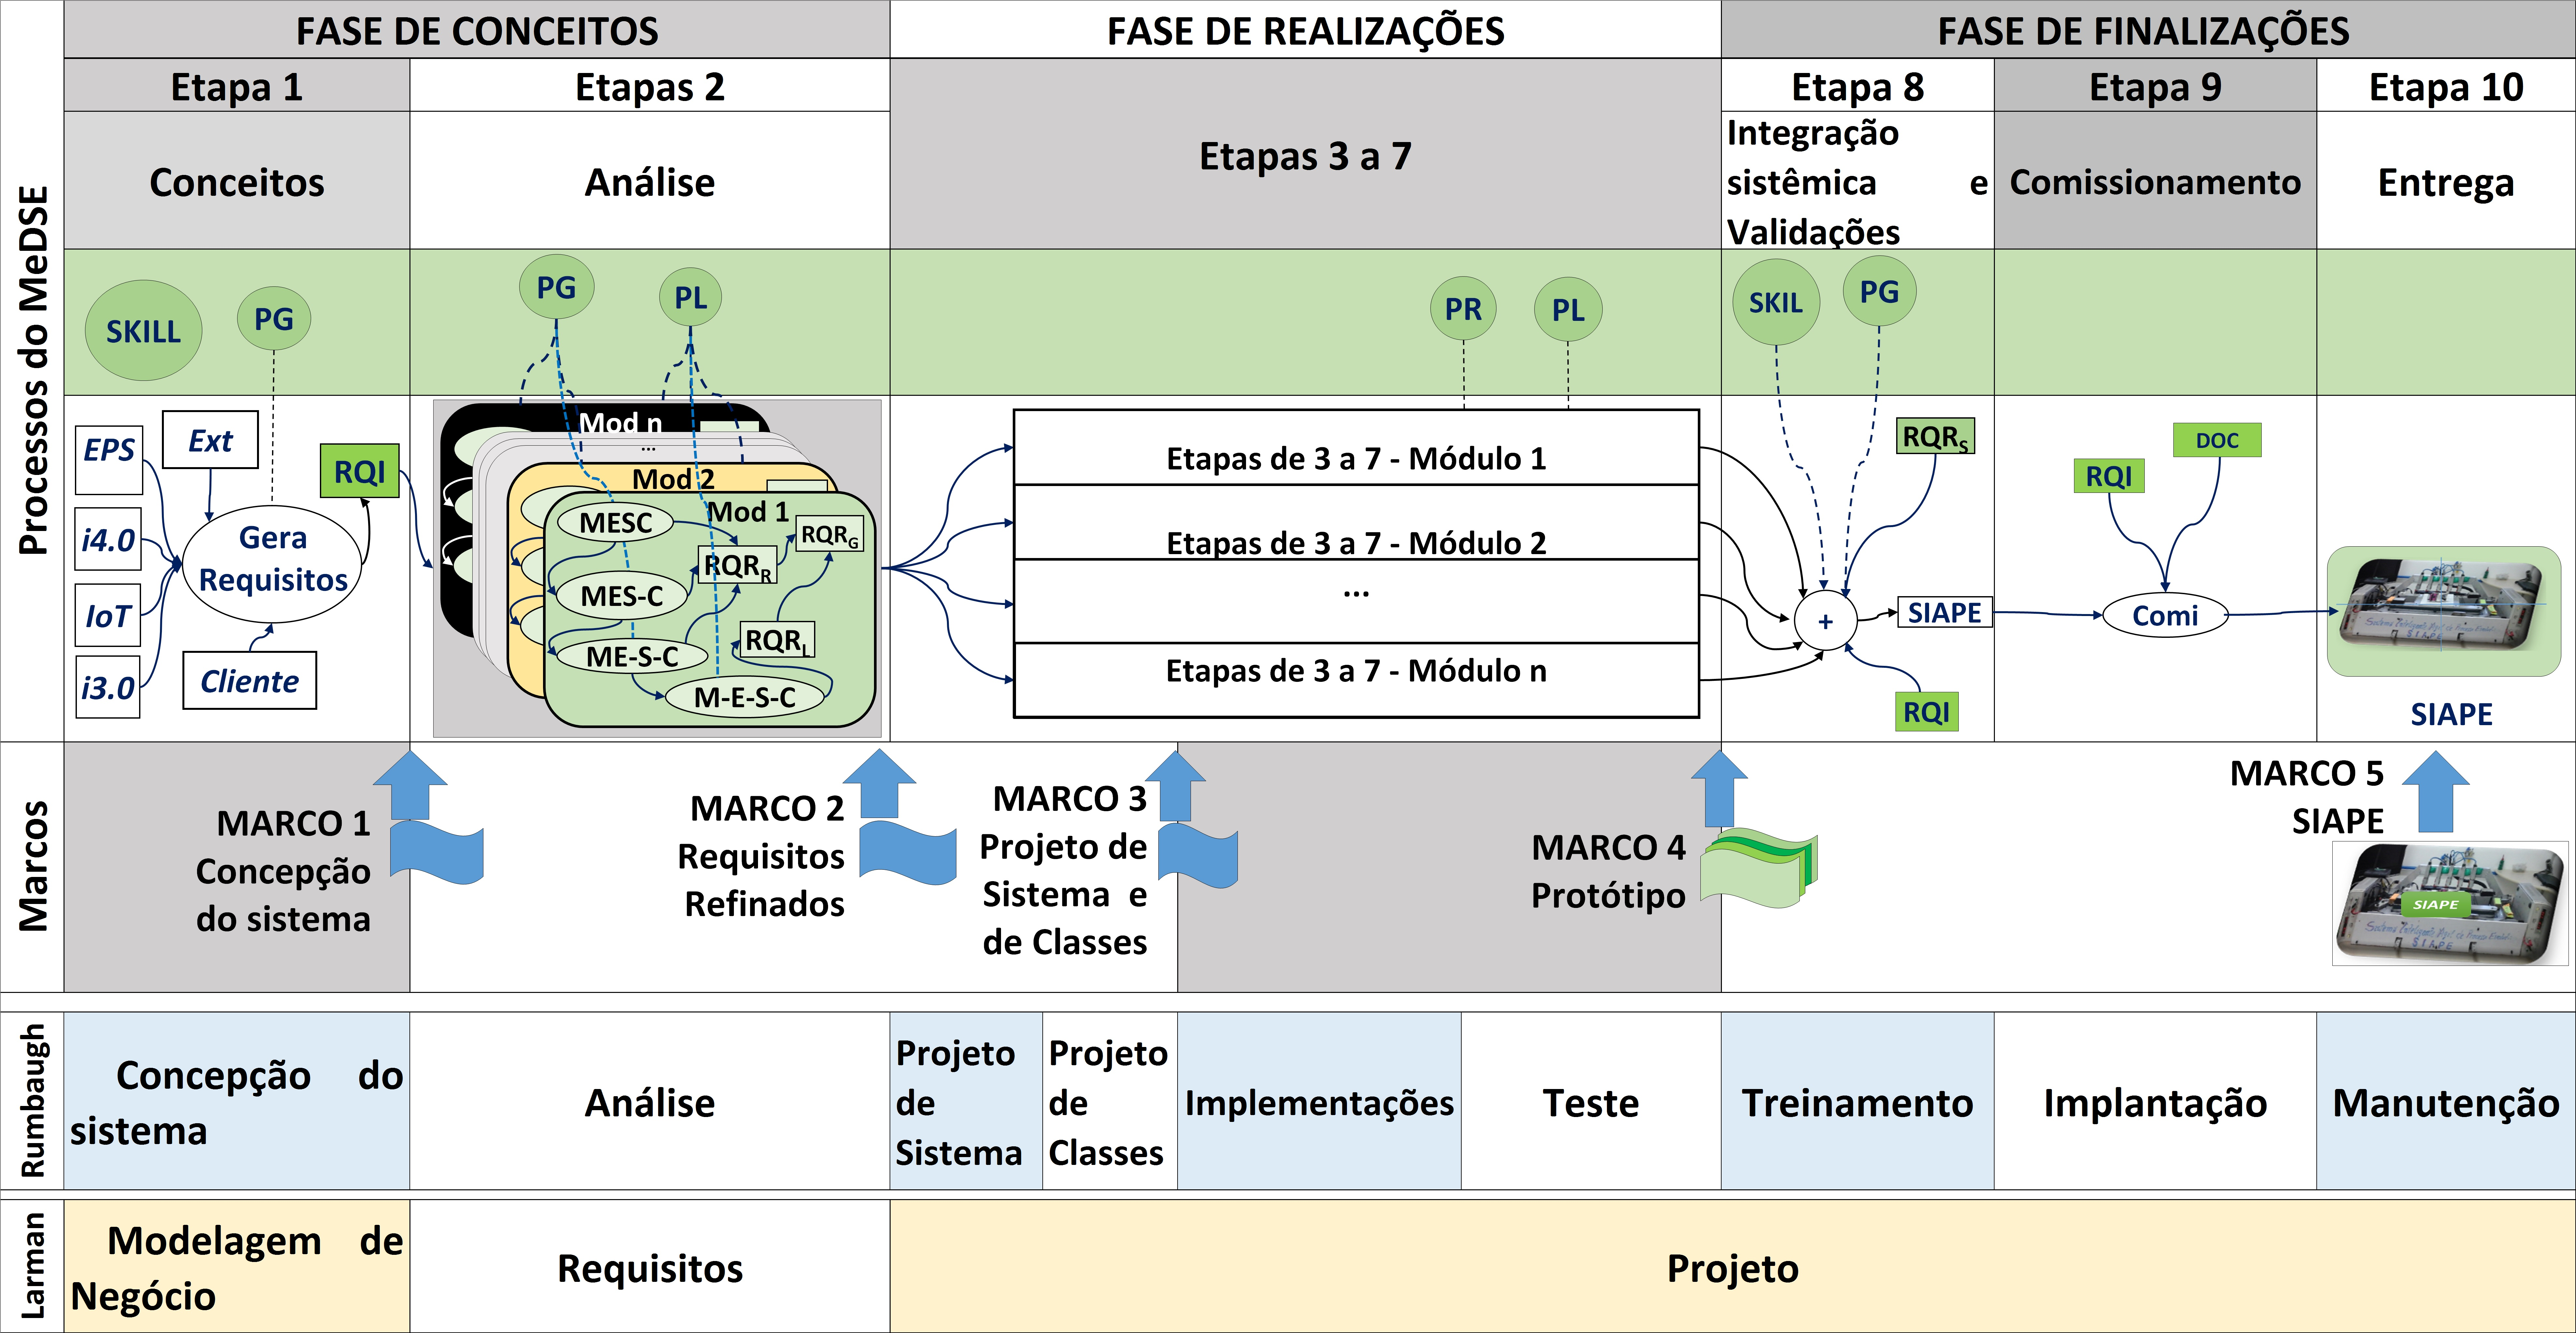
\includegraphics[width=20cm, height=14cm]{F25_SIAPE_VISAO8_1.jpg} 
 		\caption{Método de Desenvolvimento de Sistemas Evolutivos - MeDSE}
 		\label{F13_1}
 	\end{figure}
\end{landscape}
 
Depois de criado, o método foi comparado aos métodos utilizados por \citeonline{RUMBAUGH2006} e \citeonline{LARMAN2007}. A comparação com \citeauthor{RUMBAUGH2006} teve como principal objetivo a criação dos marcos do MeDSE. \textit{LARMAN 2007} foi utilizado para melhorar a acurácia na definição de requisitos e seus refinamentos. 
A Figura~\ref{F13_1} ilustra a visão geral do MeDSE na qual pode-se identificar as fases, as etapas, as atividades e os marcos a partir dos métodos comparados. Tais itens são explorado nas subseções seguintes.


\subsection{Definição de agente mecatrônico, problema global, problema regional e problema local}

Uma parte importante do MeDSE são os conceitos de Problema Global (PG), Problema Regional (PR) e Problema Local (PL).


A Figura \ref{F15}, mostra um esquema de como tais conceitos se relacionam. Nesta figura:
\begin{description}
	\item[M] - denota uma parte mecânica
	\item [E] - denota uma parte eletrônica
	\item  [S] - denota a parte de software
	\item  [C] - denota a parte de comunicação
	\item  [ME/MES/MESC] - Algum conjunto destas letras - corresponde a uma visão integrada daquelas partes. Ex.: ME é a integração entre a parte mecânica e a parte eletrônica.
	\item  [Cp] - é um componente composto, por exemplo, o SIAPE é uma composição de vários MESC.
	\item  [At] - é um componente visto de forma atômica. Ex.: a parte mecânica pode ser projetada de forma independente, segundo suas propriedades mecânicas, em relação às outras partes do sistema/subsistema/módulo.
	\item  [?] - denota um outro componente que pode ser qualquer um dos aqui discutidos.
	\item  [Propriedades] - uma ou mais característica, ou propriedade, ou atributos da entidade ou do sistema.
	\item  [Triângulo] - representa uma integração (composição) se vista de baixo para cima ou uma especialização (decomposição) vista de cima para baixo no diagrama.
\end{description}


\begin{figure}
	\centering
	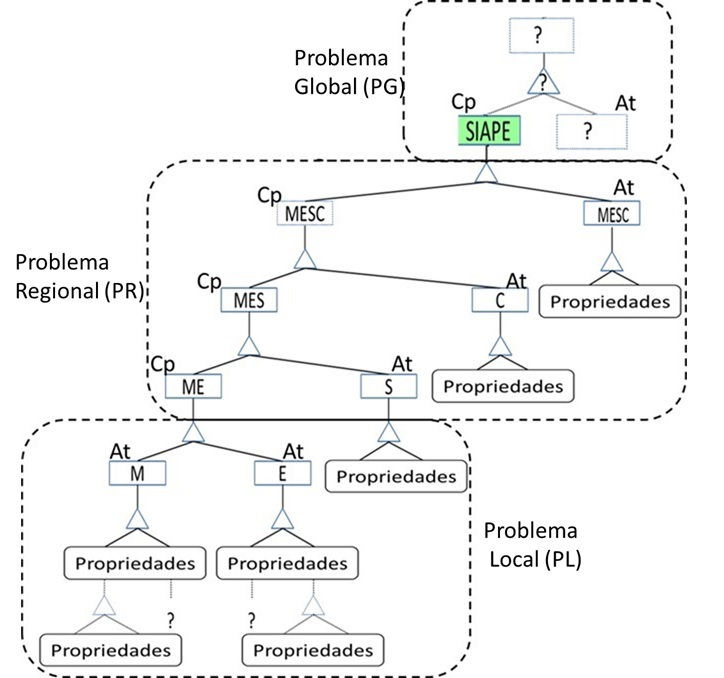
\includegraphics[width=10cm,height=8cm]{F15_PG_L.jpg} 
	\caption{MeDSE: Dividindo o problema global em regional e local}
	\label{F15}
\end{figure}

\begin{description}
	
\item[Definição de agente mecatrônico] - Neste trabalho, os agentes mecatrônicos são os módulos do sistema de manufatura e são identificados pela sigla MESC (Mecânica, Eletrônica, Software, Comunicação), indicando um sistema/subsistema/módulo completamente funcional.

Na Figura 3.2, um ou mais destes módulos serão integrados no sistema SIAPE.

\item[Definição de problema global (PG)] - Problema global é definido como a identificação do sistema como um todo e todas as partes a serem envolvidas. Essa identificação deve representar o consenso entre os especialistas da parte do cliente e a equipe de desenvolvimento. Por exemplo, um carro acoplado a um motor elétrico é integrado a um controlador, o qual contém um software que tem a capacidade de acelerar e parar o carro conforme ordens vindas pela rede. A Figura~\ref{F15} corresponde ao SIAPE.


\item[Definição de problema regional (PR)] - Problema regional é definido como uma visão do sistema na qual os relacionamentos entre as partes que o formam dependem funcionalmente uma das outras. Na Figura 3.2, por exemplo, ME e MES correspondem a dois problemas regionais. ME contém atributos/propriedades tanto mecânicos quanto eletrônicos, que formam então uma entidade de nível mais alto, integrada. MES, por outro lado, contém atributos/propriedades mecânicas, eletrônicas e de software. Formam uma entidade de nível ainda mais alto, quase um módulo completo.
Já MESC é outro problema regional e que denota um módulo completo, um agente mecatrônico.

\item[Definição de problema local (PL)] - Problema Local é definido como a visão em que as entidades que formam o sistema são atômicas, isto é, podem ser analisadas e desenvolvidas sem interferência de outras entidades. Na Figura~\ref{F15}, as entidades M e E, que correspondem aos conjuntos Mecânicos e Eletrônicos, podem ser analisadas individualmente com seus atributos e propriedades eletrônicas e mecânicas separadamente. Por exemplo: no conjunto mecânico, uma especificação possível pode aparecer como: um carro deve movimentar-se sobre um trilho; tanto a largura do carro e a bitola do trilho são especificadas sem nenhuma influência da parte eletrônica e podem ser analisados pela equipe mecânica sem restrições. O motor que faz o carro funcionar, pode igualmente ser especificado em termos de torque e velocidade mecânicos, mas a equipe eletrônica pode fazer análise de seu funcionamento independentemente da mecânica.\par 

Ainda analisando a Figura \ref{F15} pode-se perceber que as entidades M e E não conseguem mais ser decompostas em outras entidades, pois encontram-se em suas formas atômicas. Quando uma entidade atinge a sua forma atômica, o projetista chegou ao nível ideal para realizar a modelagem da entidade, pois em sua forma atômica, a entidade não sofre interferências de outra entidade externa. A tentativa de decompor a entidade levará ao nível das propriedades da entidade decomposta, ou seja, levará à desestruturação da mesma, inviabilizando o processo de modelagem. \par  

\end{description}


\subsection{A Fase de Conceitos}
  
A Fase de Conceitos corresponde  à realização conceitual, isto é, a concepção do sistema e a definições dos requisitos conforme \citeonline{RUMBAUGH2006} e \citeonline{LARMAN2007}. O objetivo dessa fase é estabelecer uma visão comum entre as equipes de desenvolvimento e os representantes do cliente e o escopo básico do projeto. Seus procedimentos partem da consideração de que existe um problema global que deve ser subdividido em problemas menores para serem tratados atomicamente até se tornarem requisitos que são modelados e simulados para que possam garantir a definição das especificações das partes do sistema.
 
Essa fase é composta por duas etapas ilustrada na Figura \ref{F27_1} e são descritas nas próximas subseções.
 
\begin{figure}[h]
 	\centering
 	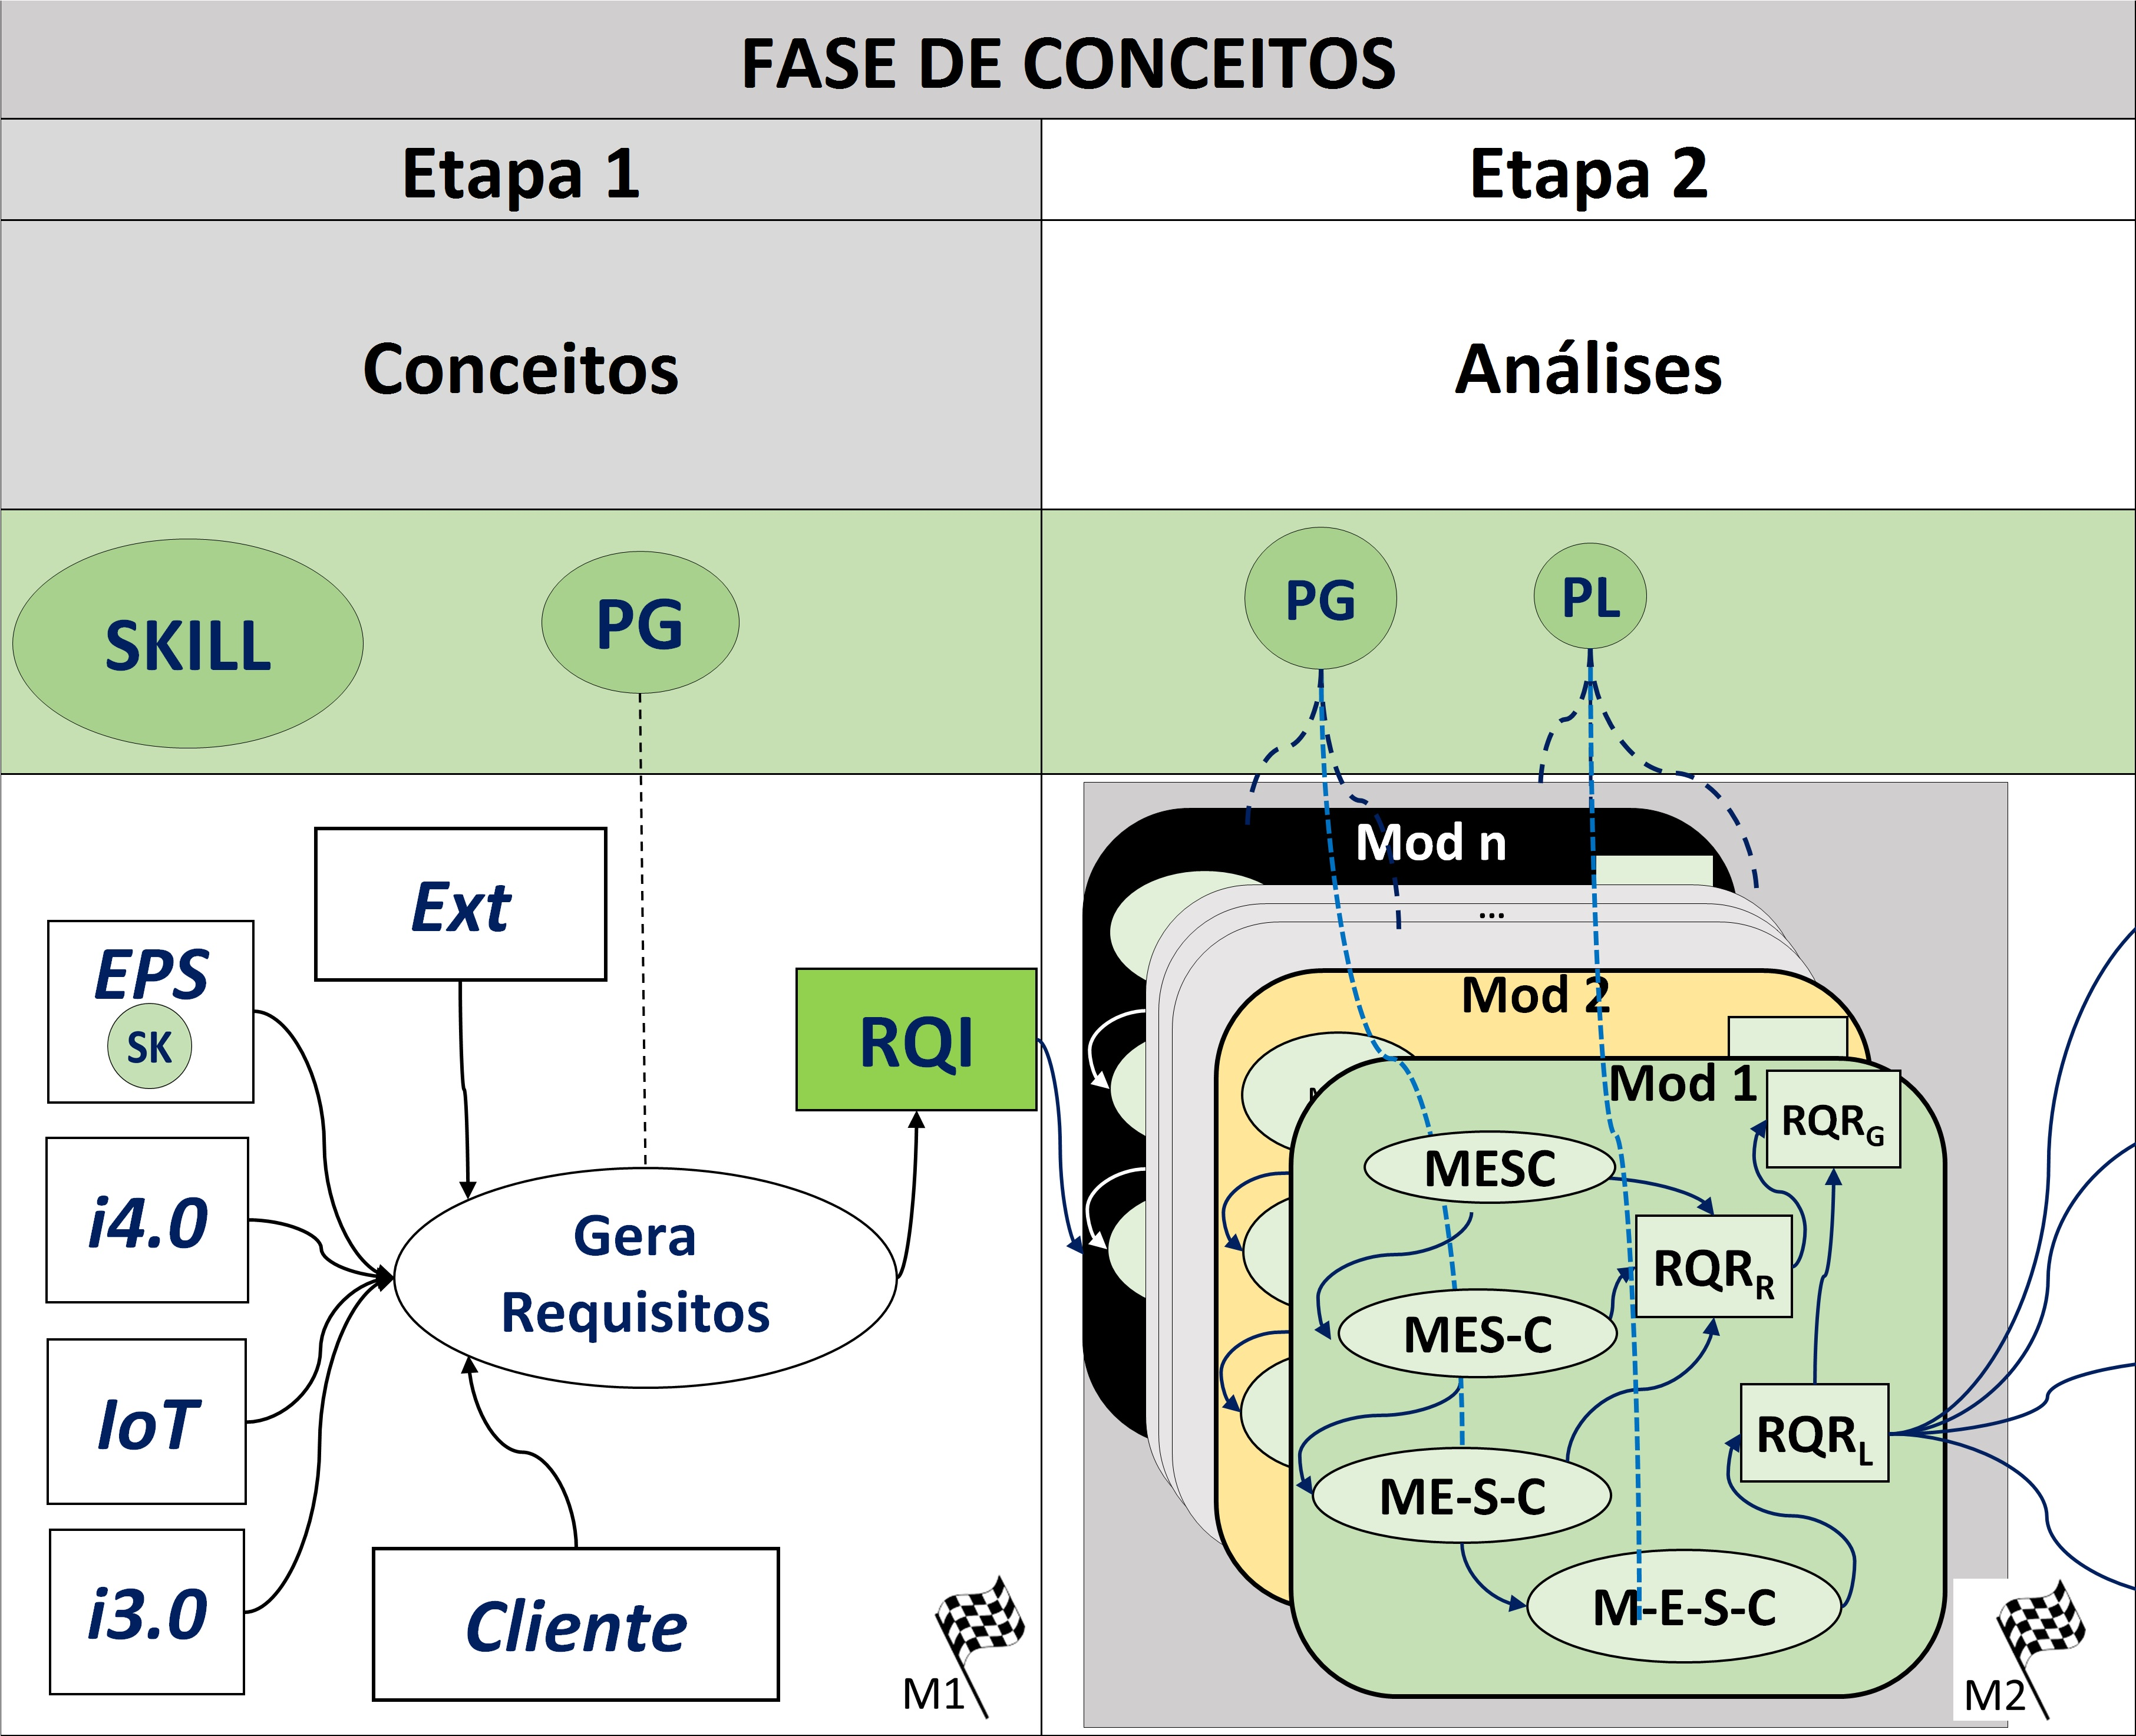
\includegraphics[width=10cm, height=5cm]{F27__SIAPE_FASE1.jpg} 
 	\caption{MeDSE: Fase de Conceitos}
 	\label{F27_1}
\end{figure}
 
\begin{description}
 	 \item[Etapa 1 - Conceitos] - A Etapa 1 tem como entrada as informações relativas ao sistema e as necessidades do cliente e sua saída é um documento de definição da concepção do sistema que contém os Requisitos Iniciais (RQI). Além da concepção do sistema, que deve ser aprovado por ambas as partes, desenvolvedores e cliente, o documento de expressar o que é o sistema, e quais os problemas a serem tratados pela equipe de desenvolvimento. A realização desta etapa evidencia a entrega do primeiro marco do sistema.
 	 
 	 \item[Etapa 2 - Análises] -  Na Etapa 2 os RQI são analisados como Problemas Globais (PG) e refinados em problemas regionais (PR) até que se consiga um nível atômico denominado de problema local (PL). Esses problemas são analisados considerando os conceitos de skills, que são as habilidades de agentes mecatrônicos, de problema global (PG), problema regional (PR) e problema local (PL). Com a realização desta etapa o segundo marco é entregue.  
 	 
 \end{description}
 

\subsection{A Fase de Realizações}
 
A Fase de Realizações corresponde aos processos práticos do desenvolvimento, isto é, à realização das etapas de Projeto de Sistema, Projeto de Classes, Implementações e Testes, conforme \citeonline{RUMBAUGH2006} e à Etapa de Projeto de \citeonline{LARMAN2007}. Nesta fase os requisitos refinados são modelados, simulados, transformados em projetos a partir das especificações técnicas, integrados e validados modularmente. Ao final dessa fase é entregue um protótipo funcional que evidencia o quarto marco.
 
Esta fase é formada pelas Etapas 3 a 7, mostradas de forma geral para n módulos na Figura 3.1, e que são mostradas em detalhes na Figura \ref{F13_2}. As seções seguintes descrevem cada uma destas etapas.
 	
\begin{figure}[h]
	\centering
	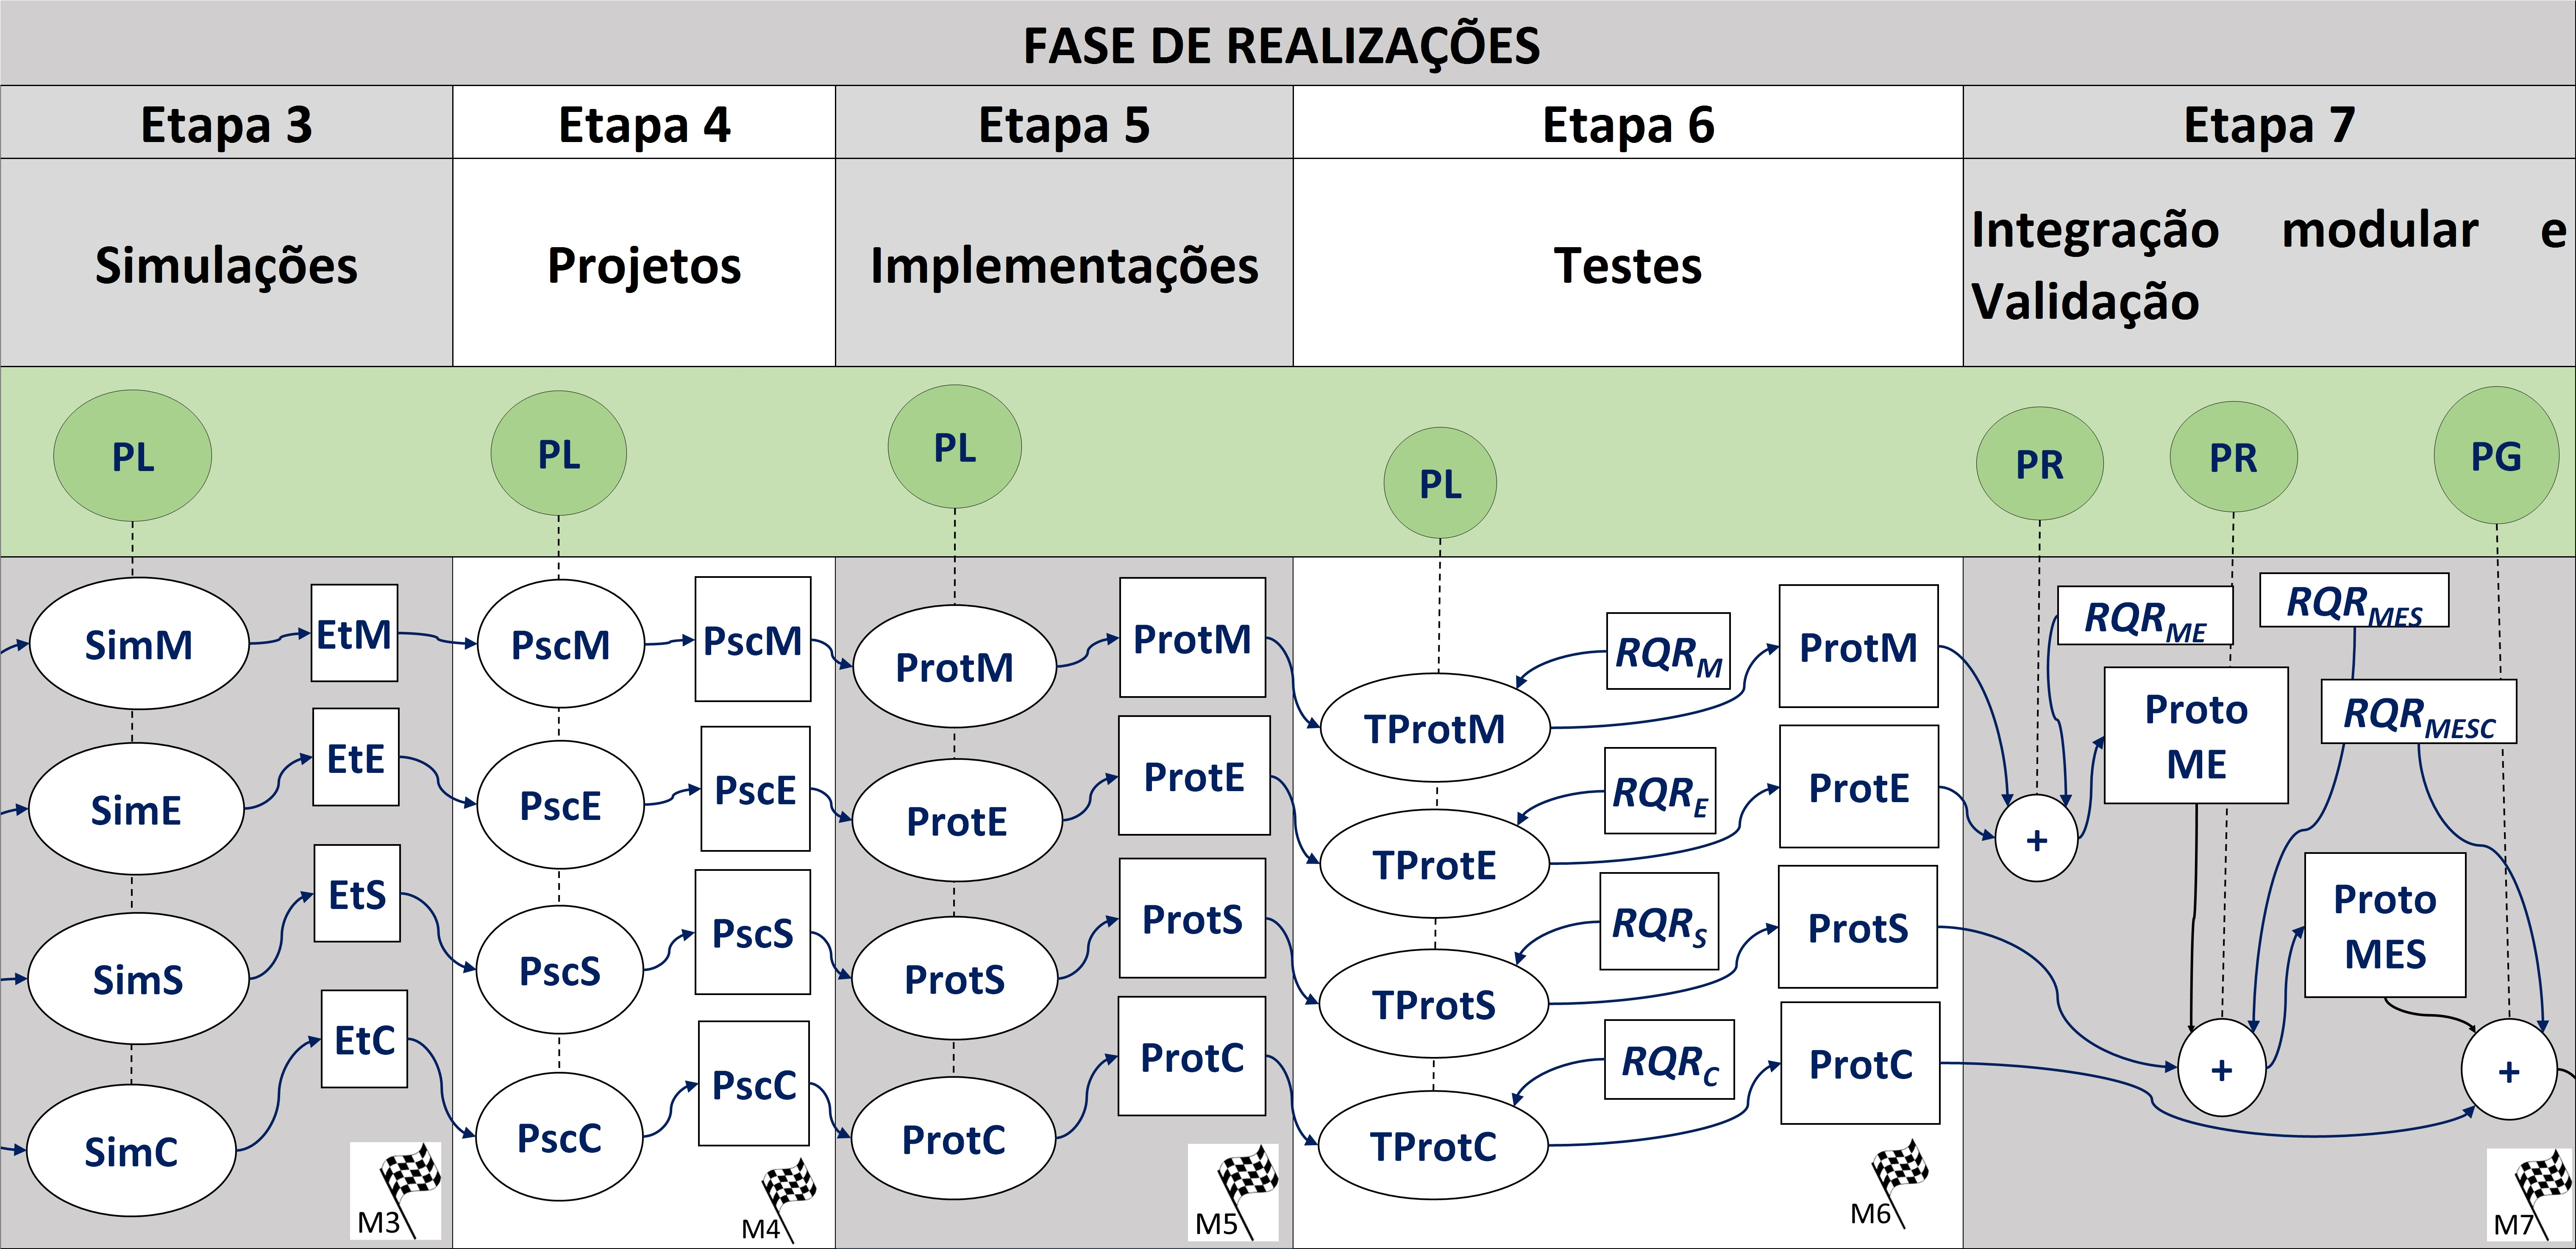
\includegraphics[width=16cm, height=7cm]{F25_SIAPE_VISAO8_1REAL.jpg} 
	\caption{MeDSE - Fase de Realizações}
	\label{F13_2}
\end{figure}
 	
\begin{description}
 	
  \item[Etapa 3 - Simulações] - Na Etapa 3 os requisitos refinados do sistema em forma de problema global (RQRs), na forma regional  (RQRr) e local (RQRl) são modelados e simulados (SimM, SimE, SimS e SimC) até que estes possam ser garantidos para serem confirmados como Especificações Técnicas (Et) de cada problema local, a saber: Especificação Técnica Mecânica (EtM), Especificação Técnica Elétrica (EtE), Especificação Técnica de Software (EtS) e Especificação Técnica de Comunicação (EtC). 
  
  
  \item[Etapa 4 - Projetos] - Na Etapa 4 as especificações técnicas são realinhadas na forma de projetos parciais para formarem o Projeto de Sistema e de Classes de cada problema local (PscM, PscE, PscS e PscC). Nesta etapa cada problema local tem suas especificações refinadas e incluídas no documento de projeto do sistema e entregue como evidência do quarto marco.  
  
  
  \item[Etapa 5 - Implementações] -  Nesta etapa os projetos de cada problema local são implementados, marcando as realizações iniciais dos protótipos locais: Os protótipos da parte mecânica (ProtM), da parte eletrônica (ProtE), da parte de software (ProtS) e da parte de comunicação (ProtC) tornam-se plantas reais dos projetos locais. 
  
  
  \item[Etapa 6 - Testes] - Nesta fase os protótipos construídos são submetidos aos processos de teste (TProtM, TProtE, TProtS e TProtC) contra os requisitos refinados de cada problema local (RQRm, RQRe, RQRs e RQRc). Após a aprovação são levados à condição de protótipos testados e aprovados para o processo de integração.
  
  \item[Etapa 7 - Integração e validação modular] -  Na Etapa 7 os protótipos testados são submetidos ao processo de integração e validação modular:
  
  \begin{enumerate}
  	
  	\item O protótipo mecânico (ProtM) é integrado ao protótipo eletrônico (ProtE) o qual denomina-se protótipo ME (ProtoME);
  	\item O Protótipo ME é então submetido ao processo de validação modular contra os requisitos refinados da entidade ME (RQRme) que representa a realização da solução para a problema regional (ME);
  	\item O ProtoME é integrado ao protótipo da parte de software (ProtS) e a essa integração denomina-se por MES (ProtoMES);
  	\item O protótipo MES é então submetido ao processo de validação modular contra os requisitos refinados da entidade MES (RQRmes) que representa a realização da solução para o problema regional MES;
  	\item O ProtoMES é então integrado ao protótipo da parte de comunicação (ProtC) e com essa integração chega-se à realização da solução do problema global MESC;
  	
  	O protótipo MESC é, então,  enviado à próxima etapa para ser submetidos aos testes de integração e validação sistêmica. 
  	
  \end{enumerate}
  
  Ao final das cinco etapas da fase de realizações, o módulo mecatrônico é concluído.
  
  Tais etapas devem ser realizadas para cada um dos módulos do sistema, que compõem a solução ao PG.
  
  Em todas as etapas do MeDSE existem realimentações de registros que informam se as atividades realizadas estão sendo cumpridas e se as metas de cada etapa foram alcançadas.  Caso não se atinja o desempenho esperado, a etapa é revista objetivando o alcance das metas e a entrega dos marcos do sistema. A Figura \ref{F29} ilustra as realimentações do sistema.
  
  \begin{figure}[h!]
  	\centering
  	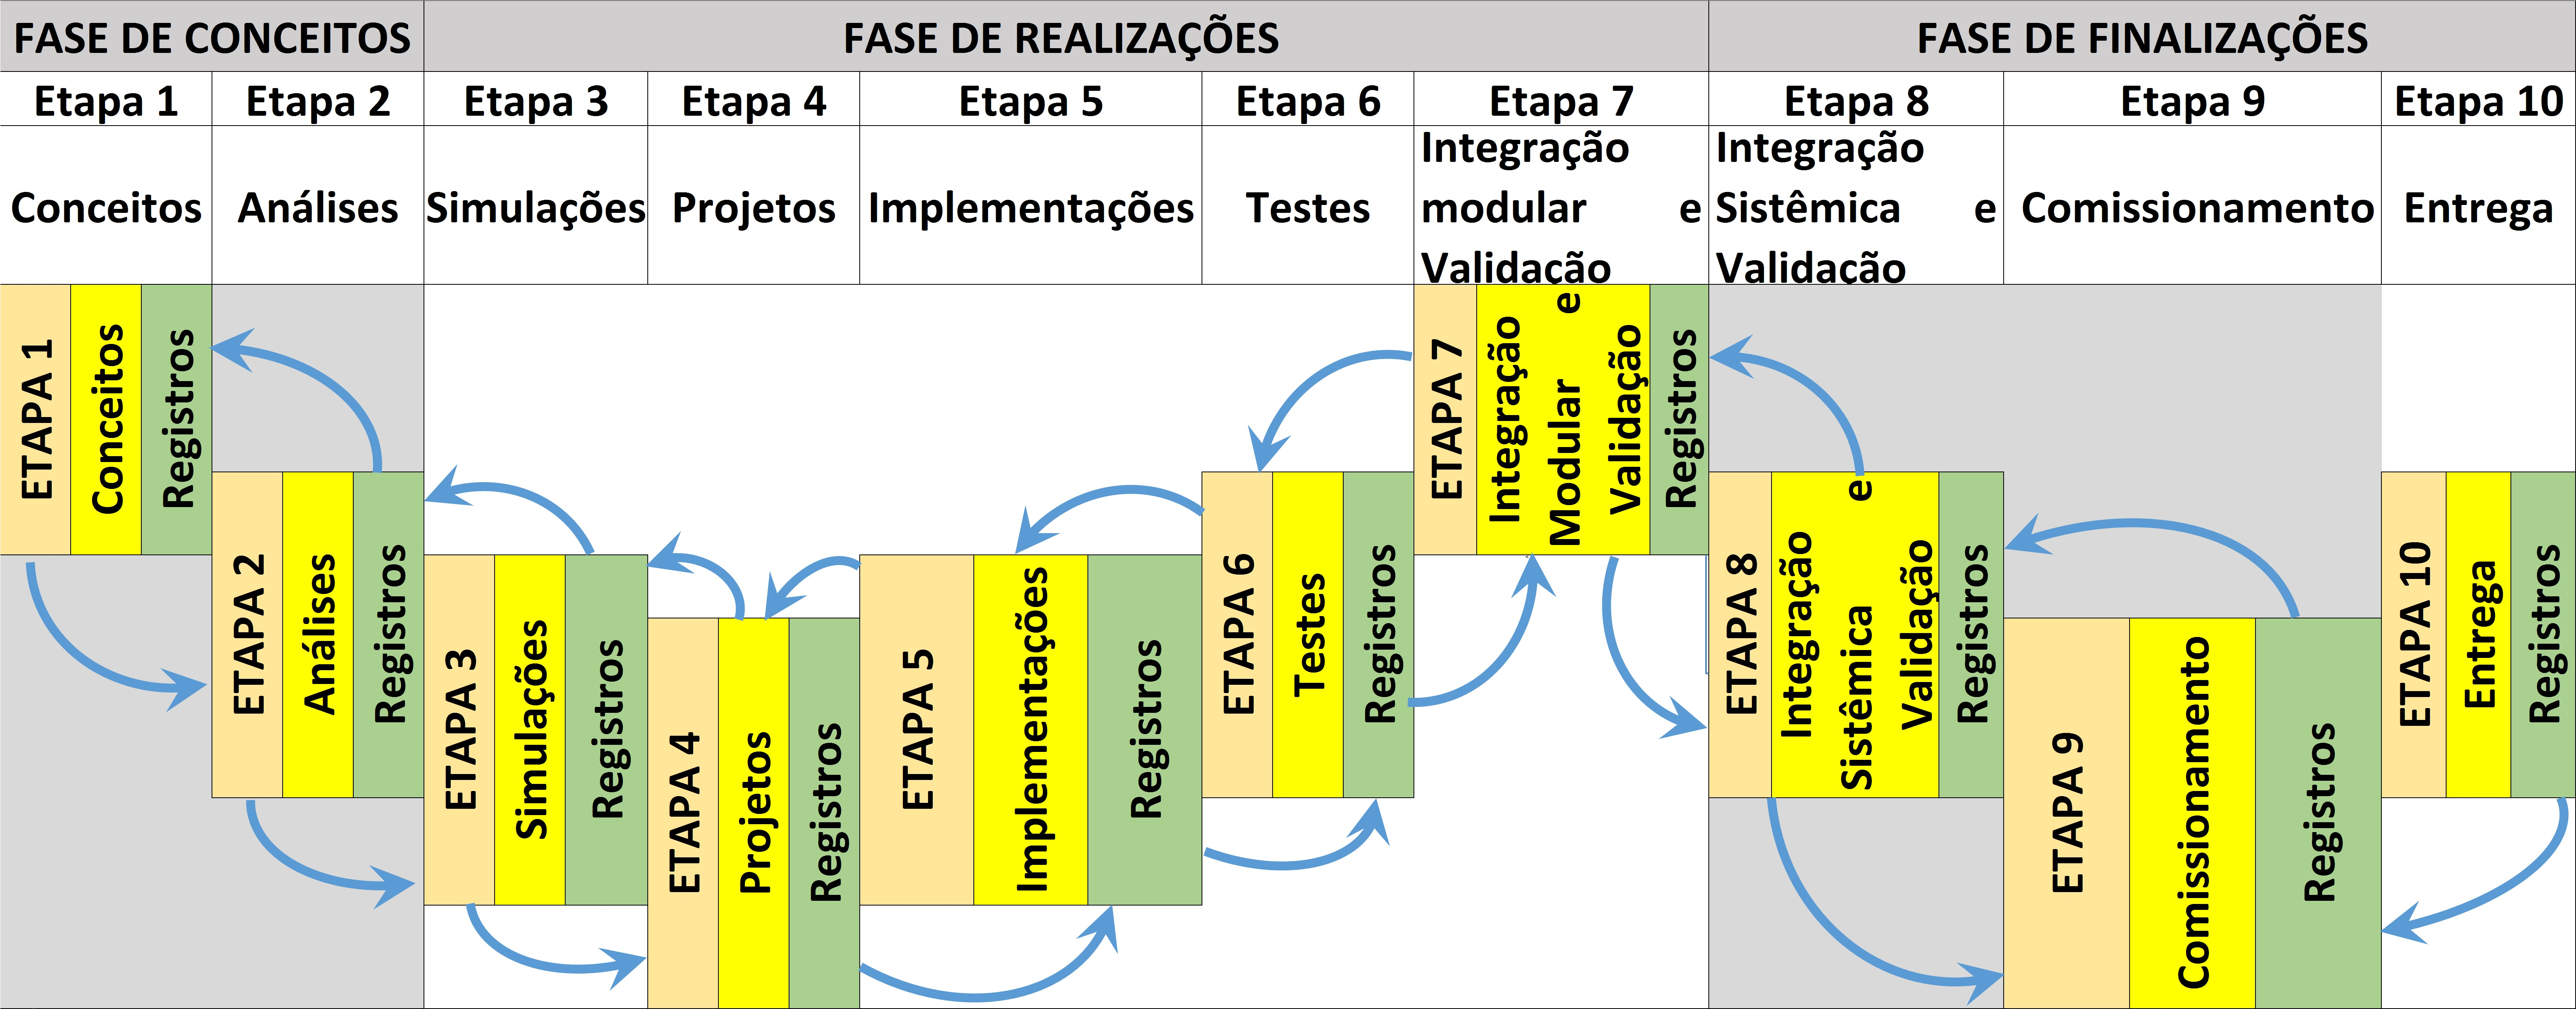
\includegraphics[width=16cm, height=7cm]{F27_SIAPE_REALIMENTACOES1.jpg} 
  	\caption{MeDSE: Realimentações do método}
  	\label{F29}
  \end{figure}
   
\end{description}
 
 
\subsection{A Fase de Finalizações}
 
A Fase de Finalizações tem o principal objetivos de verificar e validar a integração sistêmica do sistema desenvolvido para posterior comissionamento e entrega. A verificação neste trabalho é entendida como a atividade que analisa se os requisitos funcionais e não-funcionais foram atendidos, enquanto a validação analisa se as necessidades do cliente foram atendidas. A verificação e a validação aplicadas nesta fase se justifica devido ao fato do sistema estar totalmente integrado, isto é, antes que o sistema seja entregue ao cliente, a equipe de desenvolvimento deve certificar-se da eficácia das operações do sistema, para  que este, possa então, ser submetido ao comissionamento, etapa na qual os documentos técnicos e de usuário deverão ser validados. De uma forma simplificada, o manual técnico é derivado da verificação e o manual de usuário derivado da validação. Após a realização dessa atividades, o sistema deve estar preparado, por exemplo, a realizar um plano de produção que será solicitado por um usuário do sistema utilizando o manual técnico. Ao se cumprir a meta (a realização do plano)  os agentes mecatrônicos do sistema estarão realizando suas habilidades (skills) evidenciando - juntamente com o restante das atividades desta Fase de Finalizações - que os requisitos do cliente foram atendidos.
  
Essa fase é composta por três etapas ilustrada na Figura \ref{F27_2} e são descritas nas próximas subseções.
 
\begin{figure}
	\centering
	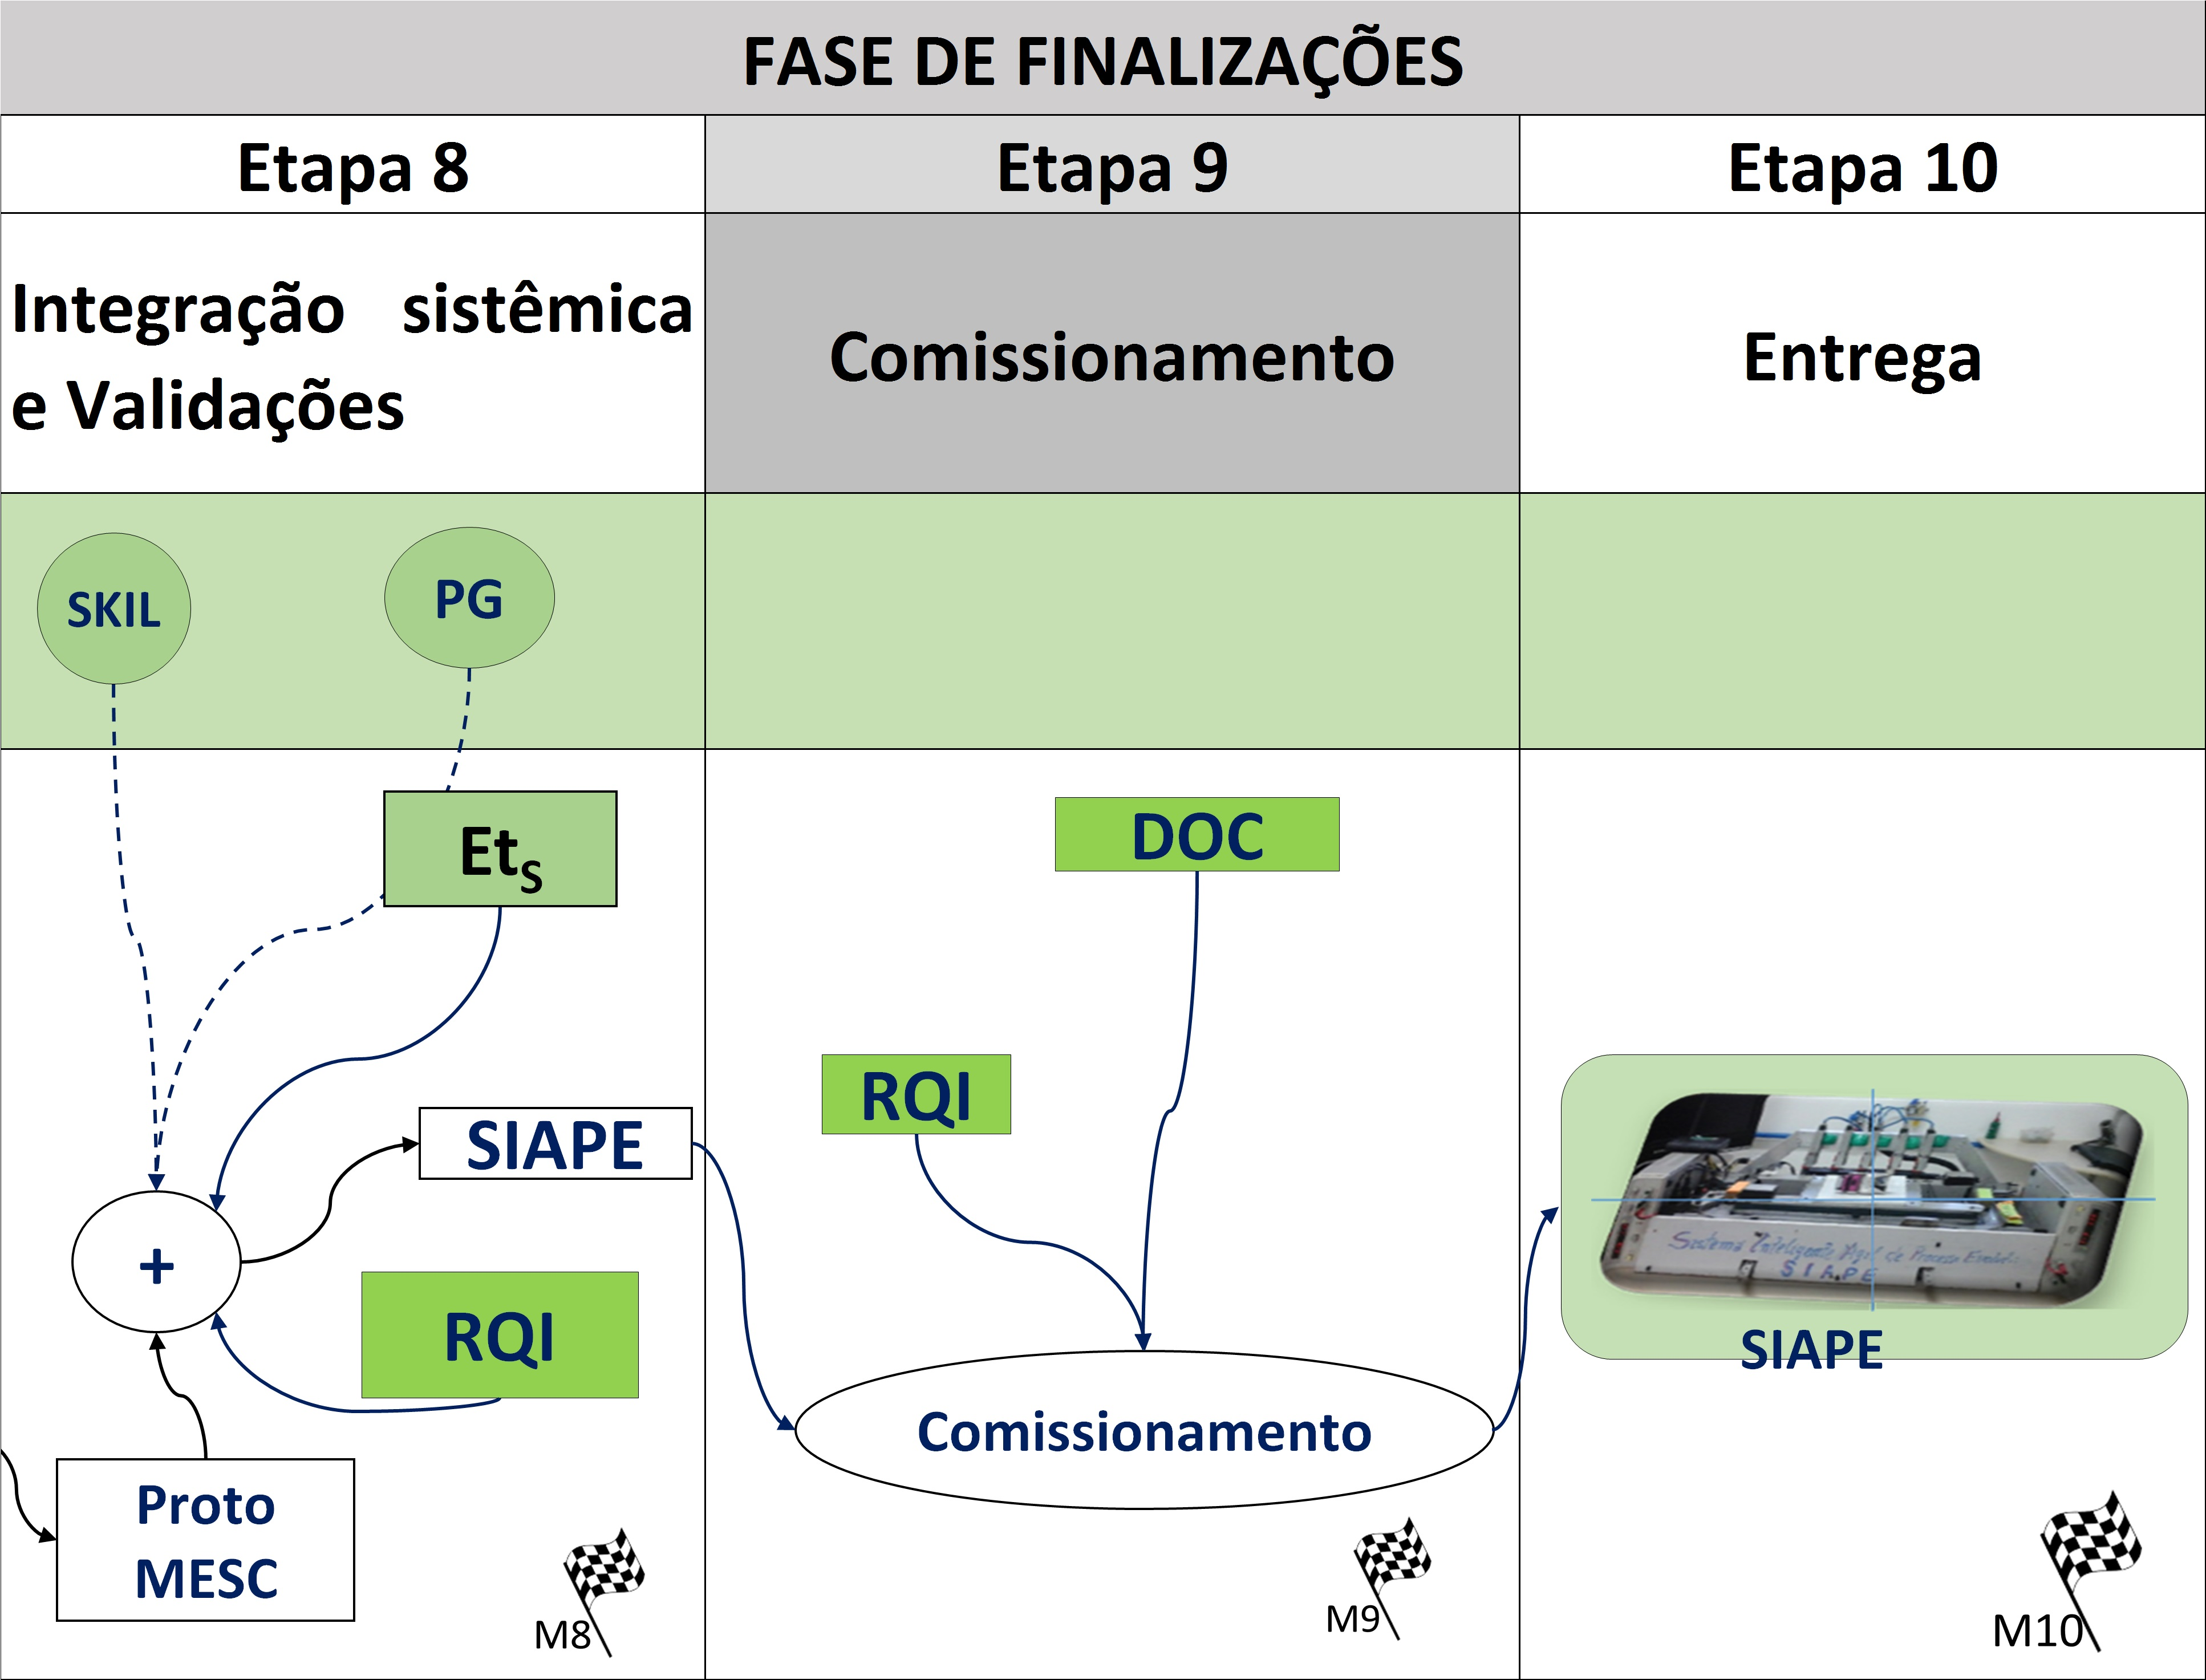
\includegraphics[width=10cm, height=5cm]{F27_2_SIAPE_FINALIZACOES.jpg} 
	\caption{MeDSE: Fase de Finalizações}
	\label{F27_2}
\end{figure}
 
\begin{description}
 	
 	\item[Etapa 8 - Integração e validação sistêmica] - Nesta fase o sistema modular integrado na Etapa 7 é submetido ao processo de integração sistêmica para que seja validado contra os RQI e contra as Ets. Nesta fase o sistema é solicitado a realizar um pedido de usuário que represente uma situação normal de produção. A realização do pedido evidenciará, neste projeto, as atividades dos agentes inteligentes mecatrônicos que se utilizam de seus \textit{skills} para atingir as metas impostas pelo usuário (a realização do pedido). Ao final deste processo têm-se o SIAPE que representa a solução para o problema global identificado pela equipe de desenvolvimento, e que atende aos requisitos do solicitados pelo cliente. 
 	
 	\item[Etapa 9 - Comissionamento] - Na Etapa 9 a documentação técnica, e do usuário, é finalizada e o sistema é comissionado contra o manual de operação técnica, e contra o manual de usuário. É importante notar, que mesmo nesta etapa, os registros que identificam se as metas foram alcançadas utilizam-se dos RQI para elucidar qualquer potencial inconsistência surgida. 
 	
 	\item[Etapa 10 - Entrega] - Na Etapa 10 o sistema é demonstrado ao cliente e entregue oficialmente, encerrando a fase de desenvolvimento. Na comparação ilustrada na Figura \ref{F13_1},  \citeonline{RUMBAUGH2006} propõe, após a implantação, a fase de manutenção do sistema. Como o foco desse trabalho de pesquisa é o de sistemas evolutivos, a fase de manutenção faz parte da evolução e adaptação do sistema e é realizada pela equipe de desenvolvimento de acordo com o tempo definido em contrato para esse fim.  
\end{description}
 	
 	
%================================ APLICAÇÃO DO MEDSE AO SIAPE =================================
\cleardoublepage
\section{Aplicação do MeDSE ao SIAPE}

Esta seção descreve a aplicação do MeDSE na realização do SIAPE, por meio das descrições dos procedimentos práticos realizados no desenvolvimento de cada etapa do método. Para que a descrição reflita os passos e facilite entendimento dos mesmos,  cinco itens foram definidos e encontram-se ilustrados na Tabela~\ref{T2}. 

%===============================

\begin{table}[htb]
	\center
	\footnotesize
	\begin{tabular}{|p{1.4cm}|p{1cm}|p{3cm}|p{3cm}|}
		\hline
		\textbf{Folha} & \textbf{Linha}  & \textbf{Onde se lê}  & \textbf{Leia-se}  \\
		\hline
		1 & 10 & auto-conclavo & autoconclavo\\
		\hline
	\end{tabular}
\end{table}
%----------------------------------

\begin{table}[h]
	\centering
	\caption{Itens processados em cada etapa}
	\begin{tabular}{|l| p{13.5cm}| c| c| } \hline
		\textbf{ Item} 	   & \textbf {Descrição}	 \\ \hline
		\textbf{1.Objetivos}   & Descrição do objetivo da etapa \\ \hline
		\textbf{2.Entradas}	   & Identificação das entradas no processo de transformação da etapa  \\ \hline
		\textbf{3.Processo }    & Processo que transforma as entradas em saídas \\ \hline
		\textbf{4.Saídas}		  & Resultado da realização do processo de transformação. Igual ao marco da etapa\\ \hline
		\textbf{5.Registros}	 & Documentos gerados na etapa e, se necessário geram realimentações \\ \hline
	\end{tabular}
	\label{T2}
	%	Fonte: Hiram Amaral
\end{table}

Essa tabela é utilizada no procedimento padrão adotado para descrever as etapas, e este foi seguido durante todo o desenvolvimento do SIAPE. A Figura \ref{F50} ilustra o procedimento que é dividido em duas parte e sua explicação é feita a seguir:

\begin{description}
	\item[Primeira parte] - Em todas as etapas os cinco itens definidos  são descritos numa tabela;
	\item[Segunda parte] - A etapa é descrita textualmente, e onde aplicável, figuras são ilustradas. 
\end{description}


 \begin{figure}[h]
 	\centering
 	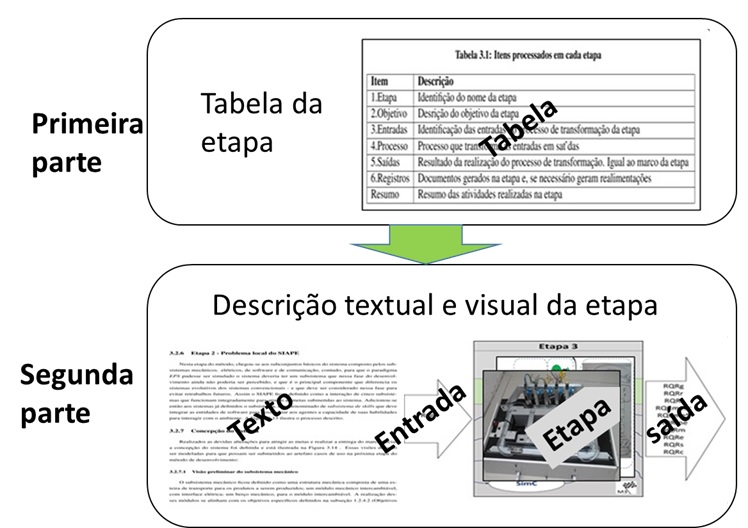
\includegraphics[width=8cm, height=5cm]{F50_MEDSE_2FORMAS1.jpg} 
 	\caption{MeDSE: Descrição da atividades nas etapas}
 	\label{F50}
 \end{figure}


 A descrição textual e visual da etapa expande, resumidamente, os títulos relacionados na tabela. A visualização evidencia pontos relevantes através de fotos, diagramas, esquemas ou figuras. \par 

%=================================================

Realizadas as explanações sobre o MeDSE e definido o procedimento padrão, espera-se que o projetista esteja habilitado para seguir a aplicação do  MeDSE e realizar o SIAPE.
\cleardoublepage
%++++++++++++++++++++++++++++++++++++++++++++++++++++++++++++++++++++++++++++++++++++++++++++++++++++++++++++++
\subsection{ETAPA 1 - CONCEITOS}

\begin{description}

\begin{table}[htbp]
	\centering
	\caption{Tabela da etapa 1 - Conceitos}
	%=================================================================================================
	\begin{tabular}{|l| p{13.5cm}| c| c| } \hline
		%================================================================================================
		\textbf {Item} 	   & \textbf {Descrição}	 \\ \hline
		%================================================================================================
		\textbf{1. Objetivos} &  
		Elaborar a concepção do sistema\\ \hline
		%================================================================================================
		\textbf{2. Entradas}  &		 
		1 -- As necessidades do cliente\par  	
		2 -- Referenciais específicos do Paradigma EPS\par 	
		3 -- Referenciais externos relacionados ao sistema  \\ \hline	
		%================================================================================================	
		\textbf{3. Processo}    & Gerar requisitos \\ \hline
		%================================================================================================
		\textbf{4. Saídas}	     & 
		Documento de Concepção do sistema contendo os requisitos iniciais (RQI) e o problema global (PG)\\ \hline
		%================================================================================================		
		\textbf{5. Registros}	& 	
		1 --Documento de Concepção do sistema \par
		2 -- Diagrama de Requisitos Pai \par
		3 -- Diagrama de Requisitos filhos\\ \hline
		%================================================================================================
	\end{tabular}
	\label{T3}\par
	%	Fonte: Hiram Amaral
\end{table}

\item[Descrição textual e visual da etapa] - Os conceitos, requisitos e restrições foram esquematizados para que o Problema Global fosse elaborado, A Figura \ref{F62} ilustra a sintetização que gerou o Problema Global (PG).  O PG também pode ser representado pelas partes do sistema M, E, S, C e SK (Skills).


\end{description}

\begin{figure}[!h]
	\centering
	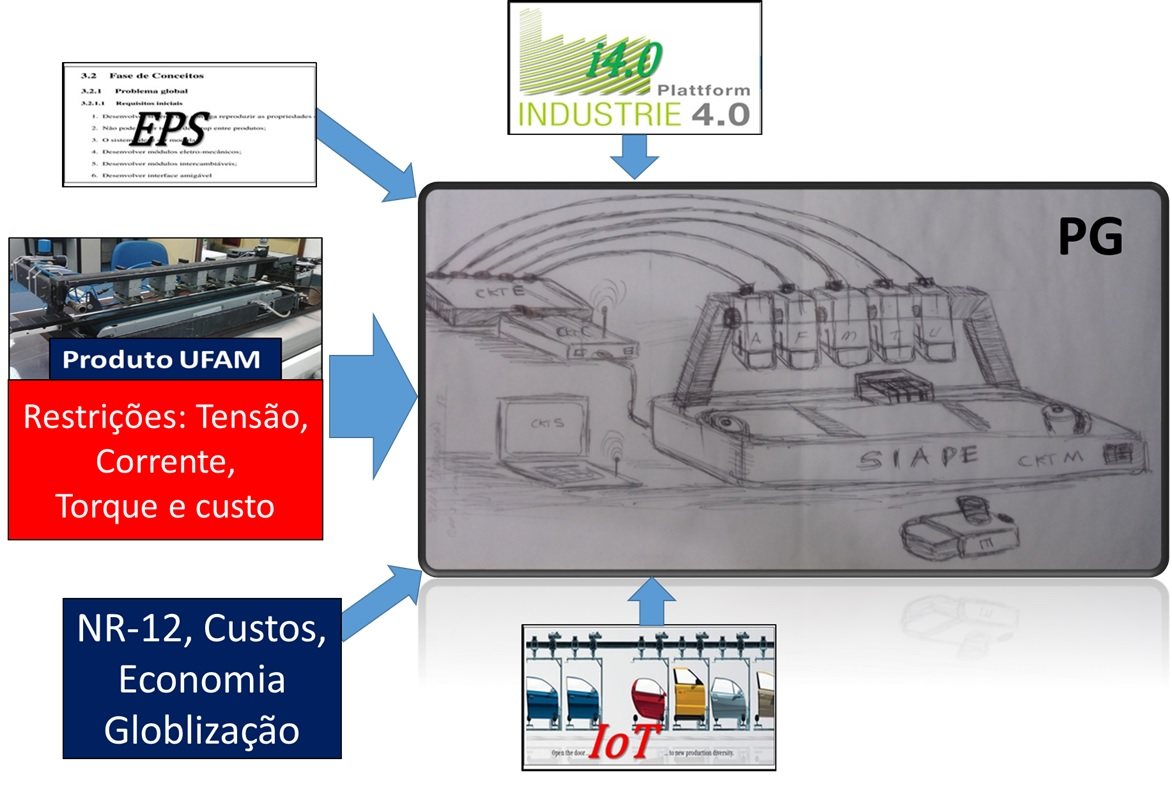
\includegraphics[width=14cm, height=8cm]{F62_SIAPE_PG.jpg} 
	\caption{SIAPE: Problema Global}
	\label{F62}
\end{figure}
Para desenvolver a concepção do sistema, as necessidades do cliente são consideradas, a saber:\par   	
a.	Desenvolver um sistema que consiga expressar as características dos sistemas evolutivos e evidenciar potenciais capacidades para reduzir o problema da customização de massa. Além disso, o sistema deve considerar alguma recomendações da Plataforma da Indústria 4.0 (i4.0) e capturar algum conceito da arquitetura Internet das Coisas (IoT) no tocante Manufatura Ágil. \par 
b.	O sistema deve ser baseado no Produto UFAM com as devidas alterações de melhorias; \par 
c.	O sistema deve carimbar as 5 letras A, F, M, T  e U; \par 
d.	Deverá ser criado um módulo para letra que seja exigido em nova palavra; \par 
e.	O sistema de carimbar as palavras UFAM, UTAM e UEA; \par 
f. O sistema deveria ser baseado no Produto UFAM.\par
Somam-se às necessidades do cliente, os referenciais específicos do Paradigma \textit{EPS}. Das características básicas do Paradigma \textit{EPS} extraiu-se capacidade de \textit{adaptação}, implicando que o sistema deve ser capaz de propor uma alternativa de configuração para minimizar os efeitos de perturbarções externas, e a capacidade de \textit{evolução}, implicando que o sistema deve ser capaz de aceitar a troca de módulos em tempo de produção. \par 

Para realizar as principais características as propriedades da Modularidade, Granularidade, Plugabilidade e Reconfigurabilidade devem estar presente no sistema.\par 
%\textbf{Modularidade}: a noção de módulos independentes devem estar presente no sistema EPS. \par  
\ %textbf{Plugabilidade:} A capacidade de lidar com a introdução de novos módulos, enquanto o sistema está funcionando. O sistema deve ser capaz de redesenhar a dinâmica %interna, a fim de manter a sua eficiência. \par  
%\textbf{Reconfigurabilidade:} O sistema precisa ser capaz de lidar com o redesenho do layout sem comprometer qualquer funcionalidade.
	
Além dos referenciais do cliente e de EPS são considerados os referenciais externos relacionados ao sistema:	 \par 
\textbf{Academia} - O sistema deve refletir o estado da arte em paradigmas de manufatura.\par 
\textbf{Globalização} -  O sistema deve evidenciar potenciais soluções para a questão da customização de massas.\par 
\textbf{Indústria 4.0} - A integração horizontal definida como a agregação, em tempo real dos elementos de sistemas no chão--de--fábrica, relacionando a comunicação, o planejamento e a programação desses sistemas, contendo elementos que serão usados para incorporar raciocínio baseado em casos de uso, evidenciando a capacidade de evoluir com a mudança dos requisitos de produção, deverá estar presente no sistema.\par 
\textbf{Internet das Coisas} -  O conceito plugar e trabalhar \textit{ Plug \& Work}  é definido como a capacidade de dispositivos e componentes de rede para auto-configurar-se de acordo com as necessidades das aplicações da automação. \textit{Plug \& Work} deve trabalhar em ambientes 4.0 e reduzir maciçamente as ações manuais e reduzirá tanto o tempo de inatividade global quanto o número de erros do sistema.\par 
\textbf{Governo} -  Para atender a exigência de segurança, o governo editou a Norma Regulatória número 12 (NR-12) que de acordo com o item 12.56, as máquinas devem ser equipadas com um ou mais dispositivos de parada de emergência, por meio dos quais possam ser evitadas situações de perigo latentes e existentes.\par 
\textbf{Economia} -  Por meio da redução de custos no processo produtivo incrementa-se o nível de competitividade dos produtos originados nesse processo. Portanto, as vantagens comparativas entre o SIAPE e os sistemas de produção vigentes tendem a se transformar em ganhos de competitividade, e deverão ser mensurados e quantificados no processo evolutivo. \par 
As necessidades do cliente, os referenciais internos e os referenciais externos foram sintetizados na geração dos RQI conforme ilustra a Figura \ref{F61}. 

\begin{landscape}
	\begin{figure}[!h]
		\centering
		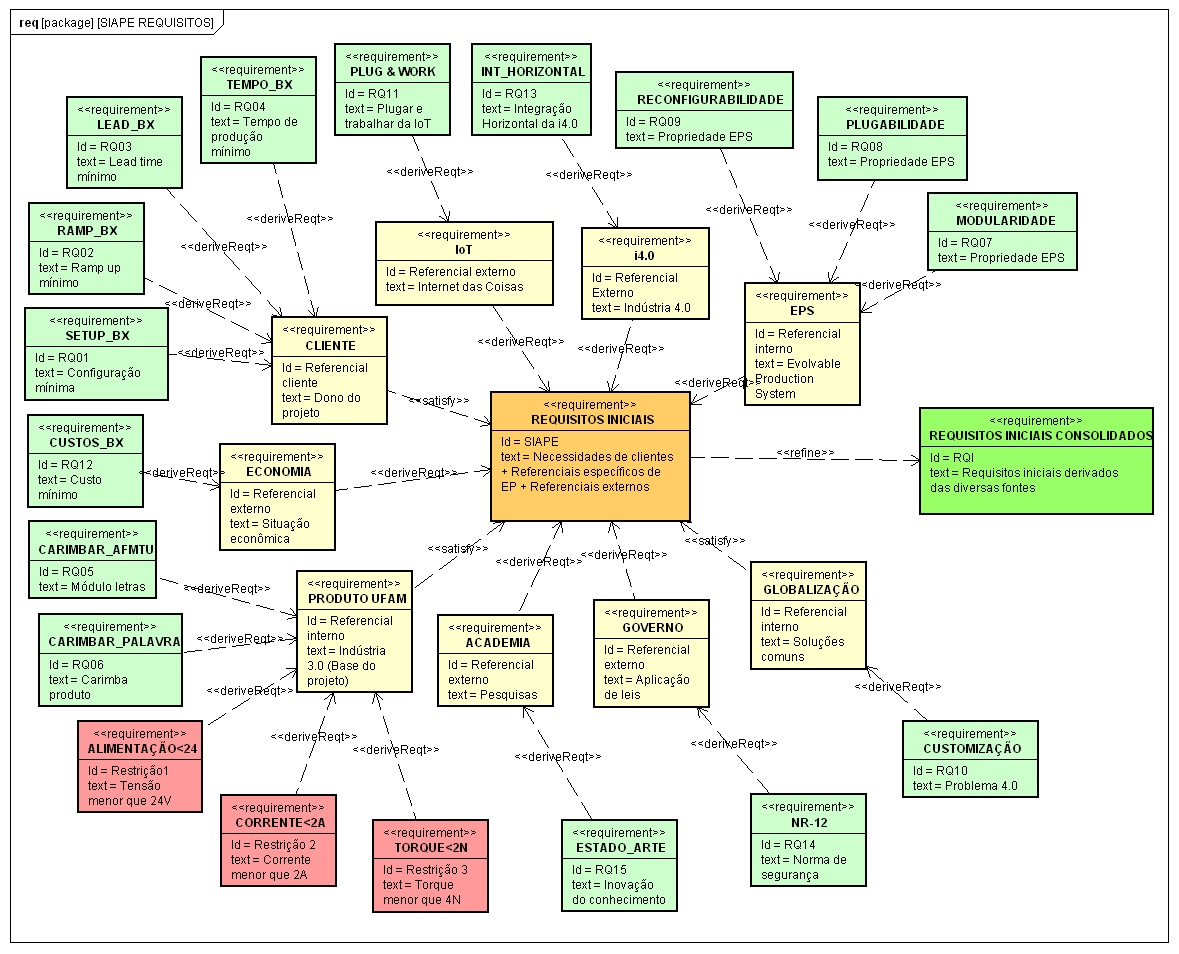
\includegraphics[width=24cm, height=14cm]{F61_SIAPE_REQUISITOS_V03.jpg} 
		\caption{SIAPE: Requisitos}
		\label{F61}
	\end{figure}
\end{landscape}


A Figura \ref{F61} ilustra  o processo de agregação dos requisitos do sistema em tipos de requisitos. Tais agregações são filtradas produzindo em sua saída uma relação de requisitos, denominados de requisitos iniciais que serão submetidos ao processamento da próxima etapa. 

Na saída do processo têm-se o Documento de Concepção do sistema contendo os requisitos iniciais (RQI) e o problema global (PG).

A ilustração da Figura \ref{F64}  detalha a visão da concepção do sistema. Nesta figura está montado o cenário para as verificações e validações finais realizadas na Fase de Finalizações do método de desenvolvimento. Quando um pedido é realizado por clientes, estes pedidos são inseridos por um operador na Interface Homem Máquina (IHM). A partir da inserção dos pedidos na IHM, o agente Order solicita ao agente YPA os nomes dos módulos que estão presentes no sistema. Com a informação fornecida o agente Order cria o plano de produção e envia ao agente Anagrama. O Anagrama realiza o plano enviando os comandos ao agente AcHw (Acesso Hardware). O AcHw envia os comando através do \textit {Raspberry Pi} à parte elétrica, que ativa os atuadores e realiza os produtos solicitados pelos clientes. O operador entrega os produtos a seus respectivos clientes e o ciclo se fecha.     

\begin{figure}[!h]
	\centering
	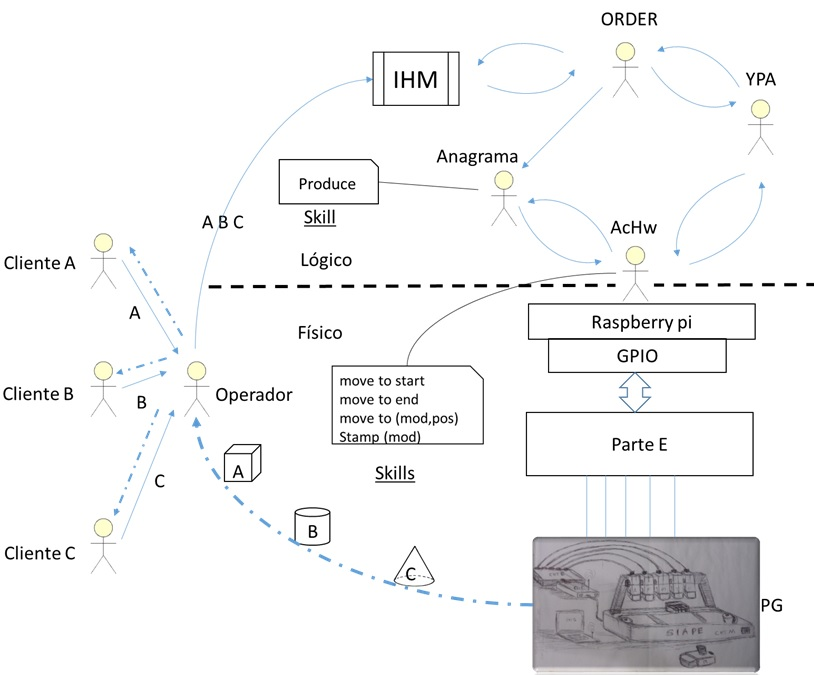
\includegraphics[width=16cm, height=10cm]{F64_SIAPE_VISAO_CONCEPCAO_SISTEMA.jpg} 
	\caption{SIAPE: Cenário concepção do sistema}
	\label{F64}
\end{figure}


O entendimento das funções de parte do sistema é fundamental para a realização da Etapa~2. Para compatibilizar  alguns parâmetros entre Produto UFAM e SIAPE foi assumido como restrição que a alimentação máxima do sistema deveria ser <~24V, com uma corrente <~2A e um custo máxima da ordem de dez vezes o valor investido no Produto UFAM. 

Os RQI e o PG originaram o documento de Concepção do Sistema que contém as informações de entrada para a próxima etapa. A Figura \ref{F63} ilustra a inclusão do RQI e PG no documento de Concepção do Sistema SIAPE e evidencia a realização do segundo marco: Entrega do Documento de Concepção do Sistema.

\begin{figure}[!h]
	\centering
	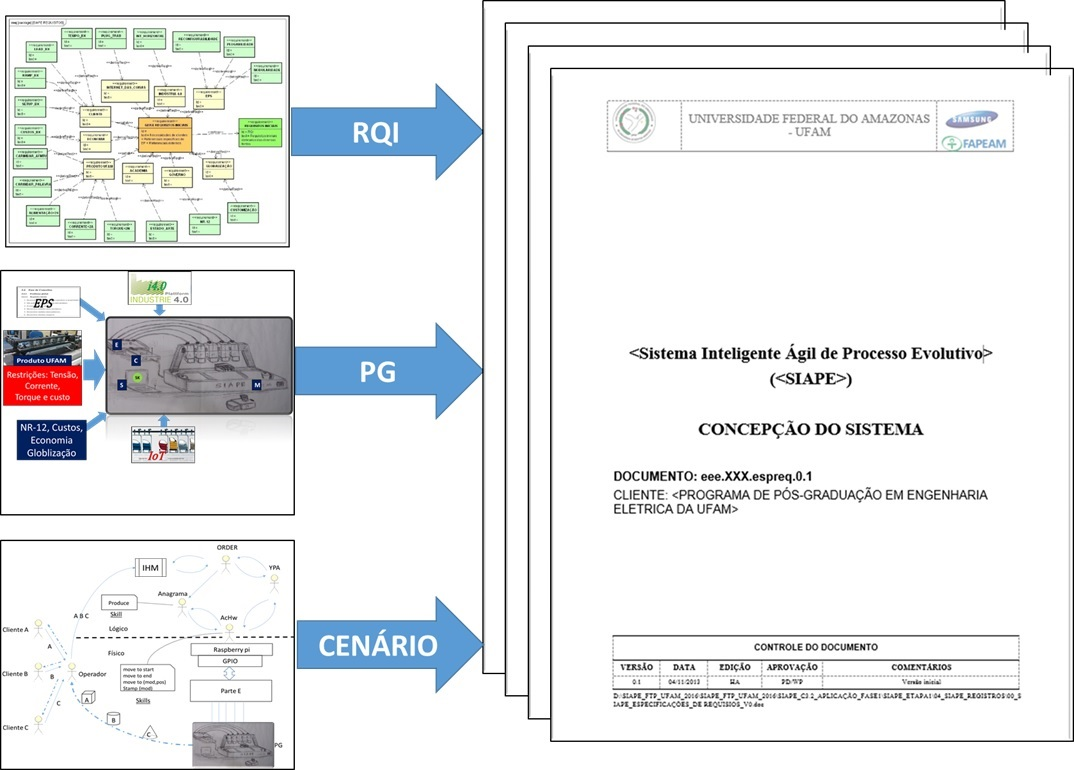
\includegraphics[width=16cm, height=10cm]{F63_SIAPE_CONCEPCAO_SISTEMA.jpg} 
	\caption{SIAPE: Geração do documento de concepção do sistema}
	\label{F63}
\end{figure}

Ao entregar o Documento de Concepção do Sistema contendo os Requisitos Iniciais (RQI), a definição do Problema Global (PG) e o Cenário que deverá ser utilizado para validar o sistema (na Fase de Finalizações), o objetivo da etapa é atingido.


\cleardoublepage
  %+++++++++++++++++++++++++++++++++++++++++++++++++++++++
\subsection{ETAPA 2 - ANÁLISES}
\begin{description}
\begin{table}[htbp]
	\centering
	\caption{Tabela da etapa 2 - Análises}
	%=================================================================================================
	\begin{tabular}{|l| p{13.5cm}| c| c| } \hline
		%================================================================================================
		\textbf{Item} 	    & \textbf{Descrição} 
		\\ \hline
		%================================================================================================
		\textbf{1.Objetivo}	   &  
		Refinar os requisitos inciais do cliente (RQI)\\ \hline
		%================================================================================================
		\textbf{2.Entradas}	  &		
		Documento de Concepção do sistema contendo os requisitos iniciais (RQI) e o problema global (PG)\par  	
		\\ \hline	
		%================================================================================================	
		\textbf{3.Processo}     &
		Refinar RQI\\ \hline
		%================================================================================================
		\textbf{4.Saídas}		& 
		Requisitos refinados (RQR): RQRmesc, RQRmes, RQRme, RQRm, RQRe, RQRs, RQRc, RQRa, RQRf, RQRm, RQRt RQRu 
		\\ \hline
		%================================================================================================		
		\textbf{5.Registros}   & 	
		Planilha de requisitos refinados do sistema\\ \hline
		%================================================================================================
	\end{tabular}
	\label{T4}\par
	%	Fonte: Hiram Amaral
\end{table}

\item[Descrição textual e visual da etapa] - A Etapa de Análises tem o objetivo de refinar os requisitos inicias e especificá-los para cada parte do Problema Global em sua forma MESC. \par 
Os requisitos iniciais (RQI) e o problema global (PG) contidos no Documento de Concepção do Sistema são divididos para serem refinados. 	O Problema Global (PG) é convenientemente dividido em Problema Regional (PR) e Problema Local (PL) e são relacionados com as partes do sistema mecatrônico MESC: MESCmain, MES, ME, M, E, S, C, MESCA, MESCF, MESCM, MESCT e MESCU e MESCE. Onde:

\item[Definição dos agentes baseada na Arquitetura SIAPE] - Para a definição da quantidade e do tipo de agentes a serem utilizados na proposta de solução ao PG foram definidos os seguintes agentes da arquitetura aserem implementados:

\begin{description}
	\item[01 YPA ]- Para registrar os agentes existentes na plataforma e buscar seus \textit{skills}.	
	\item[01 OrderAgent] - Com a função de\textit{GATEWAY} para a interface homem máquina do EPS e instanciar os anagramas de acordo com a ordem de serviço gerada na IHM.	
	\item[01 Anagram] - Para representar os produtos (ANAGRAMA) a serem produzidos.
	\item[01 AcHw] - Para detectar e informar os módulos disponíveis no sistema.
	\item[01 Conveyor] - Para representar a ESTEIRA do sistema que realizar o transporte dos produtos.	
	\item[01 Stamper] - Para representar os MÓDULOS CARIMBADORES do sistema e carimbar as letras do anagrama na palete.
\end{description}
\end{description}

	A Figura \ref{F145} mostra os agentes da arquitetura SIAPE aplicados ao caso do PG. Essa aplicação, neste momento do desenvolvimento, torna-se necessária para evidenciar um exemplo prático da arquitetura que foi implementado neste etapa, e experimentado e validado nos Capítulos 4 e 5.
	
	\begin{figure}[h]
		\centering
		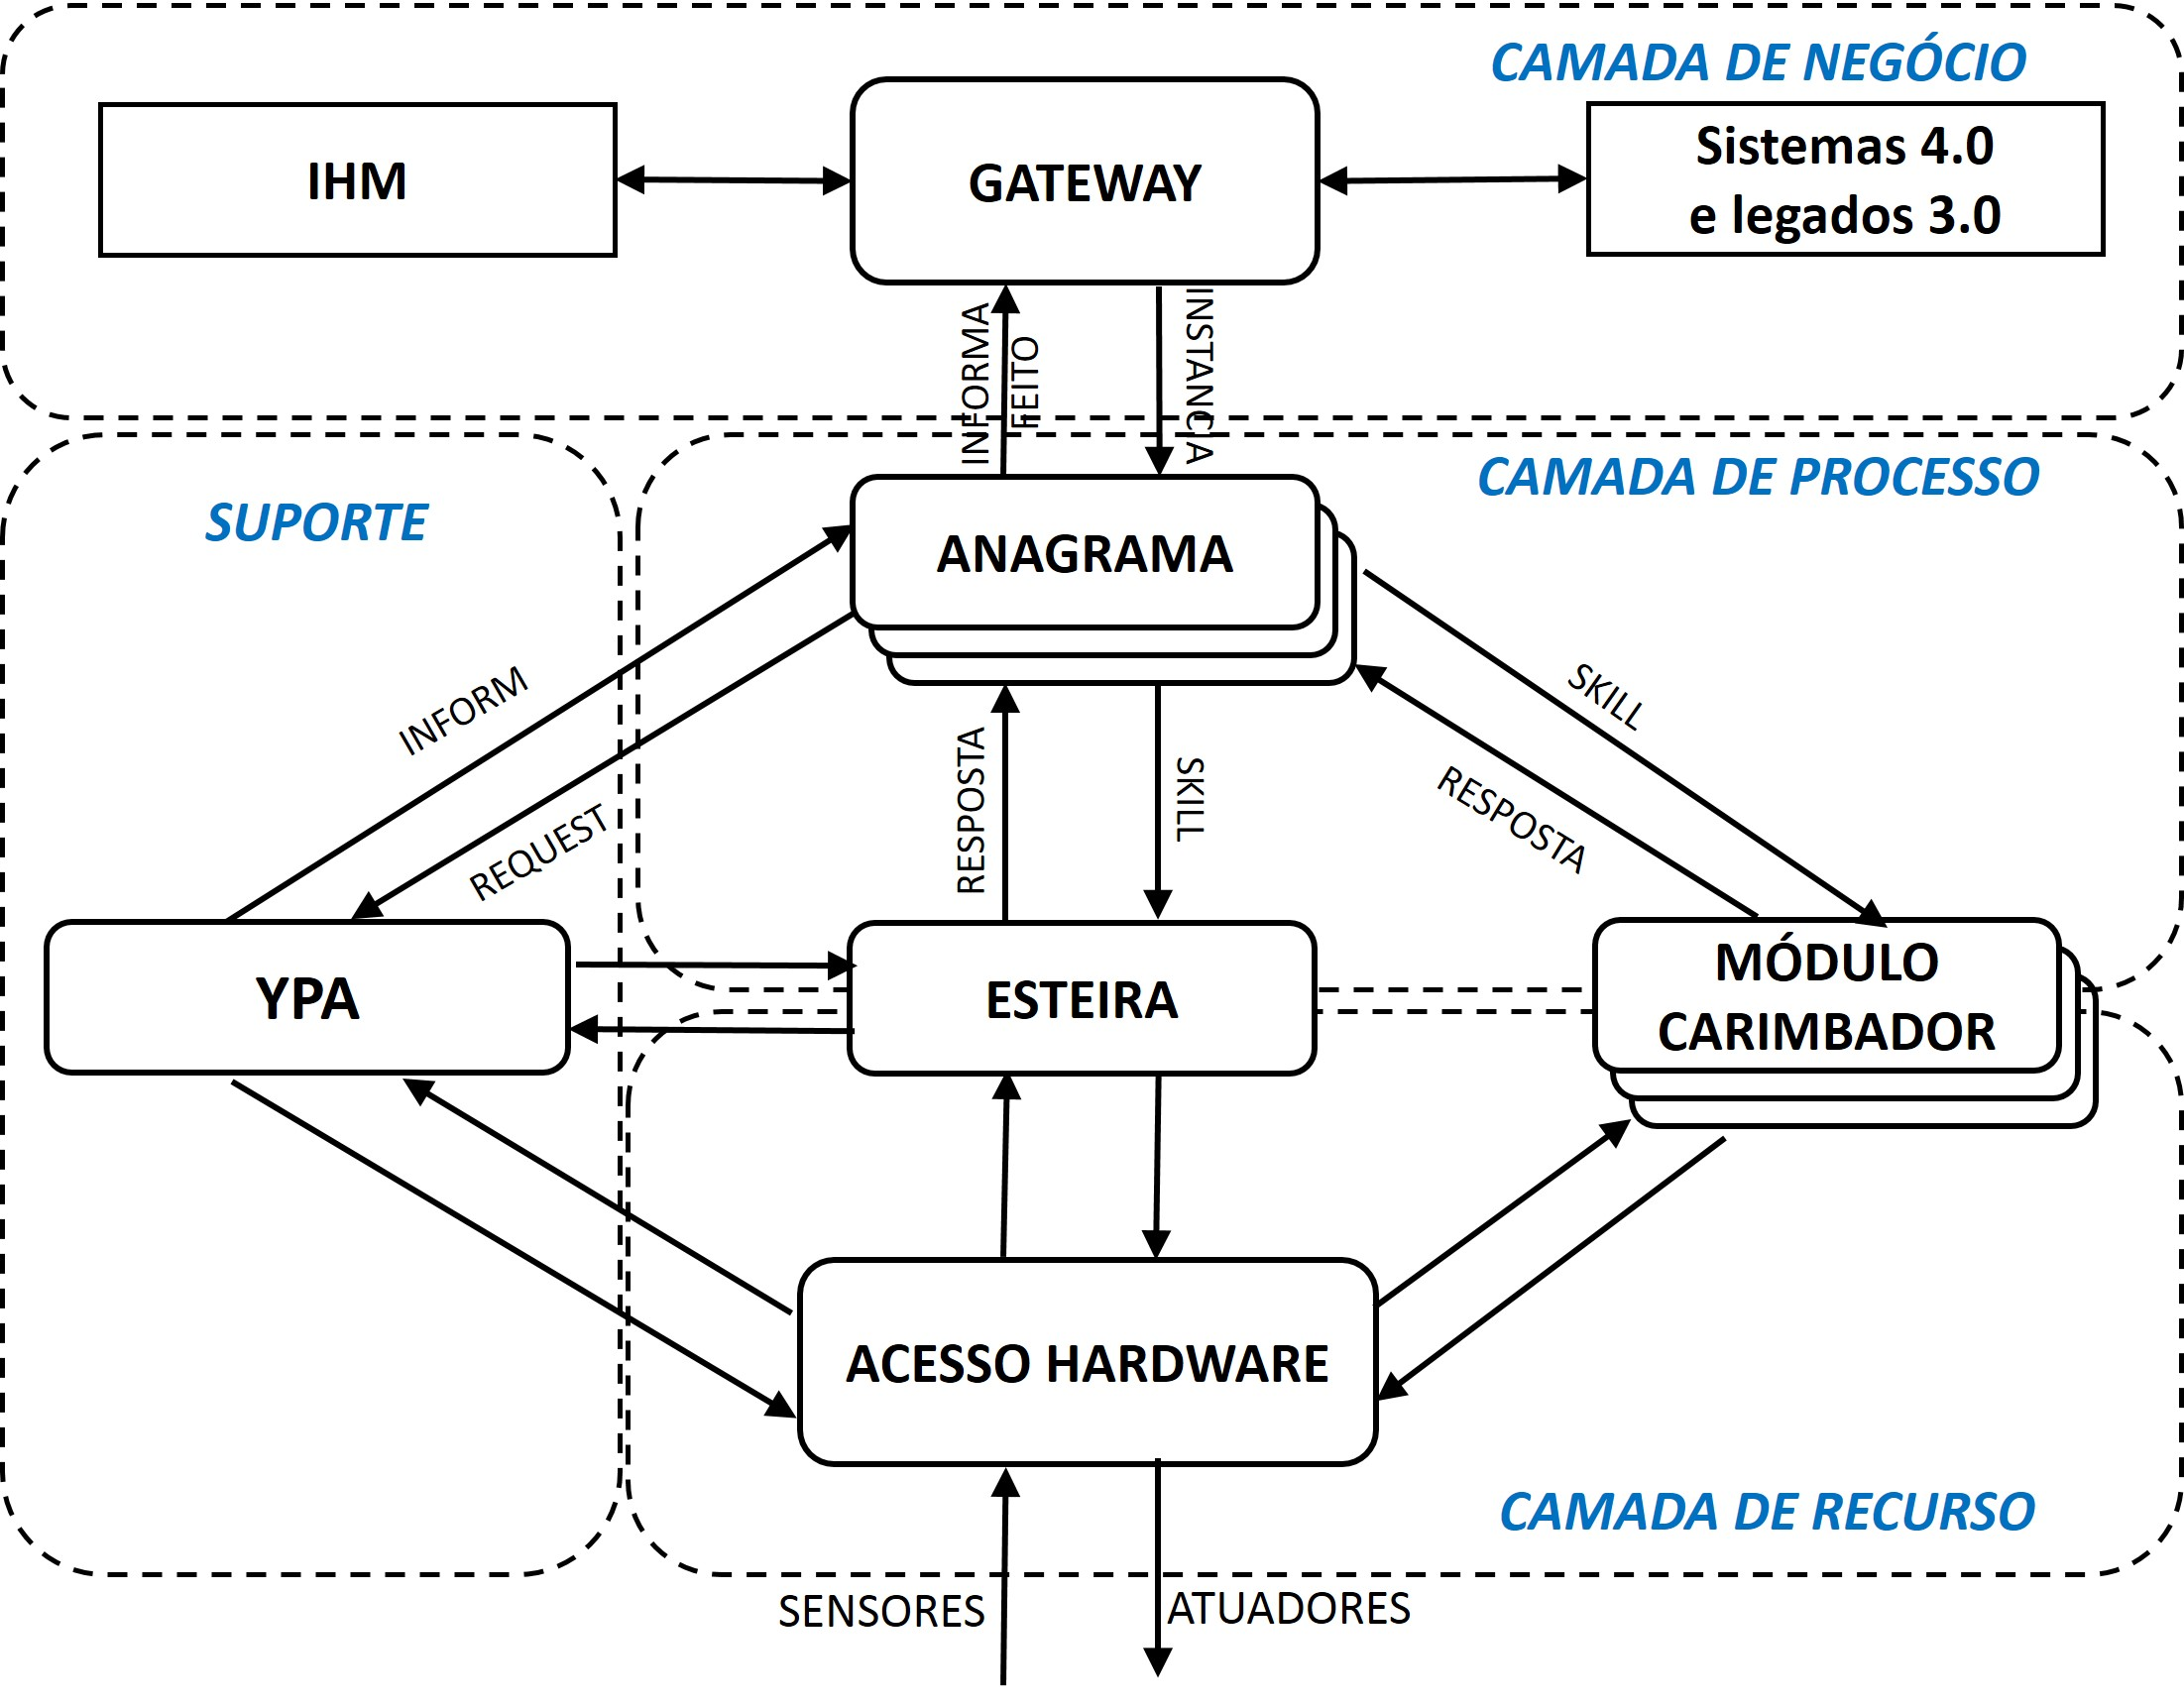
\includegraphics[width=12cm, height=9cm]{F144_arquitetura_PG.jpg} 
		\caption{SIAPE: Arquitetura SIAPE aplicada ao PG}
		\label{F145}
	\end{figure}

	\begin{description}
			\item[MESCmain] - representa a parte do MESC principal  do sistema contendo a integração das partes M, E, S e C e tem seus requisitos refinados e rotulados como RQRmesc;
			\item[MES] - representa a parte do MESC contendo a integração das partes M, E e S do MESC principal e tem seus requisitos refinados o rotulados como RQRmes;
			\item[ME] - representa a parte ME do MESC contendo a integração das partes M e E e tem seus requisitos refinados e rotulados como RQRme;
			\item[M] - representa a parte mecânica do MESC principal e tem seus requisitos refinados e rotulados como RQRm;
			\item[E] - representa a parte eletrônica do MESC principal e tem seus requisitos refinados e rotulados como RQRe;
			\item[S] - representa a parte de software do MESC principal e tem seus requisitos refinados e rotulados como RQRs;
			\item[C] - representa a parte comunicação do MESC principal e tem seus requisitos refinados e rotulados como RQRc;
			\item[MESCa] - representa o módulo mecatrônico que realiza a letra A e  tem seus requisitos rotulados como RQRA;
			\item[MESCf] - representa o módulo mecatrônico que realiza a letra F e  tem seus requisitos rotulados como RQRF ;
			\item[MESCm] - representa o módulo mecatrônico que realiza a letra M e  tem seus requisitos rotulados como RQRM; 
			\item[MESCt] - representa o módulo mecatrônico que realiza a letra T e  tem seus requisitos rotulados como RQRT;
			\item[MESCu] - representa o módulo mecatrônico que realiza a letra U e  tem seus requisitos rotulados como RQRU;
			\item[MESCe] - representa o módulo mecatrônico que realiza a letra E e  tem seus requisitos rotulados como RQRE.		
	\end{description}
	
O resultado na  saída do processo é o conjunto de documentos relacionados a seguir e que servem como registros das atividades realizadas. 	

		\begin{description}
			\item[MESCmain] - Documento de requisitos refinados do MESC principal;
			\item [RQRmes] - Documento de requisitos refinados das integrações MES e ME;
			\item[RQRm] - Documento de requisitos refinados da parte atômicas M, E, S e C do MESC principal;
			\item[RQRA] - Documento de requisitos refinados dos módulos mecatrônicos A, F, M, T, U e E;
		\end{description}

A Fase de Conceitos que realiza a Concepção do Sistema define uma ideia de sistema baseado na solicitação do cliente,  nas exigências internas, nas exigências externas e nas restrições. O segundo marco registra essa ideia por meio da entrega dos Requisitos Refinados. O conteúdo produzido até este momento deve ser confirmado, para que possa ser garantido como especificação e assumido como um projeto a ser realizado.  A Figura \ref{F65} ilustra os módulos de hardware e software que foram definidos para serem simulados ou verificados para que possam ser confirmados como especificações técnicas. \par 

\begin{figure}[h]
	\centering
	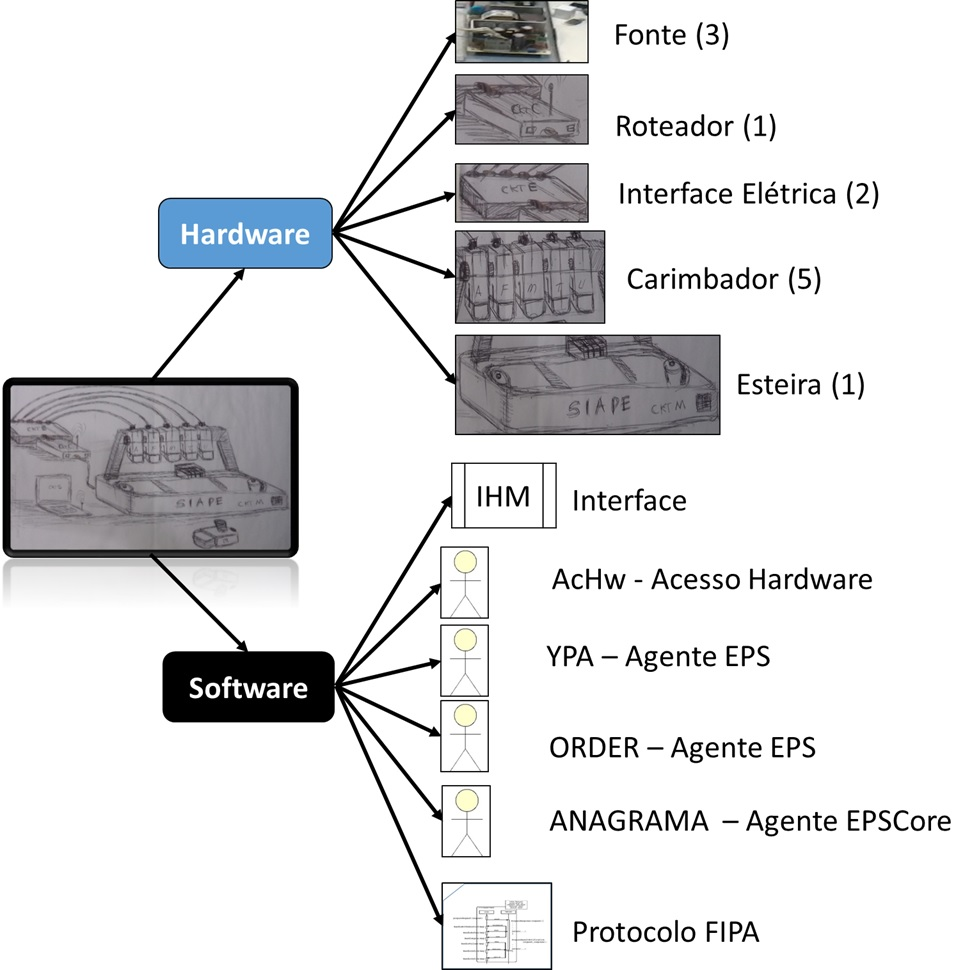
\includegraphics[width=12cm, height=12cm]{F65_SIAPE_HW_SW.jpg} 
	\caption{SIAPE: Módulos de Hardware e Software}
	\label{F65}
\end{figure}

Dos módulos definidos, três não precisaram ser modelados e simulados:

\begin{enumerate}
	\item Módulo Fonte, devido à restrição de 24V e 2A, foram adquiridas fontes que não ultrapassaram esses limites;
	\item Módulo Roteador por estar dentro da faixa de wireless de 2,4Ghz (B+G+N) com uma velocidade de 150 Mbps e uma potência de 700mW;
	\item Módulo Interface Elétrica devido à Placa Raspberry Pi Versão B+ ser aderente à linguagem de programação Java e, portanto, suportar o Framework Jade e compatível à Platafoma Linux. O único quesito não atendido pela Raspberry foi a quantidade de I/Os, e para resolver este problema tornou-se necessária a modelagem e desenvolvimento de uma extensão de I/Os. Essa extensão e os outros módulos encontram-se modelados e simulados na próxima etapa.\par 
\end{enumerate}


\newpage

%=================================== ETAPA 3 ==================================

\subsection{ETAPA 3 - SIMULAÇÕES}
 
Os documentos de requisitos refinados relacionam os Problemas Globais(PG), Regionais (PR) e Locais (PL) com os requisitos refinados. Esses documentos refinados servirão de base para a modelagem e simulação de todas as partes do MESC, a saber: RQRmesc, RQRmes , RQRme, RQRm, RQRe, RQRs, RQRc, RQRA, RQRF, RQRT, RQRU e RQRE. %são base para a a modelagem do sistema. \par 
 	 
As partes atômicas do MESC são submetidas ao processo de modelagem e depois ao processo de simulação. Após a realização desses processos o requisito pode ser aceito como especificação ou pode ser excluído da relação de  requisitos refinados. \par 
 	
Para melhorar o entendimento da visão definida na Etapa 2, com o objetivo de melhorar a realização do processo de modelagem, foi idealizado o caso de uso \textit{realizar um plano}, um diagrama de sequência, um diagrama de atividades e um diagrama de estados para o SIAPE. As Figuras \ref{F60}, \ref{F77}, \ref{F78}  e \ref{F79} ilustram, respectivamente, esses diagramas. Suas descrições encontram-se a seguir.
 	
A Figura \ref{F60} mostra o caso de uso ``Realizar Plano'', onde o Operador insere um pedido no sistema, o agente Order recebe o pedido e solicita informações ao agente YPA para a montagem do agente Anagrama responsável pelo processo produtivo do anagrama. O YPA responde ao Order, este monta o plano com o pedido e instancia o agente Anagrama. Este, por sua vez executa o plano realizando chamadas ao agente AcHw. O AcHw realiza as atividades, \textit{skill} a \textit{skill} e informa o término de cada qual ao Anagrama. O Anagrama, ao seu final, informa ao Order, e morre. O Order, por sua vez, confirma para o Operador a realização do pedido.

\begin{figure}[!h]
	 	\centering
	 	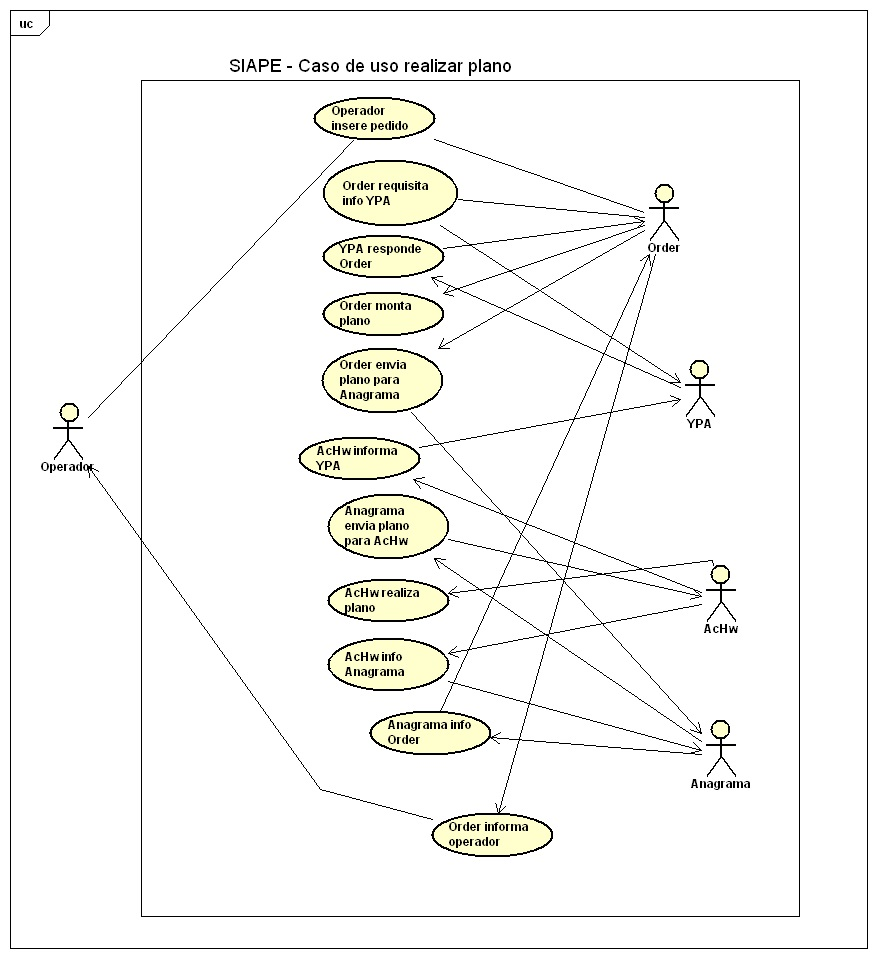
\includegraphics[width=14cm, height=12cm]{F60_SIAPE_CASUSO_PLANO.jpg} 
	 	\caption{Caso de uso: Realizar plano}
	 	\label{F60}
\end{figure}
 		 
A Figura \ref{F77} ilustra uma sequência do ponto de vista do operador. O Operador liga o sistema, o led vermelho é ligado. Em seguida o operador insere o pedido no sistema, carrega o palete na esteira e clica no botão de início de produção. O sistema liga a esteira. O sistema identifica a passagem do palete por meio do sensor, para a esteira e carimba o palete através do acionamento do atuador. Depois, volta a ligar a esteira e prossegue até o fim do plano. O sistema identifica o fim do plano e para a esteira. O operador retira o produto e desliga o sistema. 

\begin{figure}[!h]
 	 	\centering
 	 	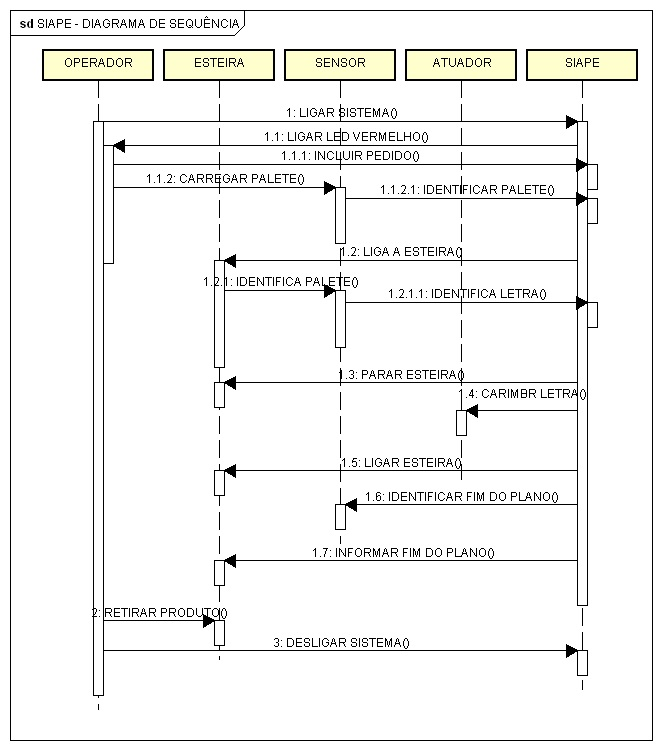
\includegraphics[width=14cm, height=10cm]{F77_SIAPE_DIAGRAMA_SEQUENCIA.jpg} 
 	 	\caption{SIAPE: Diagrama de sequência}
 	 	\label{F77}
\end{figure}
 		 	 
A Figura \ref{F78} ilustra o diagrama de atividades. Esse diagrama também auxilia no entendimento e desenvolvimento do software do sistema. É apenas uma outra visão para os mesmos procedimentos acima descritos. 
 		 	 
\begin{figure}[!h]
	\centering
	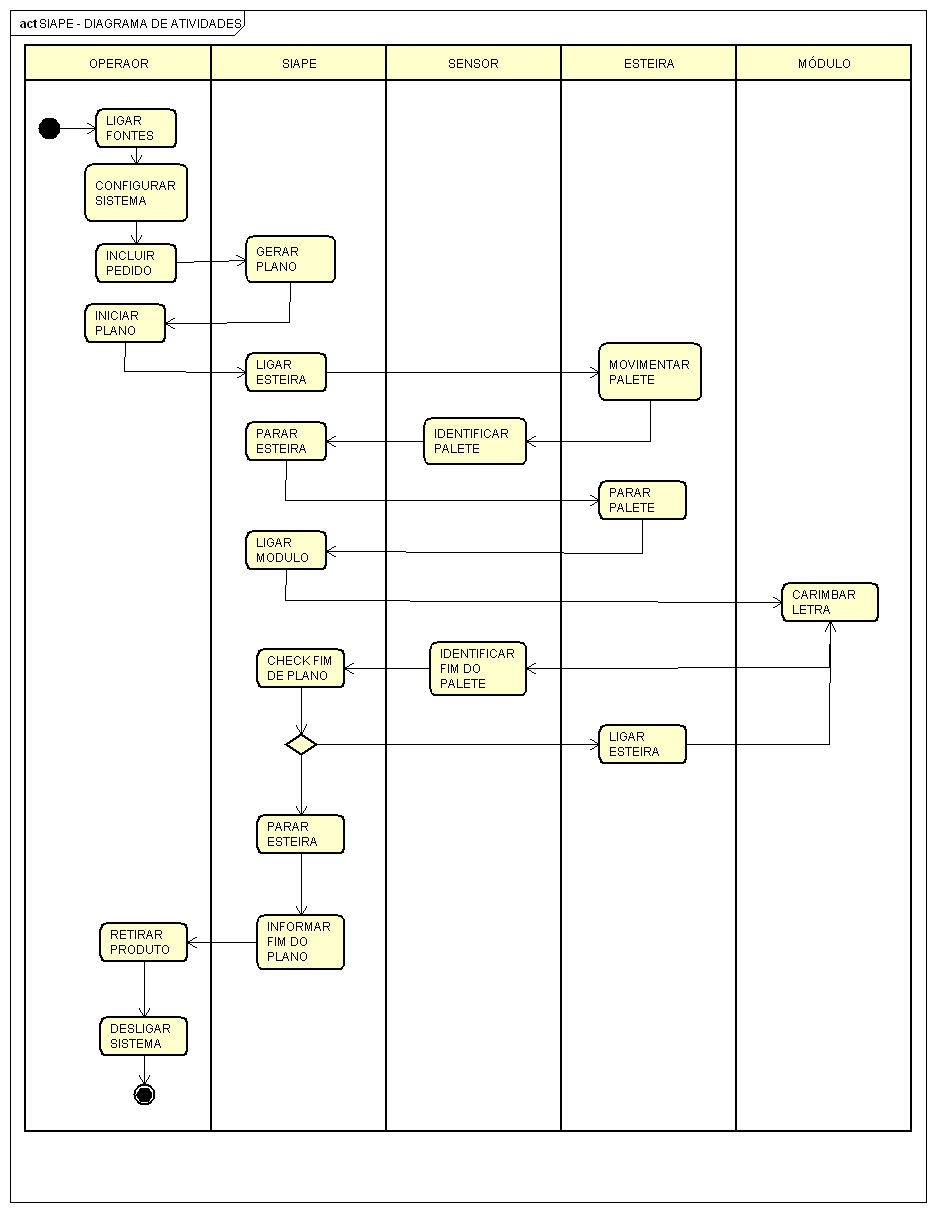
\includegraphics[width=14cm, height=14cm]{F78_SIAPE_DIAGRAMA_ATIVIDADES.jpg} 
	\caption{SIAPE: Diagrama de atividades}
	\label{F78}
\end{figure}
 		 	 	 
 		 	 	
 		 	 	 
 A Figura \ref{F79} ilustra o diagrama de estado do SIAPE que é baseado visão de OMAC para IEC 61131--3~ \cite{OMAC2006}, o qual descreve uma visão sistêmica e padronizada para equipamentos mecatrônicos, quer se trate de parte de uma linha de produção ou de uma máquina completa. Tal diagrama visa mostrar a funcionalidade e dinâmica do sistema.
 
 O diagrama de estado define completamente o estado corrente de uma máquina. As transições entre estados podem ser originados como resultado de uma intervenção  do operador, de uma resposta ao estado de um ou mais objetos de controle ou como resposta de modo completo, definido como a conclusão de todas as etapas que operam dentro de um estado definido. O processo é iniciado com a ligação do sistema e configuração dos dispositivos envolvidos na operação. Uma vez configurado, o sistema entra no modo inativo aguardando que o operador inclua um ou mais pedidos para que um plano de produção seja montado e disponibilizado para a produção. Uma vez que o plano é montado, entra no estado que é responsável por iniciar a produção do plano. O plano pode ser totalmente realizado ou pode ser suspenso para que se inicie outro plano, ou seja, suspenso para alimentação dos recursos de produção na linha. Havendo a suspensão o sistema, pode-se retornar no mesmo ponto de produção onde foi suspenso, ou reiniciado para o início de um novo plano. Também pode ser reiniciado evidenciando que o plano foi totalmente produzido e a operação trata-se de um novo plano sendo produzido. O diagrama também prevê a ocorrência de possíveis erros que são tratados por um processo que aborta a operação, limpa o sistema, pára o processo e uma nova operação pode ser iniciada.    
%
	 
\begin{landscape}
	\begin{figure}
		\centering
		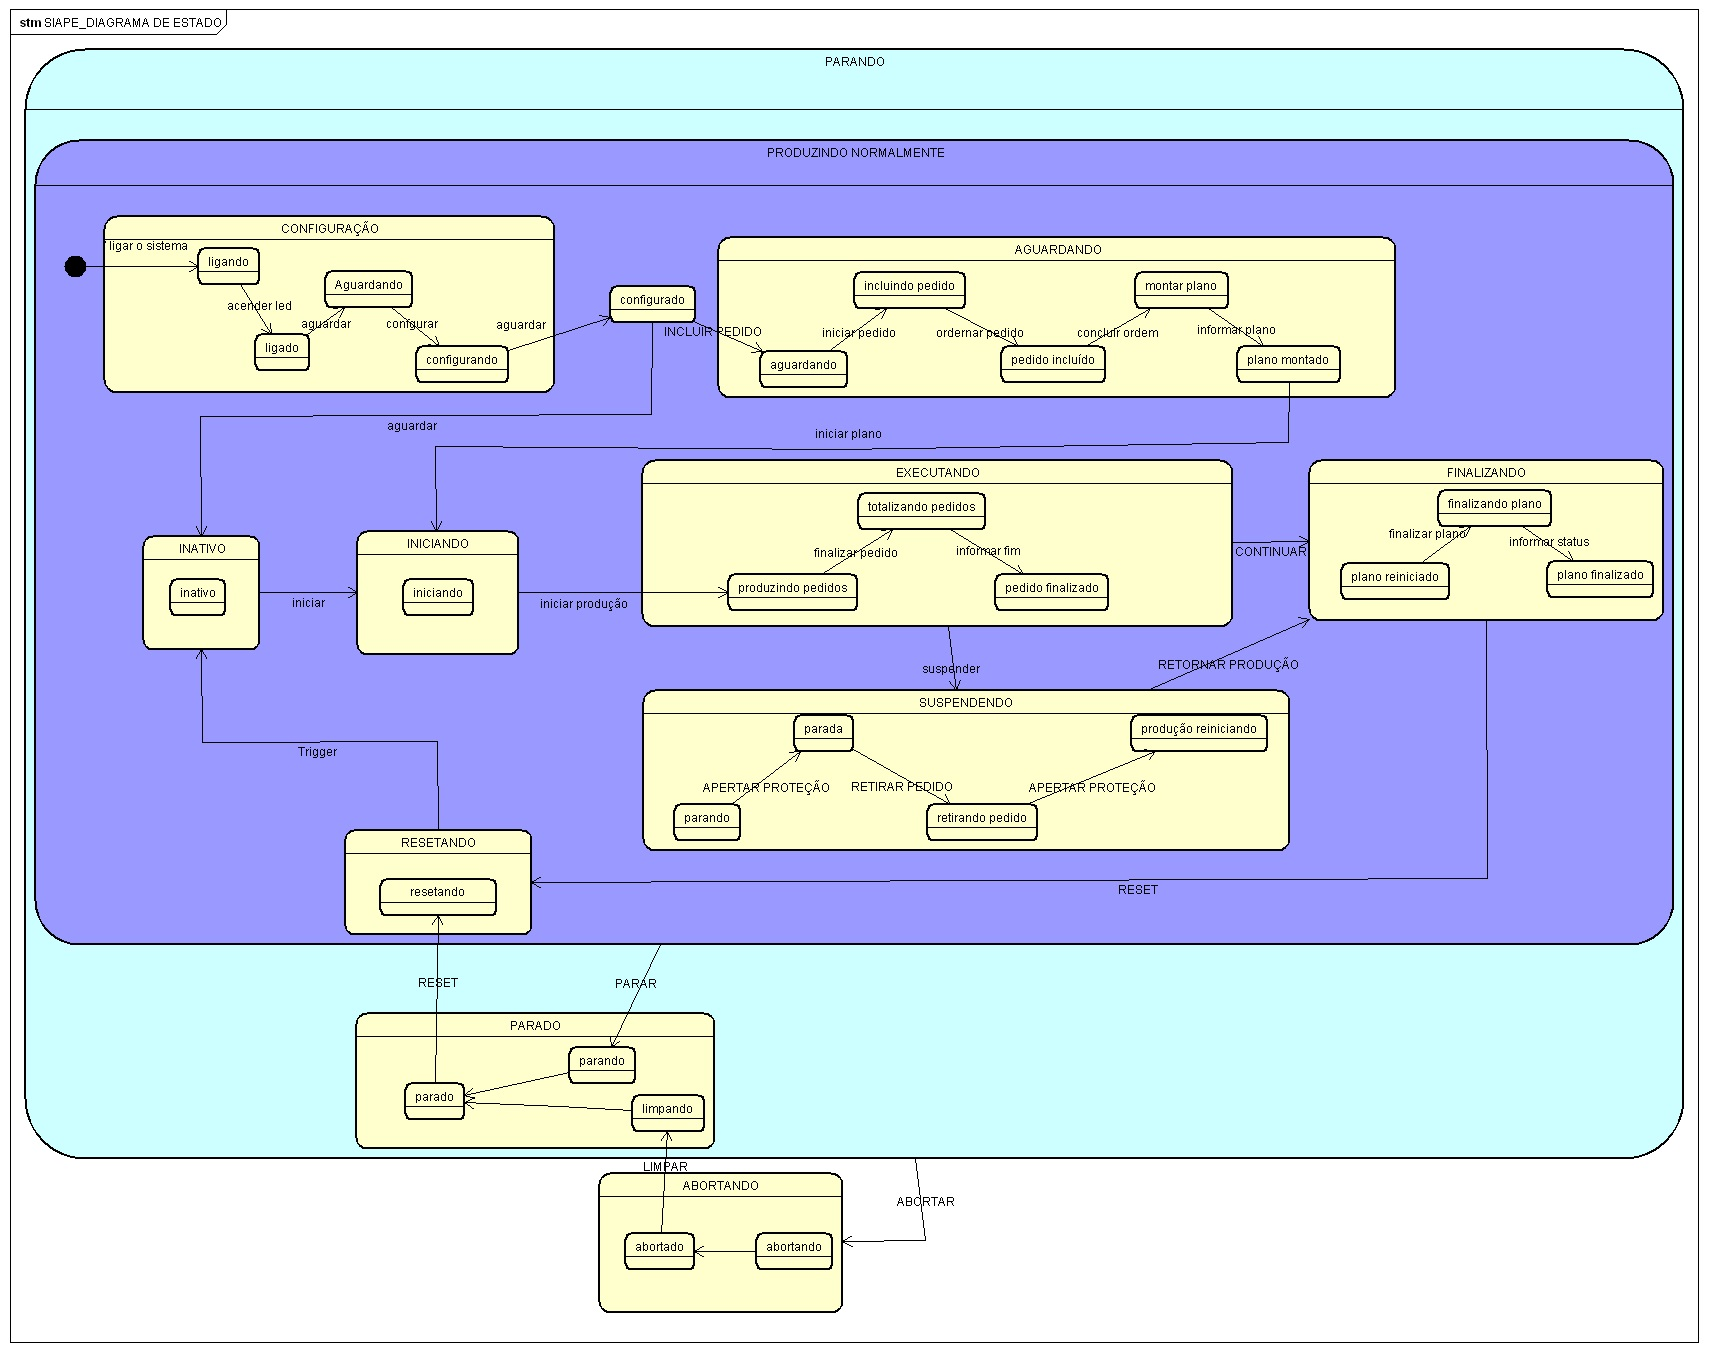
\includegraphics[width=26cm, height=16cm]{F79_SIAPE_DIAGRAMA_ESTADO.jpg} 
		\caption{SIAPE: Diagrama de estados}
		\label{F79}
	\end{figure}
\end{landscape}
 		 
 	A seguir são realizadas breves descrições dos processos de modelagem e simulação para facilitar o entendimento do processo:\par 
  
 	\begin{description}
 	\item [1. Esteira -] 	
 	 O Módulo Esteira foi modelado seguindo as Leis de \textit{Kirchoff} para a parte elétrica, e as Leis de \textit{Hooke} para a parte mecânica. Após a modelagem eletro-mecânica definiu-se a forma da esteira e realizou-se a montagem experimental das partes e  mecânica. A simulação foi realizada e os resultados permitiram a inclusão dos requisitos refinados como especificações técnicas relativas às partes elétricas e mecânicas do módulo. A Figura \ref{F69} ilustra esse processo.
 	 \begin{figure}[!h]
 	 	\centering
 	 	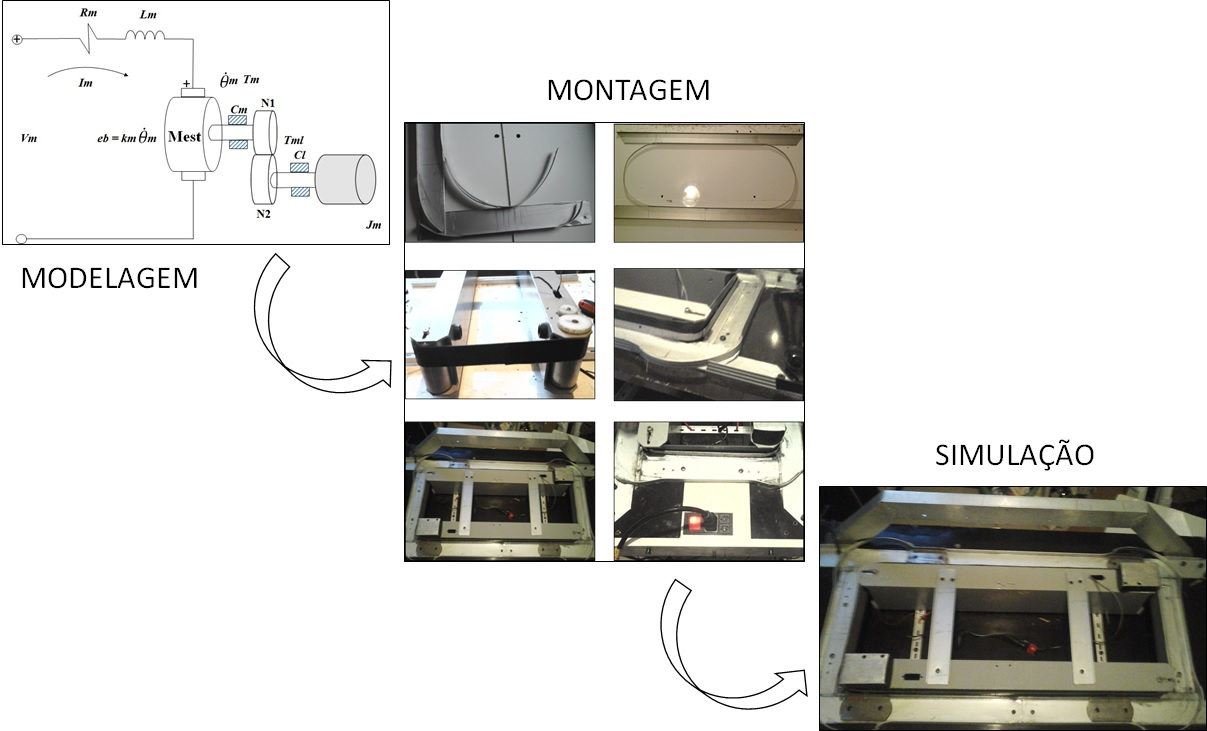
\includegraphics[width=13cm, height=6cm]{F69_SIAPE_ESTEIRA.jpg} 
 	 	\caption{Esteira:  Da modelagem à simulação}
 	 	\label{F69}
 	 \end{figure}
 	 
 	\item[2. Carimbador -]  
 	Da mesma forma que a esteira,  o Módulo Carimbador foi modelado seguindo as Leis de \textit{Kirchoff} para a parte elétrica, e as Leis de \textit{Hooke} para a parte mecânica. Após a modelagem eletro-mecânica definiu-se a forma de um módulo para que fosse realizada a montagem experimental de um módulo. A simulação foi realizada e os resultados permitiram a inclusão dos requisitos refinados como especificações técnicas relativas às partes elétricas e mecânicas do módulo. A Figura \ref{F70} ilustra esse processo.	
 	 \begin{figure}[!h]
 	 	\centering
 	 	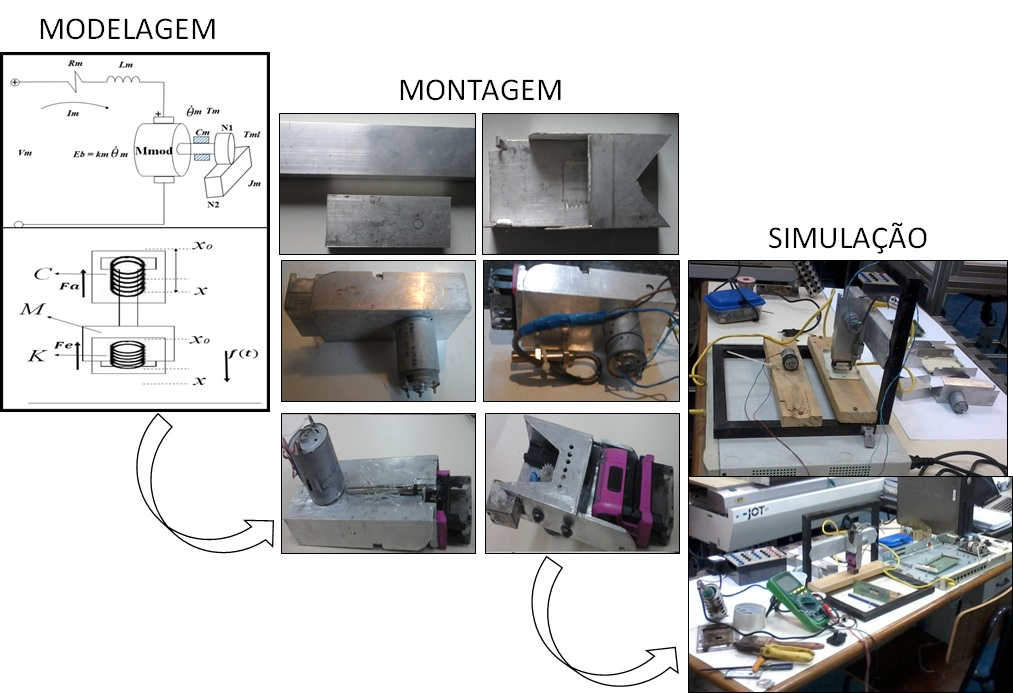
\includegraphics[width=13cm, height=6cm]{F70_SIAPE_MODULO.jpg} 
 	 	\caption{Carimbador: Da modelagem à simulação}
 	 	\label{F70}
 	 \end{figure}
 	 
 	  \item[3. Agente AcHw - ] 
 	  A classe Acesso Hardware foi modelada com a principal função de identificar os módulos que estão presentes no  sistema e disponibilizar para o agente YPA. A Figura \ref{F71} ilustra a criação do código da classe e posterior simulação que evidenciou o seu funcionamento e aprovou sua inclusão como especificação técnica de software.  
 	  \begin{figure}[h]
 	  	\centering
 	  	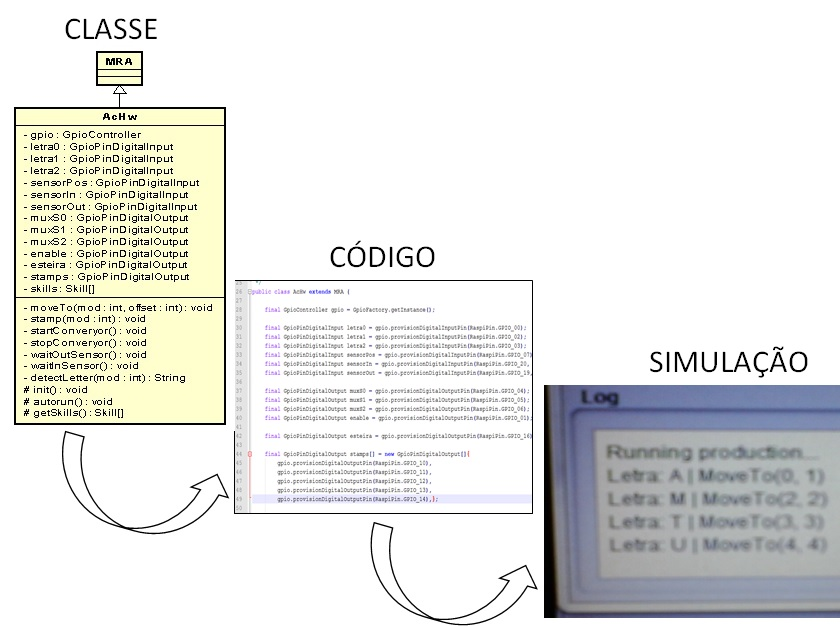
\includegraphics[width=13cm, height=6cm]{F71_SIAPE_CLASSE_ACHW.jpg} 
 	  	\caption{Classe AcHw}
 	  	\label{F71}
 	  \end{figure}
 	  
 	  \item[4. Agente YPA - ]
 	    A classe YPA foi modelada com a principal função de registrar os módulos que estão presentes no  sistema e disponibilizar para o agente Order. A Figura \ref{F72} ilustra a criação do código da classe e posterior simulação que evidenciou o seu funcionamento e aprovou sua inclusão como especificação técnica de software.  
 	  	
 	  \begin{figure}[!h]
 	  	\centering
 	  	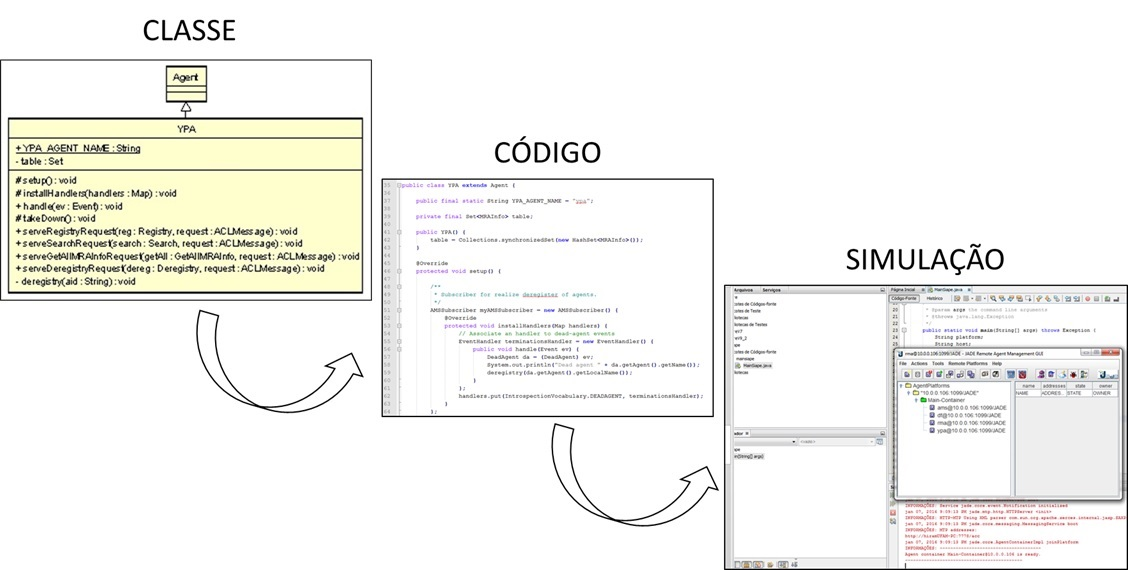
\includegraphics[width=13cm, height=6cm]{F72_SIAPE_CLASSE_YPA.jpg} 
 	  	\caption{Modelagem Classe YPA}
 	  	\label{F72}
 	  \end{figure}
 	  
 	  \item[5. Agente Order - ]  
 	    A classe Order foi modelada com a principal função de montar o plano com os módulos que estão presentes no  sistema e enviar para o agente Anagrama realizar a produção. A Figura \ref{F73} ilustra a criação do diagrama UML e o código da classe e posterior simulação que evidenciou o seu funcionamento e aprovou sua inclusão como especificação técnica de software.  
 	  	
 	  \begin{figure}[!h]
 	  	\centering
 	  	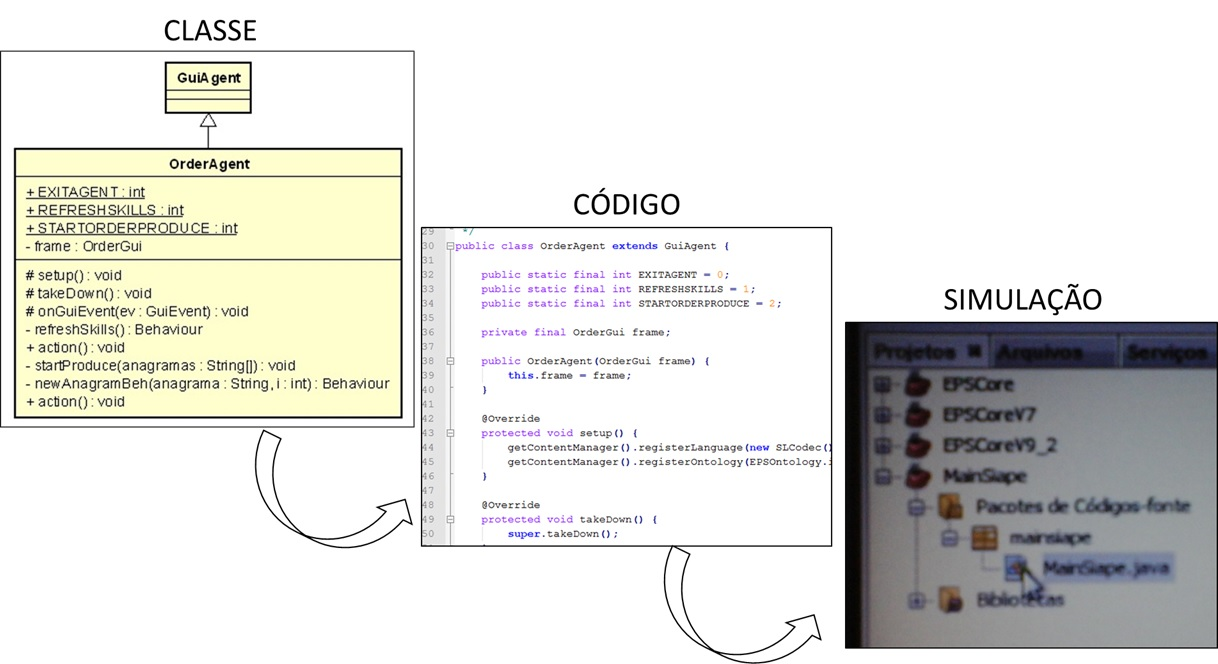
\includegraphics[width=13cm, height=6cm]{F73_SIAPE_CLASSE_ORDER.jpg} 
 	  	\caption{Modelagem classe Order}
 	  	\label{F73}
 	  \end{figure}
 	   	  
 	 \item[6. Agente Anagrama - ] 
 	  A classe Anagrama foi modelada com a principal função de realizar a produção do plano de produção com os módulos presentes no  sistema. A Figura \ref{F74} ilustra a criação do código da classe e posterior simulação que evidenciou o seu funcionamento e aprovou sua inclusão como especificação técnica de software.  
 	 	
 	  \begin{figure}[!h]
 	  	\centering
 	  	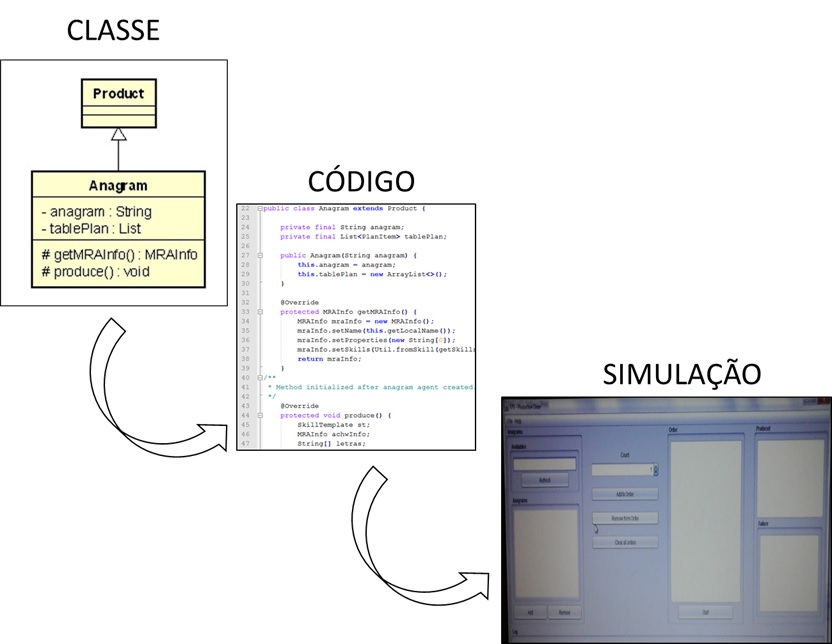
\includegraphics[width=13cm, height=6cm]{F74_SIAPE_CLASSE_ANAGRAMA.jpg} 
 	  	\caption{Modelagem classe Anagrama}
 	  	\label{F74}
 	  \end{figure}
 	  
 	  	  	   	  
 	  \item[7. Protocolo FIPA - ] 
 	  O principal objetivo do Protocolo FIPA é a comunicação entre os agentes do sistema. A Figura \ref{F94} ilustra a criação da classe OrderAgent, um trecho do código e a troca de mensagens capturada pelo agente Sniffer do Framework Jade.  
 	  
 	  
 	   \begin{figure}[!h]
 	   	\centering
 	   	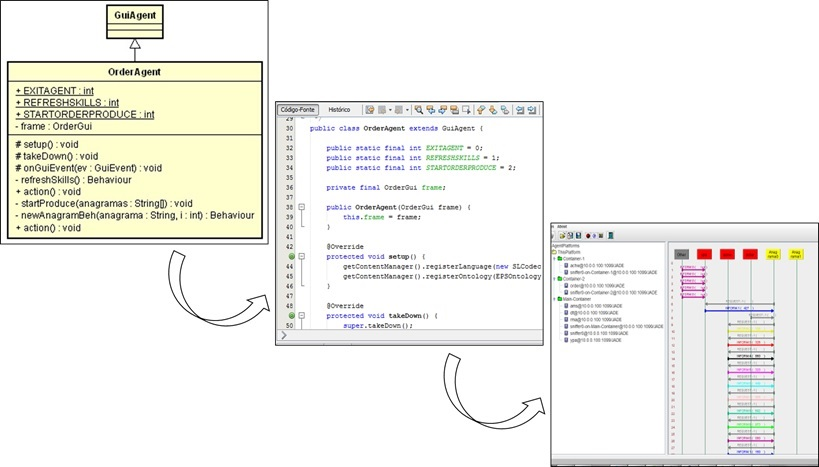
\includegraphics[width=13cm, height=6cm]{F94_SIAPE_FIPA.jpg} 
 	   	\caption{Modelagem Mensagens FIPA}
 	   	\label{F94}
 	   \end{figure}	  
 	\end{description}
 	
 	
 Nesta etapa os requisitos refinados do sistema em forma de problema global (RQRg), na forma regional  (RQRr) e local (RQRl) são modelados e simulados (SimM, SimE, SimS e SimC) até que estes possam ser garantidos como Especificações Técnicas (Et) de cada problema local, a saber: Especificação Técnica Mecânica (EtM), Especificação Técnica Elétrica (EtE), Especificação Técnica de Software (EtS) e Especificação Técnica de Comunicação (EtC). 
 
A Figura \ref{F95} ilustra esse processo para a parte de hardware. Os módulos selecionados com características de hardware foram modelados e rotulados conforme a sua funcionalidade dentro sistema. Esses módulos foram simulados e seus status  foram elevados à categoria de especificações. O significado de cada sigla é explicado a seguir e suas descrições serão realizadas na próxima etapa. 
	\begin{description}
	\begin{figure}[!h]
	\centering
	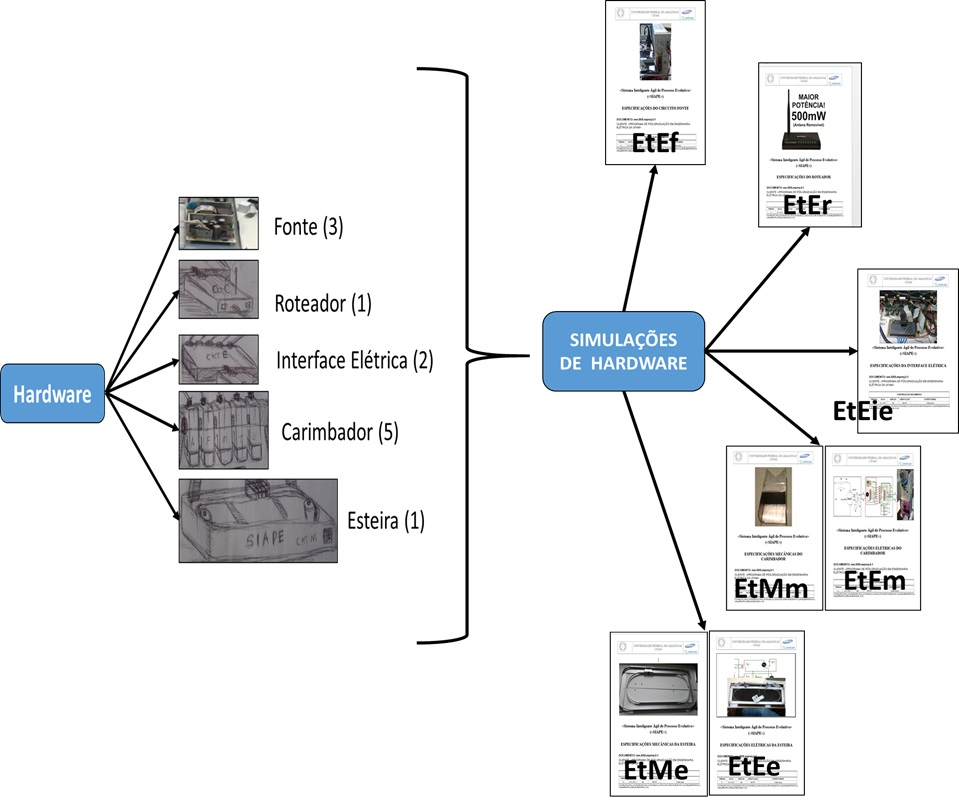
\includegraphics[width=13cm, height=6cm]{F95_SIAPE_SIM_HW.jpg} 
	\caption{Simulação de Hardware}
	\label{F95}
	\end{figure}  
		
		\item[1. EtMm] - Especificação técnica mecânica do módulo;
		\item[2. EtMe] - Especificação técnica mecânica da esteira;
		\item[3. EtEe] - Especificação técnica elétrica da esteira;
		\item[4. EtEf] - Especificação técnica elétrica das fontes;
		\item[5. EtEr] - Especificação técnica elétrica do roteador;
		\item[6. EtEie] - Especificação elétrica da interface elétrica; 
		\item[7. EtEm] - Especificação elétrica do módulo;
		\item[8. EtSis] - Especificação técnica da interface de software.
		
		\end{description}	
		
A Figura \ref{F96} ilustra esse processo para a parte de software. Os módulos selecionados com características de software foram modelados e rotulados conforme a sua funcionalidade dentro do sistema. Esses módulos foram simulados e seus status  foram elevados à categoria de especificações. O significado de cada sigla é explicado a seguir e suas descrições serão realizadas na próxima etapa. 		
		\begin{description}	
	
		 \begin{figure}[!h]
		 	\centering
		 	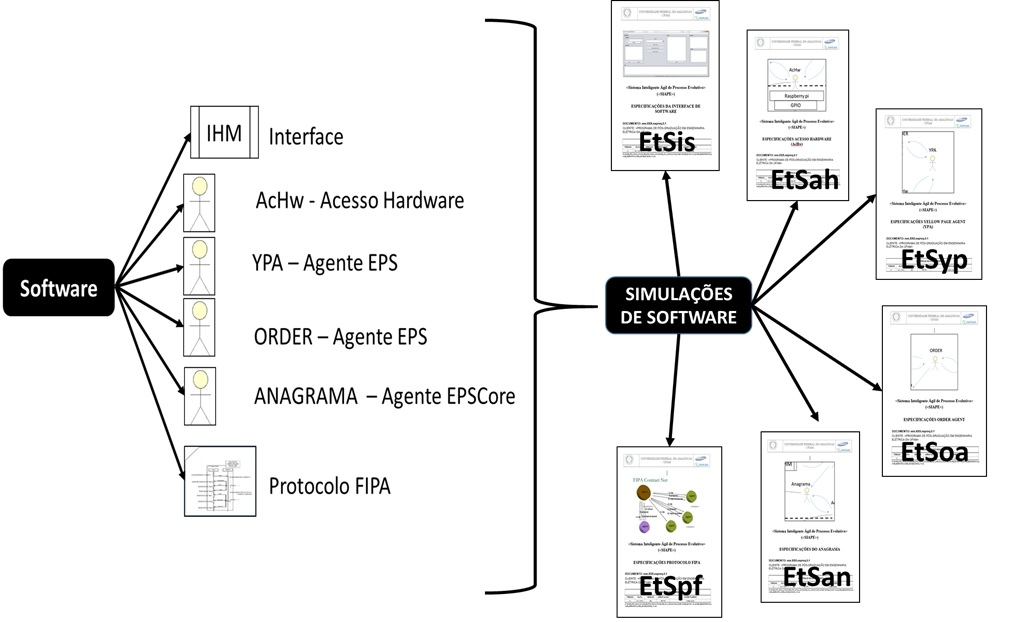
\includegraphics[width=13cm, height=6cm]{F96_SIAPE_SIM_SW.jpg} 
		 	\caption{Simulação de  Software                                                                                                                                                                                                                                                                                                                                                                                                                                                                                                                                                                                                                                                                                                                                                                                                                                                                                                                                                                                                                                                                                                                                                                                                                                                                                                                                     }
		 	\label{F96}
		 \end{figure}

		\item[9. EtSah] - Especificação técnica de software do agente acesso hardware;
		\item[10. EtSyp] - Especificação técnica de software do \textit{Yellow Page Agent(YPA)};
		\item[11. EtSao]  Especificação técnica de software o agente Order;
		\item[12. EtSan] - Especificação técnica de software do agente Anagrama;
		\item[13. EtSpf] - Especificação técnica de software dos protocolos FIPA.	
	\end{description}


 Estas especificações técnicas evidenciam o terceiro marco e servirão de base para do Projeto do Sistema. Na próxima etapa essas especificações serão organizadas no formato de projeto do sistema a ser implementado. 
 
 
  
 %=================================== ETAPA 4 ==================================
 \newpage
 %+++++++++++++++++++++++++++++++++++++++++++++++++++++++
\subsection{ETAPA 4 - PROJETOS}

\begin{description}

\begin{table}[htbp]
	\centering
	\caption{Tabela da etapa 4 - Projetos}
	%=================================================================================================
	\begin{tabular}{|l| p{13.5cm}| c| c| } \hline
		%================================================================================================
		\textbf{Item} 	    & \textbf{Descrição} 
		\\ \hline
		%================================================================================================
		\textbf{1. Objetivos}	   &  
		Integrar as especificações técnicas do sistema no documento de projeto.
		
		\\ \hline
		%================================================================================================
		\textbf{2. Entradas}	  &		
		EtM - Especificações técnicas da parte mecânica, EtE - Especificações técnicas da parte elétrica, EtS - Especificações técnicas da parte de software e EtC - Especificações técnicas da parte de comunicação. \par  	
		
		\\ \hline	
		%================================================================================================	
		\textbf{3. Processo}     &
		As especificações técnicas de hardware e software são organizadas no documento denominado de projeto de sistema.
		
		\\ \hline
		%================================================================================================
		\textbf{4. Saídas}		& 
		\textbf{Documento de Projeto de Sistema contendo as especificações técnicas de hardware, software e requisitos não-funcionais.}  
		
		\\ \hline
		%================================================================================================		
		\textbf{5. Registros}   & 	
		Casos de uso, resultados das simulações, requisitos refinado, requisitos iniciais, requisitos funcionais e não-funcionais. 
		\\ \hline
		%================================================================================================
	\end{tabular}
	\label{T6}\par
	%	Fonte: Hiram Amaral
\end{table}
\item[Descrição textual e visual da etapa] - Para integrar as especificações técnicas - resultado das simulações da Etapa 3 - ao documento de projeto, essas são verificadas por meio dos diagramas de sequência, atividade e estado, pois esses diagramas são partes integrantes do projeto e fazem parte do projeto de classes do sistema. Definidos esses diagramas, eles são consolidados no documento do sistema. \par 		   
As especificações técnicas das partes mecânica, elétrica, de software e de comunicação que servirão de base para a definição dos diagramas a serem desenvolvidos são submetidos ao processo que as transformarão em diagramas de sequência, de atividades e de estado. O resultado é inserido no documento de projeto juntamente com as especificações técnicas de cada parte do sistema. \par 		
O resultado é evidenciado pelo documento de projeto de sistema que serve como evidência da entrega do quarto marco. 


\end{description}


		  \begin{figure}[!h]
		  	\centering
		  	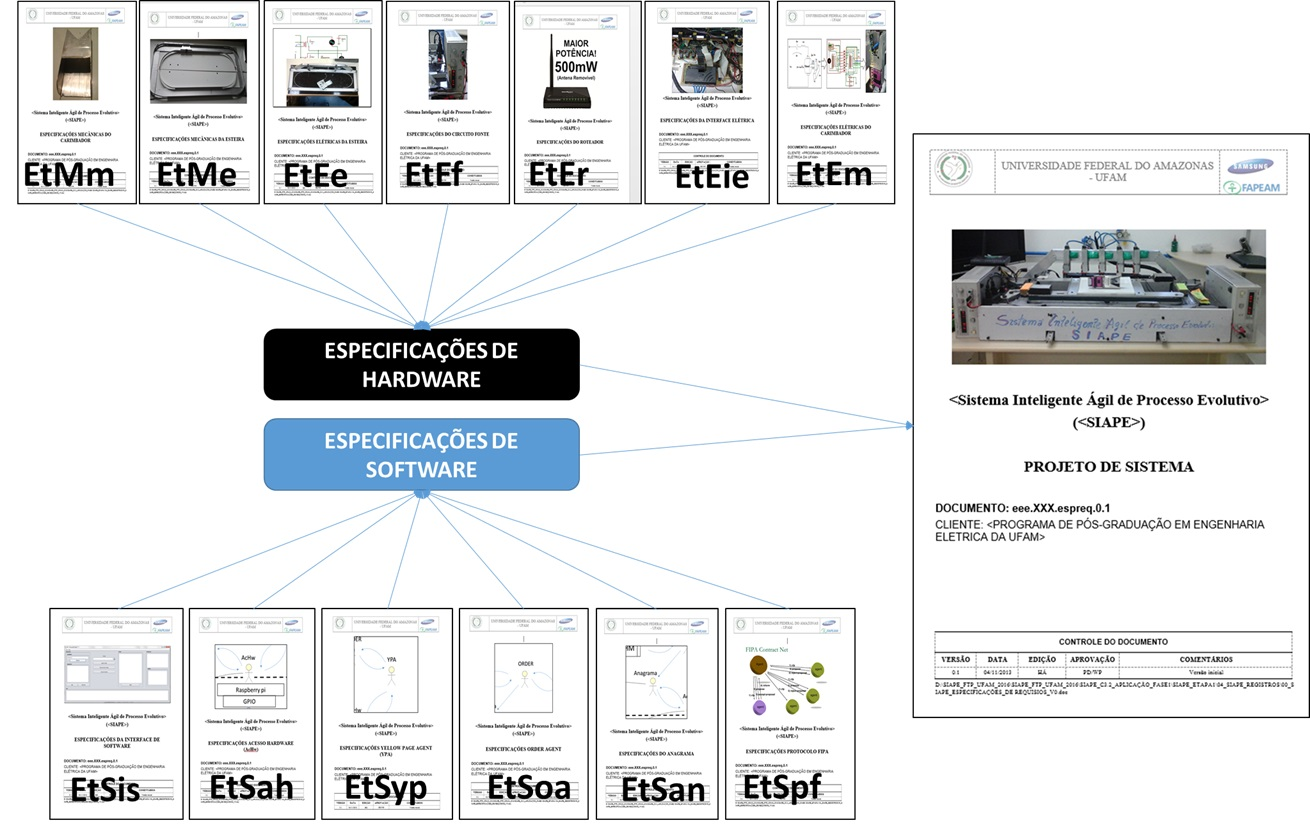
\includegraphics[width=16cm, height=10cm]{F80_SIAPE_PROJETO_SISTEMA.jpg} 
		  	\caption{Projeto de Sistema}
		  	\label{F80}
		  \end{figure}
		  
A Figura \ref{F80} ilustra a consolidação das especificações de hardware e software no documento do Projeto de Sistema. As descrições das especificações são relacionadas a seguir:
	 		\begin{description}
	 			\item[1. EtMm] - Especificação técnica mecânica define as medidas que deverão ser realizadas no material especificado para transformá-lo no protótipo mecânico do módulo;
	 			\item[2. EtMe] - Especificação técnica mecânica da esteira de define a forma que deverá ser desenvolvida para que o palete trafegue sem interferências;
	 			\item[3. EtEe] - Especificação elétrica da esteira define a alimentação do motor em valores de tensão e corrente que não devem ultrapassar os valores definidos como restrições para o projeto;
	 			\item[4. EtEf] - Especificação técnica elétrica das fontes especifica os valores de tensão e corrente para todos todo os módulos do sistema, e que atendem às restrições;
	 			\item[5. EtEr] - Especificação elétrica do roteador descreve os dados técnicos do roteador que serão utilizados para conectar os dispositivo do SIAPE;
	 			\item[6. EtEie] -  Especificação elétrica da interface elétrica define todos os componentes e circuitos elétricos que deverão ser implementados no sistema;
	 			\item[7. EtEm] - Especificação elétrica do módulo define os circuitos elétricos e que deverão ser implementados;
	 			\item[8. EtSis] - Especificação técnica de software da interface de software do sistema descreve os campos que devem ser implementados no sistema.
	 			\item[9. EtSah] - Especificação técnica de software descreve as características e habilidades do agente de acesso hardware;
	 			\item[10. EtSyp] - Especificação técnica de software descreve as características e habilidades do agente de Yellow Page Agent (YPA);
	 			\item[11. EtSao] - Especificação técnica de software descreve as características e habilidades do agente Order;
	 			\item[12. EtSan] - Especificação técnica de software descreve as características e habilidades do agente Anagrama;
	 			\item[13. EtSpf] - Especificação técnica de software descreve todos os protocolos utilizados no SIAPE. 		
	 		\end{description}

O Projeto de Sistema evidencia o quarto marco e contém as especificações que expressam o resultado de estudos que iniciaram com as necessidades do cliente, os referenciais internos e externos. Esses foram transformados em requisitos refinados, modelados e simulados para que as especificações pudessem ser garantidas como tal. Na Etapa 5 o Projeto de Sistema é implementado.

%=================================== ETAPA 5 ==================================

\clearpage
%+++++++++++++++++++++++++++++++++++++++++++++++++++++++
\subsection{ETAPA 5 - IMPLEMENTAÇÕES}

\begin{table}[htbp]
	\centering
	\caption{Tabela da etapa 5 - Implementações}
	%=================================================================================================
	\begin{tabular}{|l| p{13.5cm}| c| c| } \hline
		%================================================================================================
		\textbf{Item} 	    & \textbf{Descrição} 
		\\ \hline
		%================================================================================================
		\textbf{1.Objetivos}	   &  
		Implementar os projetos definidos na Etapa 4.
		\\ \hline
		%================================================================================================
		\textbf{2.Entradas}	  &		
		
		Projeto de hardware contendo os módulos mecânicos e elétricos.\par  	
		Projeto de software contendo os módulos de software e de comunicação. 
		\\ \hline	
		%================================================================================================	
		\textbf{3.Processo}     &
		Os projetos são implementados e transformados em protótipos das partes do sistema.
		\\ \hline
		%================================================================================================
		\textbf{4.Saídas}		& 
		Protótipo elétrico, protótipo mecânico, códigos do software e de comunicação.
		\\ \hline
		%================================================================================================		
		\textbf{5.Registros}   & 	
		Diagramas de classe, diagrama de sequência, diagrama de atividades, diagrama de estado, esquema elétrico e especificações técnicas.
		\\ \hline
		%================================================================================================
	\end{tabular}
	\label{T7}\par
	%	Fonte: Hiram Amaral
\end{table}

	\begin{description}
		
		\item[Descrição textual e visual da etapa] - A partir das especificações técnicas são desenvolvidos circuitos que atendam às especificações. Desses circuitos são originados os esquemas elétricos, as placas de circuito impresso (PCI) e são acoplados aos seus respectivos módulos. \par 
		
		
		\item[1. EtMm] - A especificação técnica mecânica define as medidas que deverão ser realizadas no material especificado para transformá-lo no protótipo mecânico do módulo;\par 
		
		  \begin{figure}[!h]
		  	\centering
		  	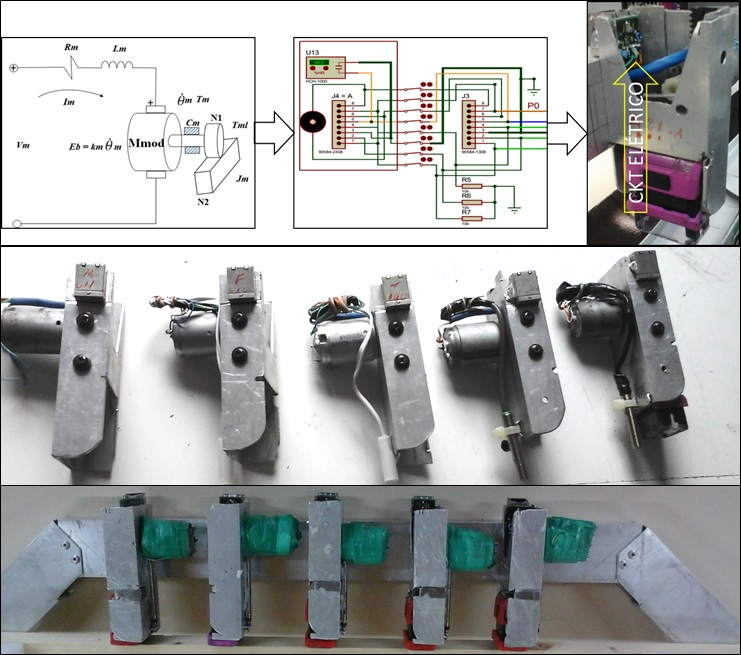
\includegraphics[width=13cm, height=9cm]{F81_SIAPE_MODULOS_LETRAS.jpg} 
		  	\caption{Evolução dos módulos: do circuito elétrico aos módulos}
		  	\label{F81}
		  \end{figure}
				
		\item[2. EtMe] - A especificação técnica mecânica da esteira de define a forma que deverá ser desenvolvida para que o palete trafegue sem interferências; \par 	
	
	 \begin{figure}[!h]
	 	\centering
	 	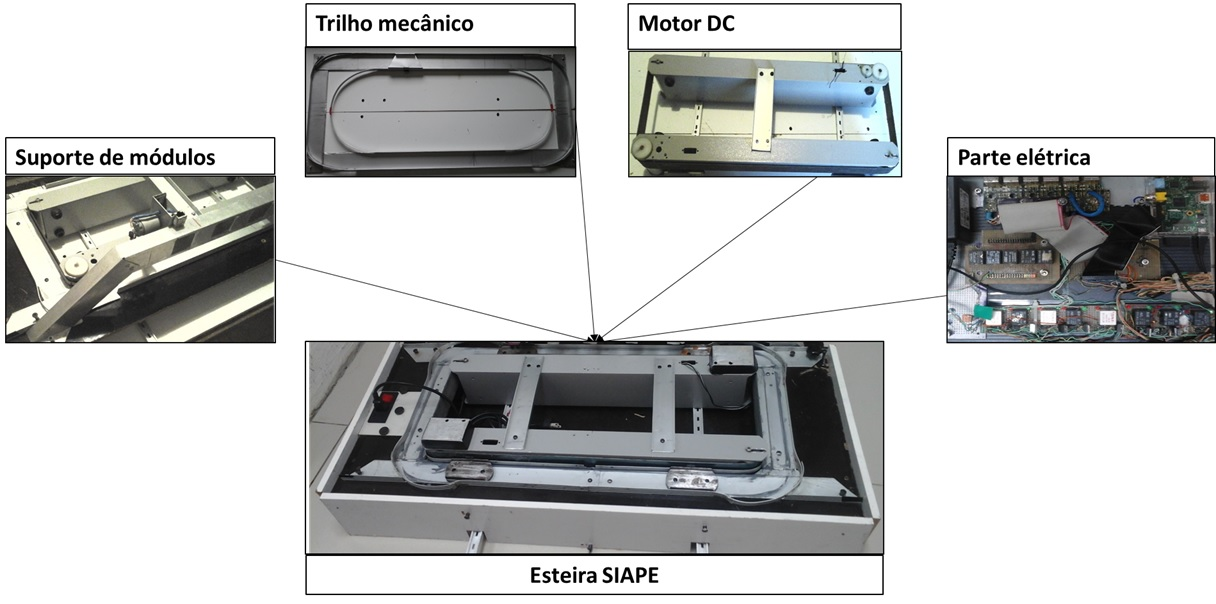
\includegraphics[width=13cm, height=5cm]{F82_SIAPE_ESTEIRA.jpg} 
	 	\caption{Evolução da esteira: do modelo ao protótipo}
	 	\label{F82}
	 \end{figure}
	
		\item[3. EtEe] - A especificação elétrica da esteira define a alimentação do motor em valores de tensão e corrente que não devem ultrapassar os valores definidos como restrições para o projeto;
		 
		 \begin{figure}[!h]
		 	\centering
		 	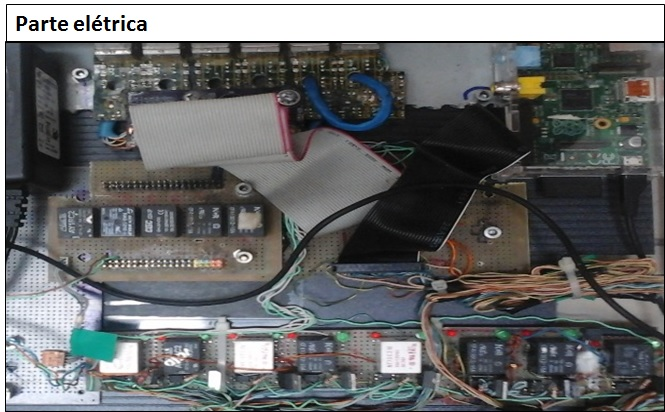
\includegraphics[width=12cm, height=5cm]{F83_SIAPE_PARTE_E.jpg} 
		 	\caption{SIAPE : Parte elétrica}
		 	\label{F83}
		 \end{figure}				
		
		\item[4. EtEf] - A especificação técnica elétrica das fontes especifica os valores de tensão e corrente para todos todo os módulos do sistema, e que atendem às restrições;
			 
			 \begin{figure}[!h]
			 	\centering
			 	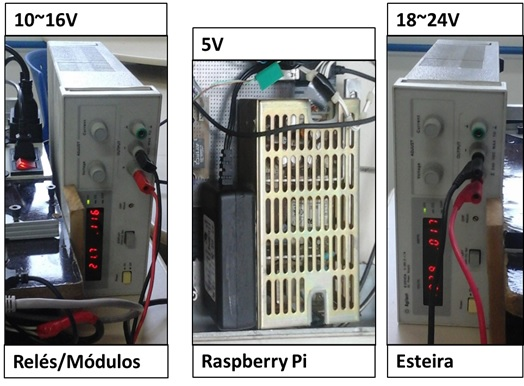
\includegraphics[width=11cm, height=5cm]{F84_SIAPE_FONTES.jpg} 
			 	\caption{SIAPE : Fontes}
			 	\label{F84}
			 \end{figure}
		
		\item[5. EtEr] - A especificação elétrica do roteador descreve os dados técnicos do roteador que serão utilizados para conectar os dispositivo do SIAPE;
		
		
			 \begin{figure}[!h]
			 	\centering
			 	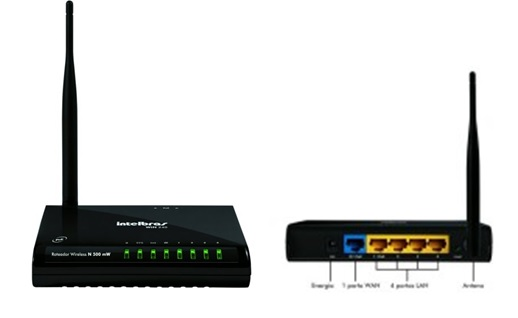
\includegraphics[width=11cm, height=4cm]{F85_SIAPE_ROTEADOR.jpg} 
			 	\caption{SIAPE : Roteador}
			 	\label{F85}
			 \end{figure}
		
		\item[6. EtEie] -  A especificação elétrica da interface elétrica define todos os componentes e circuitos elétricos que deverão ser implementados no sistema;
		
		
		 \begin{figure}[!h]
		 	\centering
		 	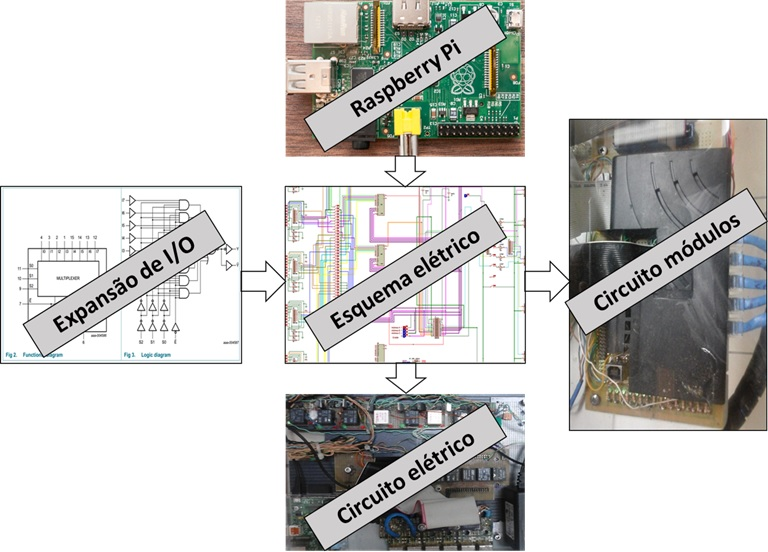
\includegraphics[width=10cm, height=5cm]{F86_SIAPE_INTERFACE_ELETRICA.jpg} 
		 	\caption{SIAPE : Interface elétrica}
		 	\label{F86}
		 \end{figure}
		
		\item[7. EtEm] - A especificação elétrica do módulo define os circuitos elétricos e que deverão ser implementados;
		
		 \begin{figure}[!h]
		 	\centering
		 	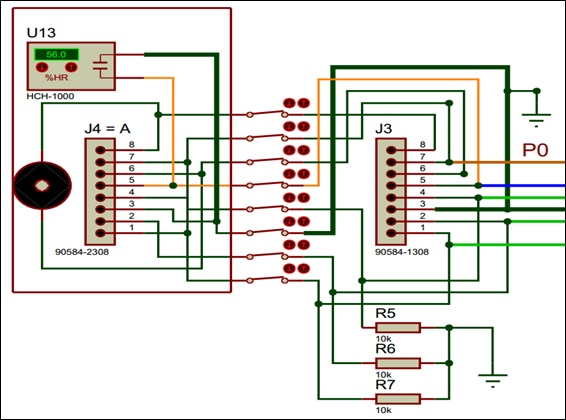
\includegraphics[width=8cm, height=5cm]{F87_SIAPE_ELETRICA_MOD.jpg} 
		 	\caption{SIAPE : Circuito elétrico módulo }
		 	\label{F87}
		 \end{figure}
		
		
		\item[8. EtSis] - A especificação técnica de software da interface de software do sistema descreve os campos que devem ser implementados no sistema.

		 \begin{figure}[!h]
		 	\centering
		 	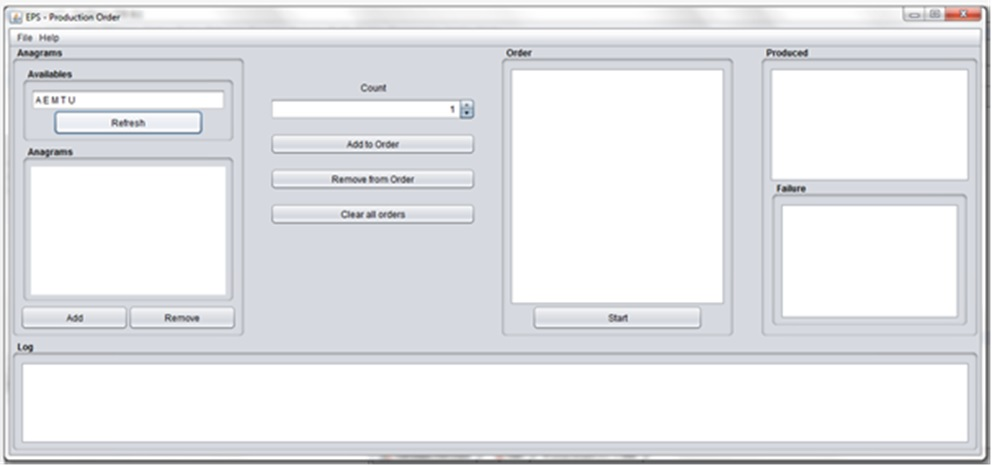
\includegraphics[width=14cm, height=7cm]{F88_SIAPE_INTERFACE.jpg} 
		 	\caption{SIAPE : Interface}
		    \label{F88}
		 \end{figure}

		\item[9. EtSah] - A especificação técnica de software descreve as características e habilidades do agente de acesso hardware;
			
		 \begin{figure}[!h]
		 	\centering
		 	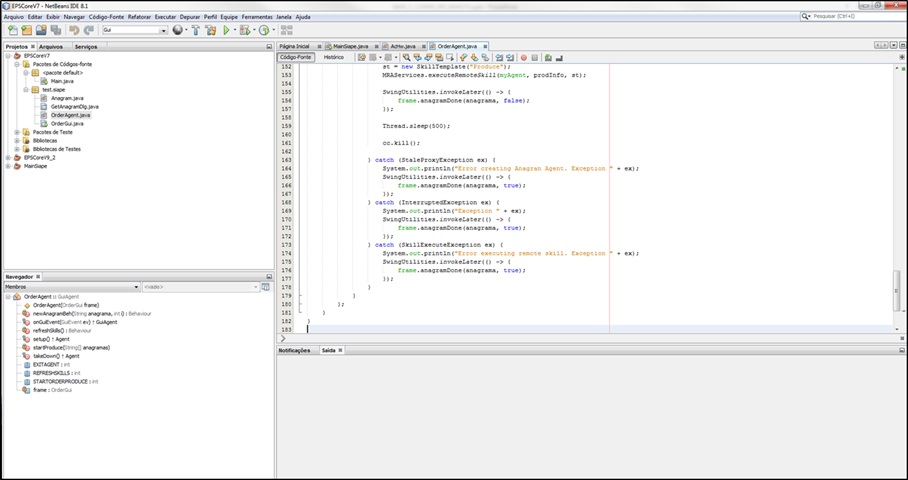
\includegraphics[width=14cm, height=7cm]{F89_SIAPE_ACHW.jpg} 
		 	\caption{SIAPE : Acesso Hardware}
		 	\label{F89}
		 \end{figure}
		
		\item[10. EtSyp] - A especificação técnica de software descreve as características e habilidades do agente de Yellow Page Agent(YPA);
		
		 \begin{figure}[!h]
		 	\centering
		 	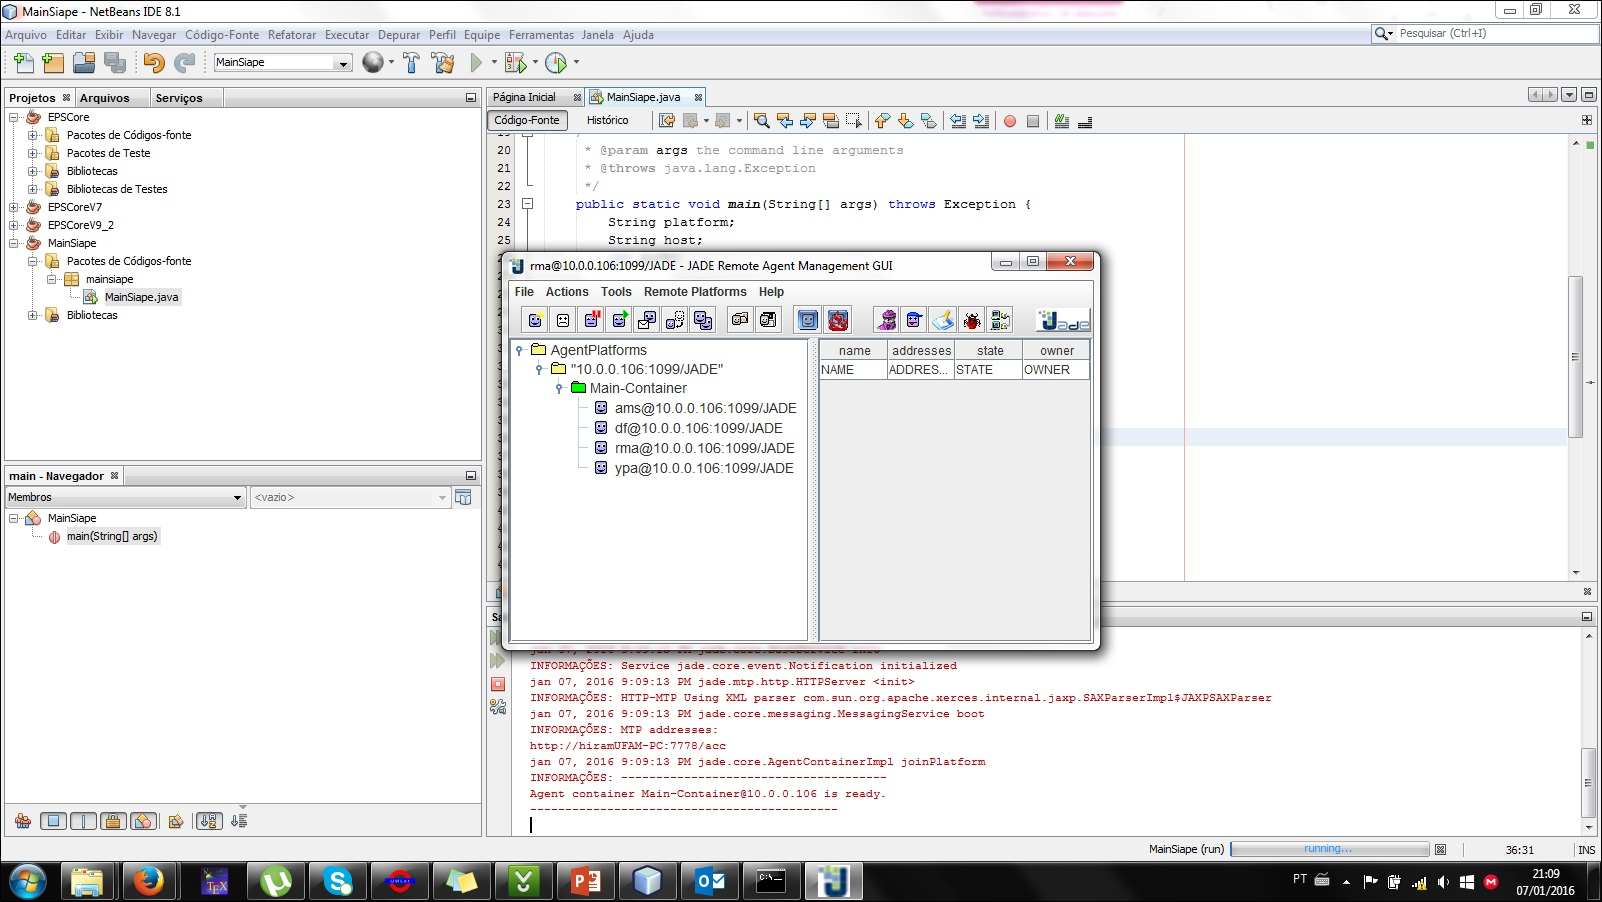
\includegraphics[width=14cm, height=7cm]{F90_SIAPE_YPA.jpg} 
		 	\caption{SIAPE: YPA}
		 	\label{F90}
		 \end{figure}	
				
		\item[11. EtSao] - A especificação técnica de software descreve as características e habilidades do agente Order;
				
		 \begin{figure}[!h]
		 	\centering
		 	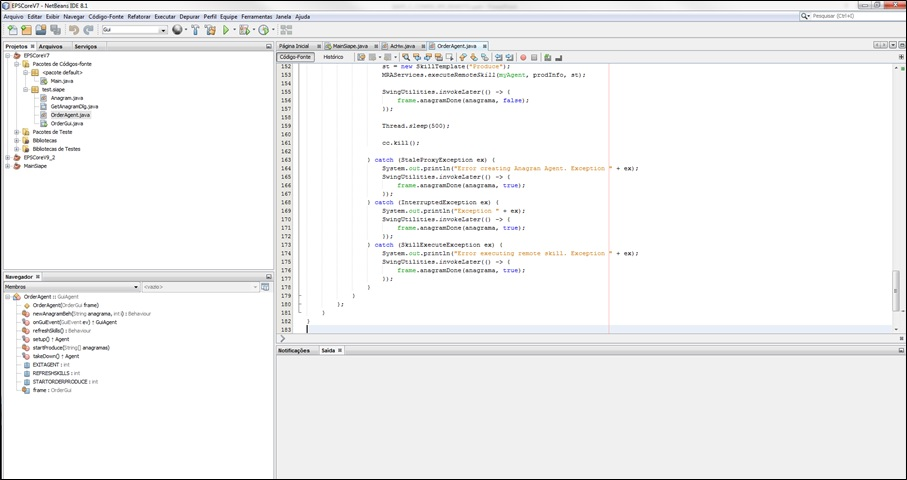
\includegraphics[width=14cm, height=7cm]{F91_SIAPE_ORDER.jpg} 
		 	\caption{SIAPE: ORDER}
		 	\label{F91}
		 \end{figure}			
		
		\item[12. EtSan] - A especificação técnica de software descreve as características e habilidades do agente Anagrama;
		
	 \begin{figure}[!h]
	 	\centering
	 	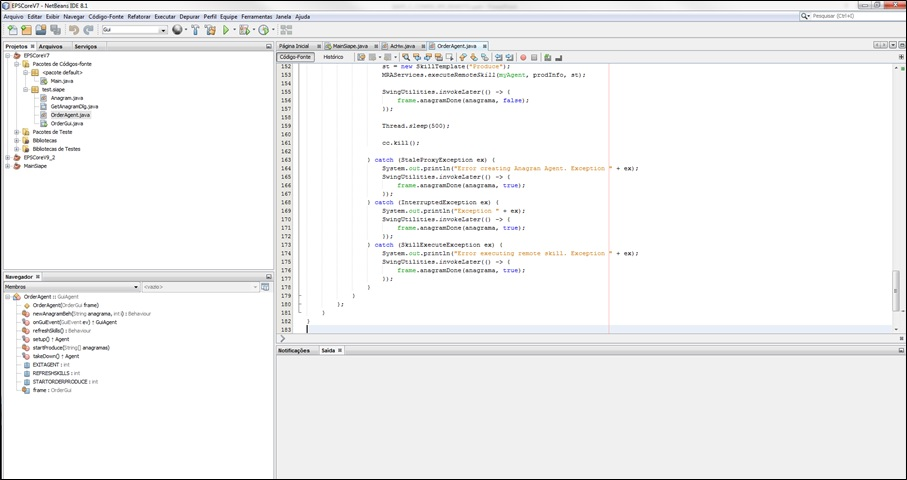
\includegraphics[width=14cm, height=7cm]{F91_SIAPE_ORDER.jpg} 
	 	\caption{SIAPE: ANAGRAMA}
	 	\label{F92}
	 \end{figure}			
		
		\item[13. EtSpf] - A especificação técnica de software descreve todos os protocolos utilizados no SIAPE.	
	\end{description}


Cada módulo é denominado com um nome de protótipo da parte específica do sistema. Estes módulos seguem para a Etapa 6 onde deverão ser testados contra as especificações técnicas e requisitos refinados.  

%=================================== ETAPA 6 ==================================

\clearpage
%+++++++++++++++++++++++++++++++++++++++++++++++++++++++
\subsection{ETAPA 6 - TESTES}

\begin{table}[htbp]
	\centering
	\caption{Tabela da etapa 6 - Testes}
	%=================================================================================================
	\begin{tabular}{|l| p{13.5cm}| c| c| } \hline
		%================================================================================================
		\textbf{Item} 	    & \textbf{Descrição} 
		\\ \hline
		%================================================================================================
		\textbf{1.Objetivos}	   &  
		Testar os protótipos implementados na Etapa 5.
		\\ \hline
		%================================================================================================
		\textbf{2.Entradas}	  &		
		Protótipo mecânico, protótipo elétrico, códigos do software, protocolos de comunicação FIPA. 
		\\ \hline	
		%================================================================================================	
		\textbf{3.Processo}     &
		Os protótipos funcionais implementados na Etapa 5 são submetidos aos testes especificados nos RQRs e Ets.
		\\ \hline
		%================================================================================================
		\textbf{4.Saídas}		& 
		Protótipo mecânico testado, protótipo elétrico testado, códigos do software testados, protocolos de comunicação FIPA testados.  	
		\\ \hline
		%================================================================================================		
		\textbf{5.Registros}   & 	
		RQRs, Ets, resultados dos testes.
		\\ \hline
		%================================================================================================
	\end{tabular}	
	\label{T8}\par
	%	Fonte: Hiram Amaral
\end{table}

\begin{description}
	
\item[Descrição textual e visual da etapa] - Os protótipos funcionais são submetidos aos testes especificados, individualmente, com o objetivo de testar sua funcionalidade contra os requisitos refinados e contra as especificações.\par 
Havendo a aprovação dos testes, os protótipos assumem o status de protótipos aprovados e preparados para serem integrados.

\end{description}

Na Figura \ref{F97} pode ser visualizado um resumo dos testes aplicados às partes ou ao todo durante a Etapa. As descrições encontram-se a seguir de acordo com a numeração:
	\begin{description}
		\item[ Número 1 ] - Este teste objetiva testar a funcionalidade do motor, o trajeto da esteira e a robustez do módulo mecânico da esteira. A alimentação de corrente é aplicada diretamente ao motor DC, neste caso variando a tensão entre os limites de 10V a 16V.  

	\begin{figure}[h]
		\centering
		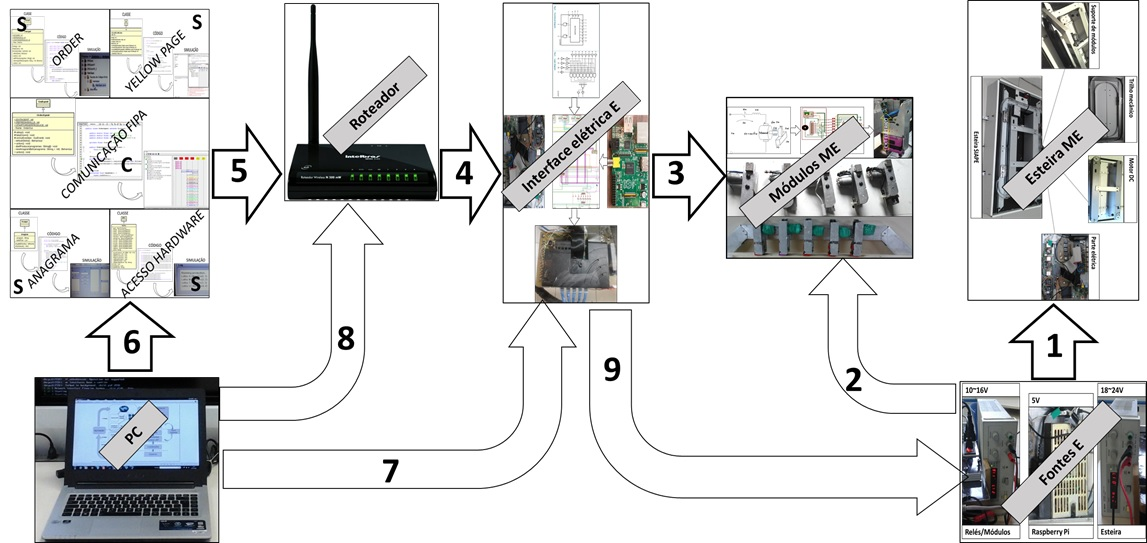
\includegraphics[width=16cm, height=7cm]{F97_SIAPE_TESTES.jpg} 
		\caption{Etapa de testes}
		\label{F97}
	\end{figure}

	\item[ Número 2 ] - Da mesma forma que foi aplicado à esteira, este teste objetiva testar a funcionalidade do motor, o trajeto do carimbo e a robustez do módulo mecânico das letras. A alimentação de corrente é aplicado diretamente ao motor DC, neste caso variando a tensão entre os limites de 16V a 24V;

	\item[ Número 3 ] - Este teste objetiva testar a funcionalidade do módulo eletro-mecânico através do comando do software.  Três maneiras podem ser utilizadas para realizar este teste: Utilizar os comando por meio do PC (Número 7) aplicados diretamente à interface elétrica, ou por meio dos números 6, 5, 4, e 3, ou ainda por meio dos números 8, 4 e 3. Percebe-se uma entidade MES é realizada;  
	
	\item[ Número 4 ] - O PC acessa a interface elétrica via roteador e manda os comandos para o módulo ME. Há que se perceber que, também neste caso, uma entidade MES é realizada;
	
	
	\item[ Número 5 ] - O PC acessa a interface elétrica via roteador e protocolo FIPA, e manda os comandos para o módulo ME. Há que se perceber que, neste caso, uma entidade MESC é realizada;	
	
	\item[ Número 6 ] - O PC acessa a interface elétrica via roteador e manda os comandos para o módulo ME. Idêntico ao teste número 6;
	
	\item[ Número 7 ] - O PC acessa a interface elétrica e manda os comandos para o módulo ME. Há que se perceber que, também neste caso, uma entidade MES é realizada;
	
	\item[ Número 8 ] - O PC acessa a interface elétrica via roteador e manda os comandos para o módulo ME. Há que se perceber que, também neste caso, uma entidade MESC é realizada;
	
	\item[ Número 9 ] - O PC acessa a interface elétrica e manda os comandos para o módulo ME da esteira. Há que se perceber que, também neste caso, uma entidade MES é realizada;


	\end{description}
	

	
A entrega dessas partes testadas evidencia a entrega do sexto marco. 
	
O resultado dessa etapa é o conjunto de partes individuais do sistema testadas e aprovadas para serem submetidas ao processo de integração na Etapa 7.\par





%=================================== ETAPA 7 ==================================
\clearpage
%+++++++++++++++++++++++++++++++++++++++++++++++++++++++
\subsection{ETAPA 7 - INTEGRAÇÃO MODULAR  E VALIDAÇÃO}

\begin{table}[htbp]
	\centering
	\caption{Tabela da etapa 7 - Integração modular e validação}
	%=================================================================================================
	\begin{tabular}{|l| p{13.5cm}| c| c| } \hline
		%================================================================================================
		\textbf{Item} 	    & \textbf{Descrição} 
		\\ \hline
		%================================================================================================
		\textbf{1.Objetivos}	   &  
		Integrar as partes aprovadas e e validar a integração.
		\\ \hline
		%================================================================================================
		\textbf{2.Entradas}	  &		
		 Protótipo mecânico testado,  protótipo elétrico testado,  códigos testado e protocolos testados.
		\\ \hline	
		%================================================================================================	
		\textbf{3.Processo}     &
		Protótipos testados são submetidos ao processo de integração e validação.
		\\ \hline
		%================================================================================================
		\textbf{4.Saídas}		& 
		Partes M, E, S e C integradas e validadas e preparadas para validação sistêmica. 
		\\ \hline
		%================================================================================================		
		\textbf{5.Registros}   & 
		Resultados dos testes e validações realizadas.
		\\ \hline
		%================================================================================================
	\end{tabular}
	\label{T9}\par
	%	Fonte: Hiram Amaral
\end{table}

\begin{description}
\item[Descrição textual e visual da etapa] - Os protótipos testados e aprovados são submetidos ao processo de integração de suas partes atômicas. \par 
Os protótipos M e E originam a parte integrada ME com suas características específicas, por exemplo, a parte mecânica é móvel e pode ser movida manualmente. A parte elétrica montada fornece as tensões para alimentar o motor. Ao se integrar essas partes, M e E produz-se uma entidade que pode ser alimentada eletricamente para que seja gerado um movimento eletro-mecânico. Ao se integrar a parte S à entidade ME, têm-se uma entidade ME automatizada. E finalmente, ao se integrar a parte C, ter-se-á uma entidade mecatrônica com suas características específicas.


\end{description}


\begin{figure}[h]
	\centering
	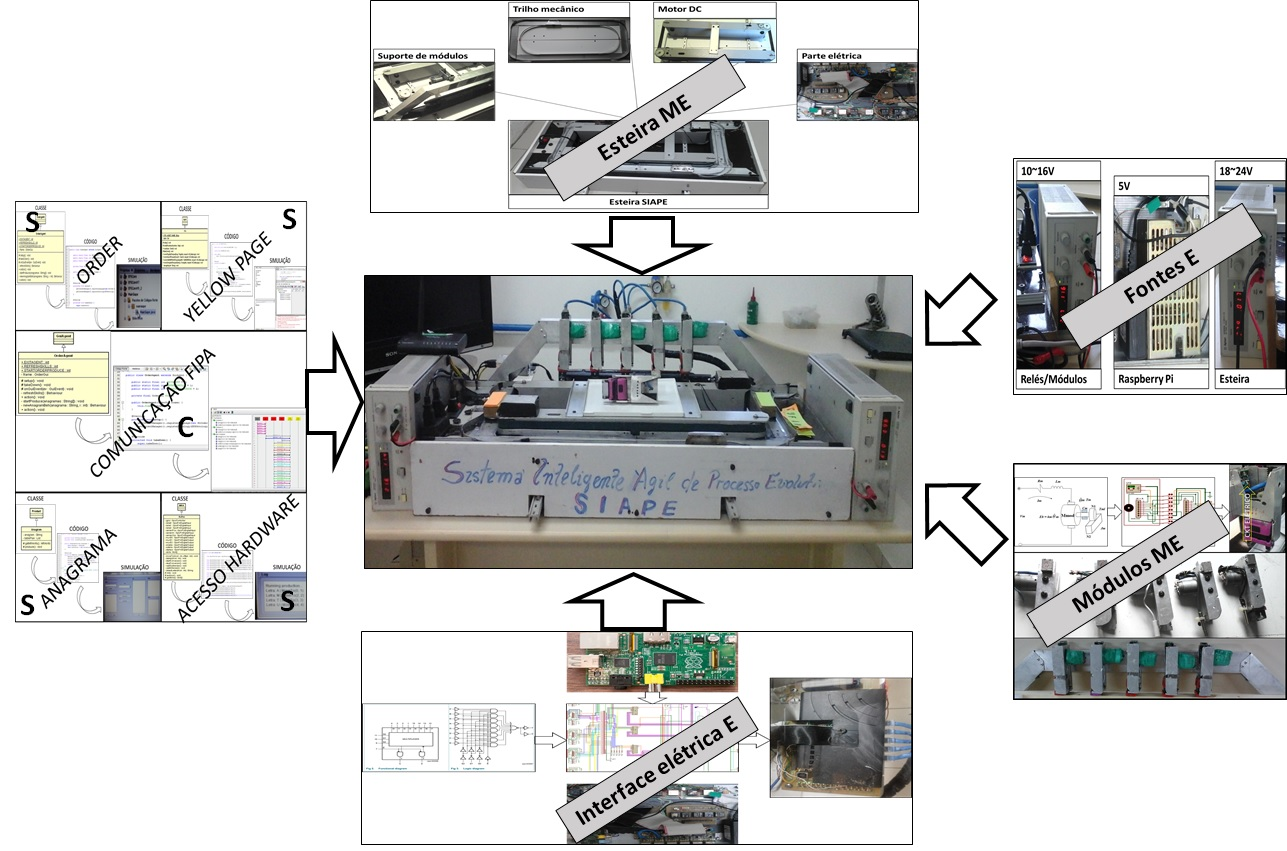
\includegraphics[width=16cm, height=7cm]{F98_SIAPE_INTEGRACAO_MODULAR.jpg} 
	\caption{Etapa de integração modular e validação}
	\label{F98}
\end{figure}


A Figura \ref{F98} ilustra a integração das partes Mecânicas, Eletrônicas, de Software e de Comunicação  e a realização do MESC. Essa integração modular é validada por meio da aplicação dos testes de números 1 a 9 da etapa anterior (Etapa 6). A diferença é que agora os módulos encontram-se integrados e todos os comandos são realizados no PC, e todos os dispositivos devem ser ligados à rede para que o protótipo MESC seja validado modularmente. Outra questão a ser observada é que os requisitos e especificações, neste estágio, são mais rígidos e devem ser tratados antes que o sistema siga para a integração validação sistêmica.    


Uma das validações é ilustrada na Figura \ref{F102} que valida tanto a parte de software quanto a parte de hardware na detecção de desconexão de módulos. Essa atividade é fundamental para a evidência do conceito \textit{plug and produce} durante a aplicação do estudo de caso no Capítulo 4. No detalhe tem-se do lado esquerdo, o sistema funcionando com todos os módulos, e a interface IDE retornando com todos as letras, no centro, tem-se desconexão do módulo. Do lado direito, em tempo real tem-se o sistema identificando a atividade e retornando a informação N.C. (não conectado).

 \begin{figure}[h]
 	\centering
 	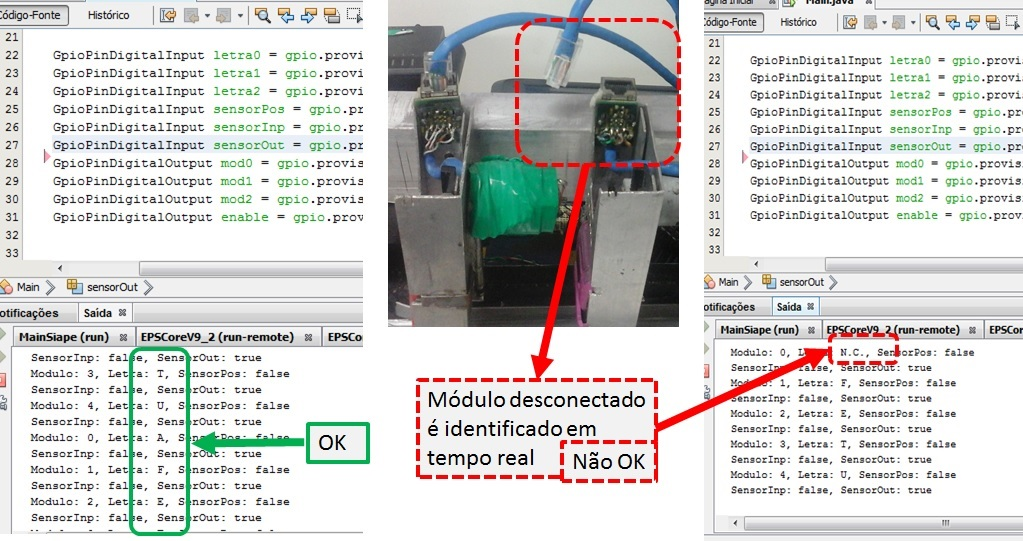
\includegraphics[width=16cm, height=7cm]{F102_SIAPE_DESCONEXAO.jpg} 
 	\caption{Detecção de desconexão de módulos}
 	\label{F102}
 \end{figure}


Além da rigidez na realização da validação modular, este também é o momento para organizar o material que será disponibilizado para o cliente e para os especialistas que irão ficar responsáveis pelo sistema, isto é, é o momento de finalizar os manuais técnico e de usuário. Esses manuais deverão ter suas eficácias postas à prova durante a Etapa de Comissionamento, isso para que potenciais erros possam ser identificados e evitem interferências no sistema quando da sua utilização pelos usuários do sistema.

A entrega do sistema validado modularmente evidencia o sétimo marco.



%=================================== ETAPA 8 ==================================
\clearpage

%+++++++++++++++++++++++++++++++++++++++++++++++++++++++
\subsection{ETAPA 8 - INTEGRAÇÃO E VALIDAÇÃO SISTÊMICA}

\begin{table}[htbp]
	\centering
	\caption{Tabela da etapa 8 - Integração e validação sistêmica}
	%=================================================================================================
	\begin{tabular}{|l| p{13.5cm}| c| c| } \hline
		%================================================================================================
		\textbf{Item} 	    & \textbf{Descrição} 
		\\ \hline
		%================================================================================================
		\textbf{1.Objetivos}	   &  
		Validar sistemicamente o protótipo modular do sistema.
		\\ \hline
		%================================================================================================
		\textbf{2.Entradas}	  &		
		Protótipo MESC integrado modularmente, requisitos iniciais co cliente, requisitos refinados e especificações técnicas. 
		\\ \hline	
		%================================================================================================	
		\textbf{3.Processo}     &
		O MESC é submetido ao processo de integração sistêmica contra as especificações e requisitos inciais.
		\\ \hline
		%================================================================================================
		\textbf{4.Saídas}		& 
		 SIAPE validado sistemicamente.
		\textbf{S1}  
		\\ \hline
		%================================================================================================		
		\textbf{5.Registros}   & 	
		Especificações técnicas, requisitos iniciais, requisitos refinados, manuais do sistema.
		\\ \hline
		%================================================================================================
	\end{tabular}
	\label{T10}\par
	%	Fonte: Hiram Amaral
\end{table}

\begin{description}
\item[Descrição textual e visual da etapa] - O protótipo MESC validado modularmente é submetido ao processo de validação sistêmica, aqui entendida como a validação que realiza um estudo de caso preparado pela equipe de desenvolvimento com o objetivo de evidenciar as funcionalidades  e performance do sistema e deverá ser reproduzida em parte ou no todo na próxima etapa com a presença do cliente e de seus especialistas. \par 
O estudo de caso deverá evidenciar tanto o atendimento das necessidades do cliente expressas no RQI quanto o atendimento aos requisitos refinados originados a partir dos RQI.\par 
\end{description}


A Figura \ref{F99} esboça a etapa de integração e validação sistêmica. Os documentos para esta etapa devem ser: 

\begin{description}
	\item[1 - DRQI] -  Documento de Requisitos iniciais o SIAPE
	\item[2 - DPS] - Documento de Projeto de Sistema
	\item[3 - MT] - Manual técnico do SIAPE
	\item[4 - MU] - Manual de usuário do SIAPE
\end{description}
	
Esses documentos são as referências que deverão ser consideradas para evidenciar o atendimento, ou não das necessidades do cliente, e nesta validação e estudo de caso deverá ser exaustivamente verificadas com o objetivo de comprovar a realização de todas as solicitações feitas pelo cliente e seus especialistas.
	
\begin{figure}[h]
	\centering
	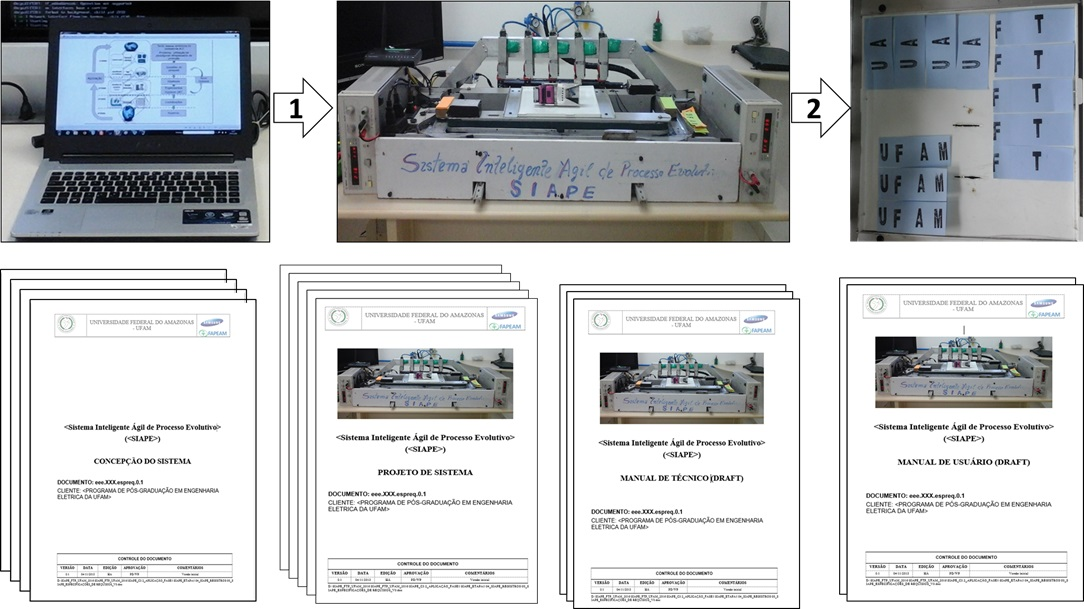
\includegraphics[width=16cm, height=9cm]{F99_SIAPE_INTEGRACAO_SISTEMICA.jpg} 
	\caption{Etapa de integração e validação sistêmica}
	\label{F99}
\end{figure}

O DRQI contém o cenário que foi previamente criado para ser utilizado nesta fase como o estudo de caso que evidenciará as funcionalidades e performances do sistema.

O estudo de caso não é relatado aqui por ser é o objeto do Capítulo  4.     

Havendo a aprovação de todos os itens especificados e solicitados pelo cliente, o sistema é aprovado e liberado para a etapa de Comissionamento.


%=================================== ETAPA 9 ==================================
\clearpage

%+++++++++++++++++++++++++++++++++++++++++++++++++++++++
\subsection{ETAPA 9 - COMISSIONAMENTO}

\begin{table}[htbp]
	\centering
	\caption{Tabela da etapa 9 - Comissionamento}
	%=================================================================================================
	\begin{tabular}{|l| p{13.5cm}| c| c| } \hline
		%================================================================================================
		\textbf{Item} 	    & \textbf{Descrição} 
		\\ \hline
		%================================================================================================
		\textbf{1.Objetivos}	   &  
		Realizar o comissionamento do sistema contra os requisitos iniciais do cliente e contra o manual de usuário. 		
		\\ \hline
		%================================================================================================
		\textbf{2.Entradas}	  &	
			
		SIAPE validado, RQI, manual de usário e manual técnico.
		\\ \hline	
		%================================================================================================	
		\textbf{3.Processo}     &
		O SIAPE validado sistemicamente é submetido ao processo de comissionamento. 
		\\ \hline
		%================================================================================================
		\textbf{4.Saídas}		& 
		A saída do processo de comissionamento é o produto denominado de Produto SIAPE que é o sistema evolutivo realizado, validado e comissionado, e pronto para ser submetido ao processo de entrega. 
		\textbf{S1}  
		\\ \hline
		%================================================================================================		
		\textbf{5.Registros}   & 	
		Manual de usuário, Manual técnico contendo a especificações do produto e os requisitos iniciais do cliente.
		\\ \hline
		%================================================================================================
	\end{tabular}
	\label{T11}\par
	%	Fonte: Hiram Amaral
\end{table}

\begin{description}

\item[Descrição textual e visual da etapa] - Nesta etapa o SIAPE é submetido ao processo de comissionamento, aqui definido como o processo que objetiva assegurar que as partes do sistema estejam projetados, instalados, testados, operando e mantidos de acordo com as necessidades e requisitos operacionais do cliente. \par 


\end{description}

Por meio destes testes é que o equipamento será liberado para a etapa de entrega ao cliente final. Os testes aqui realizados objetivam evidenciar a operacionalidade do sistema. \par
A partir dos requisitos iniciais, das especificações, e do próprio sistema são realizados testes de aceitação para evidenciar a operacionalidade do sistema. Neste momento, o estudo de caso é realizado e os ajustes e correções podem ser processados nos manuais de usuários e manuais técnicos visando as operações dos usuários.    

Na Figura \ref{F100} os componentes desse processo são ilustrados: O mesmo caso de uso deve ser repetido até que se elimine qualquer dúvida sobre a operacionalidade do sistema e sua eficácia comprovada. Na figura vê-se que o controle do sistema é via PC e que o resultado deve ser os pedidos do cliente inseridos num plano de produção que é concluído com sucesso. 

\begin{figure}[h]
	\centering
	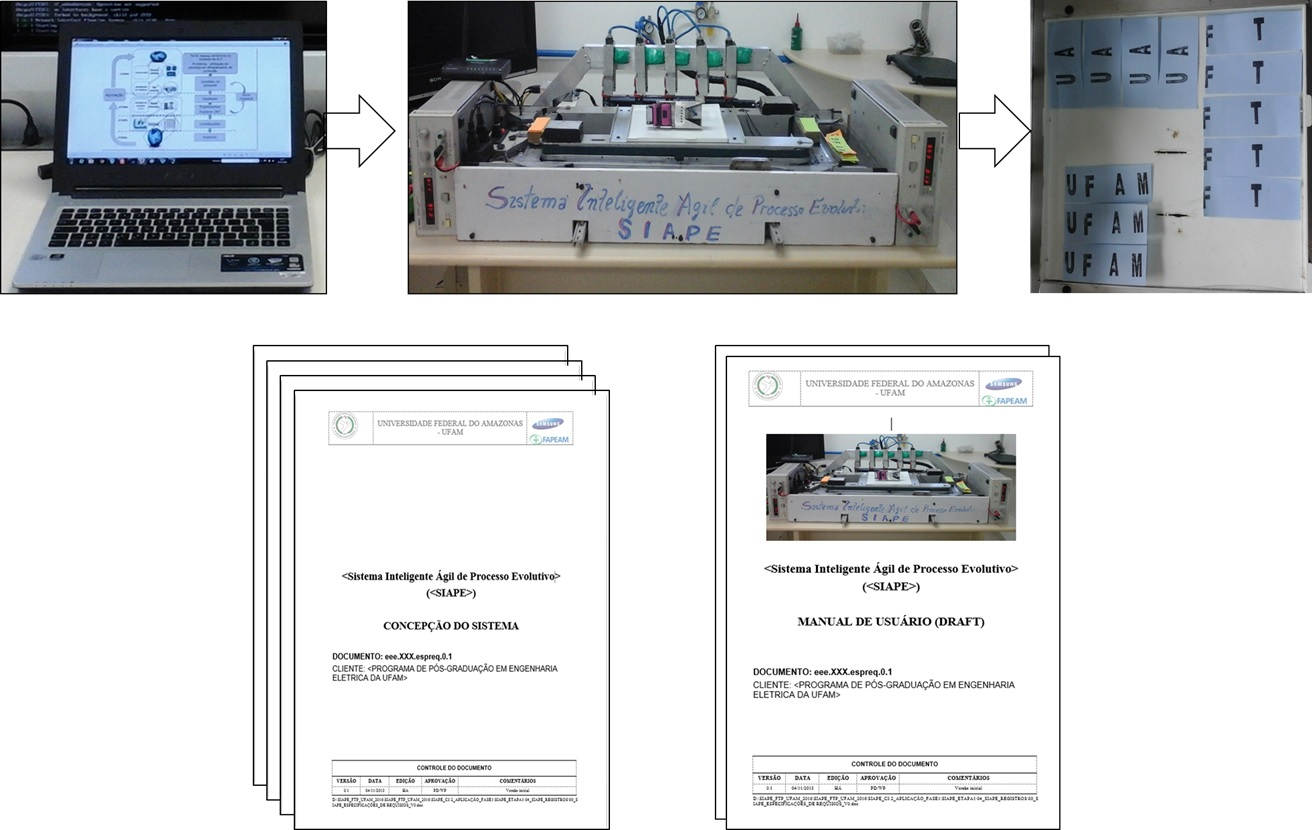
\includegraphics[width=16cm, height=9cm]{F100_SIAPE_COMISSIONAMENTO.jpg} 
	\caption{Etapa de Comissionamento}
	\label{F100}
\end{figure}

A Etapa de Comissionamento é fundamental para a realização de testes finais onde possa mapear as entradas e saídas de dados para incluí-las nos manuais técnicos  e de usuário. Esse mapeamento deve ser consolidado e incluído, se ainda não foi, nos documentos que serão entregues ao cliente. \par 
O fechamento do nono marco é evidenciado pela entrega dos documentos técnicos e de usuários concluídos aso responsáveis em realizar a Etapa de Entrega junto ao cliente e seus especialistas. É sempre uma boa prática acompanhar as verificações e participar, na prática, das operações de comissionamento. Isso dará mais segurança no trato com o cliente.

%=================================== ETAPA 10 ==================================

\clearpage
%+++++++++++++++++++++++++++++++++++++++++++++++++++++++
\subsection{ETAPA 10 - ENTREGA}

\begin{table}[htbp]
	\centering
	\caption{Tabela da etapa 10 - Entrega}
	%=================================================================================================
	\begin{tabular}{|l| p{13.5cm}| c| c| } \hline
		%================================================================================================
		\textbf{Item} 	    & \textbf{Descrição} 
		\\ \hline
		%================================================================================================
		\textbf{1.Objetivos}	   &  
		Realizar a entrega oficial do SIAPE, agora com o status de produto, ou seja, é o teste de aceitação do produto desenvolvido realizado pelo cliente sob a orientação da equipe de desenvolvimento. 
		\\ \hline
		%================================================================================================
		\textbf{2.Entradas}	  &		
      
		Produto SIAPE,  Manual de usuário, Manual técnico com especificações técnicas e Requisitos iniciais do cliente. 
		\\ \hline	
		%================================================================================================	
		\textbf{3.Processo}     &
		O produto SIAPE é submetido aos testes de aceitação do cliente.
		\\ \hline
		%================================================================================================
		\textbf{4.Saídas}		& 
		A saída do processo é o produto SIAPE aprovado pelo teste de aceitação do cliente.
		\\ \hline
		%================================================================================================		
		\textbf{5.Registros}   & 	
		Manual de usuário, Manual técnico e Requisitos iniciais do cliente.
		\\ \hline
		
		%================================================================================================
		\end{tabular}
	\label{T12}\par
	%	Fonte: Hiram Amaral
\end{table}


\begin{description}
	
\item[Descrição textual e visual da etapa]
O Produto SIAPE aprovado é submetido à Etapa de Entrega. Essa etapa se configura pela realização do teste de aceitação do cliente sob a orientação da equipe de desenvolvimento. No momento da realização dos testes, todos as observações e solicitações devem ser anotadas para que se verifique a possibilidade de inclusão, se a observação estiver dentro do escopo do projeto, ou não, se estiver fora do escopo, neste último caso, uma nova negociação deve ser realizada.    

\end{description}

%+++++++++++++++++++++++++++++++++++++++++++++++++++++++

A Figura \ref{F101} ilustra a finalização do processo de desenvolvimento por meio da entrega do Produto SIAPE ao cliente. Neste momento, o estudo de caso utilizado na Fase de Finalização é realizado pelo cliente, e seus especialistas, sob a orientação da equipe de desenvolvimento. O manual de usuário é explicado e realizado em sua íntegra para que não hajam dúvidas de sua aplicabilidade ao produto desenvolvimento.  

\begin{figure}[h]
	\centering
	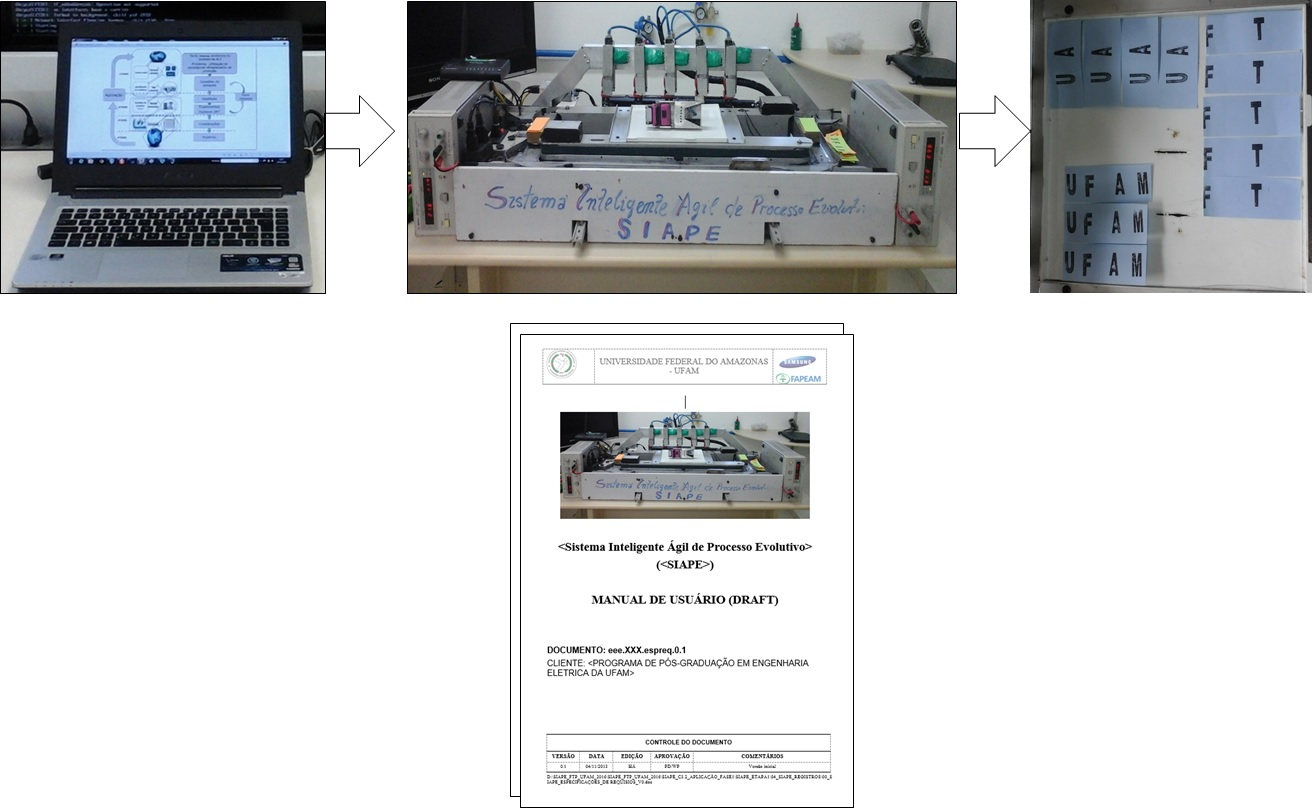
\includegraphics[width=16cm, height=10cm]{F101_SIAPE_ENTREGA.jpg} 
	\caption{Etapa de Entrega}
	\label{F101}
\end{figure}

É importante notar que, ao término da Etapa de Comissionamento, o sistema não é apenas um projeto de sistema realizado, mas atingiu o status de produto com seus manuais, especificações e requisitos atendidos e prontos para serem submetidos à validação do cliente. 

Esse produto realizado trata-se do sistema evolutivo, denominado de SIAPE, que foi desenvolvido durante as dez etapas de desenvolvimentos contidas no Método de Desenvolvimento de Sistemas Evolutivos (MeDSE), elaborado especificamente parar suprir a necessidade de desenvolvimento de sistemas que são baseados no paradigma evolutivo de produção (EPS), aderentes aos ambientes da \iQuatroZero~e preparado para a \textit{IoT}.



